\documentclass[12pt]{book}
\DeclareUnicodeCharacter{0300}{\`}
\DeclareUnicodeCharacter{0301}{\'}

\usepackage{url}
\usepackage[utf8]{inputenc} % This defines the font-encoding you prefer to use
\usepackage[pdftex]{graphicx}
\usepackage[margin=2cm,bindingoffset=1cm,centering,includeheadfoot]{geometry}

\usepackage[
    citestyle=numeric-comp,
    backend=biber,
    bibencoding=inputenc
    ]{biblatex}
\addbibresource{refs.bib}


\usepackage{setspace}
\linespread{1.5}
\setcounter{tocdepth}{2}
\usepackage[colorlinks=true, pdfstartview=FitV,
linkcolor=blue, citecolor=blue, urlcolor=blue]{hyperref}
\usepackage{cleveref}
\usepackage{xcolor}
\usepackage{xparse}

\setlength{\parindent}{0pt} % No indentation between paragraphs
\setlength{\parskip}{10pt} % Space between paragraphs

% Tables
\usepackage{ltxtable}
\usepackage{booktabs}
\usepackage{colortbl}


% Needed for code listings
\usepackage{listings}
\usepackage{color}

% Subfigure
\usepackage{subcaption}
\usepackage{floatpag} % to move floatpagenr to topright

% Fußnote
\usepackage[hang]{footmisc}
\setlength{\footnotemargin}{-0.8em}

\usepackage{csquotes}
\usepackage{afterpage} % needed for empty page after front

\usepackage[all]{nowidow} % prevents overhanging paragraphs
\usepackage{acronym} % allow acronyms

% The "num", "si", and "SI" commands for typesetting numbers, units, and numbers-with-units
%\usepackage[range-phrase=--,per-mode=symbol-or-fraction,binary-units=true,range-units=single,list-units=single,detect-all]{siunitx}
\usepackage[per-mode=symbol-or-fraction]{siunitx}
\usepackage{silence}\WarningsOff[latexfont]
\AtBeginDocument{
    \DeclareSIUnit\decibel{dB}
}


%%===================================
% Custom definitions
    
% Signal color
\definecolor{signalColor}{RGB}{164, 63, 114}
\newcommand\signal[1]{\textbf{\textcolor{signalColor}{#1}}}
    
% List with less space between items
\newenvironment{cList}{
\begin{itemize}
  \setlength{\itemsep}{0pt}
  \setlength{\parskip}{0pt}
  \setlength{\parsep}{0pt}
}{\end{itemize}}

% Enumeration with less space between items
\newenvironment{cEnum}{
\begin{enumerate}
  \setlength{\itemsep}{0pt}
  \setlength{\parskip}{0pt}
  \setlength{\parsep}{0pt}
}{\end{enumerate}}

% Space LoL
\let\Chapter\chapter
\def\chapter{\addtocontents{lol}{\protect\addvspace{10pt}}\Chapter}

% Rename listings and toc
\renewcommand{\contentsname}{Table of Contents}
\renewcommand{\lstlistlistingname}{List of Listings}

\NewDocumentCommand{\codeword}{v}{%
\texttt{\textcolor{orange}{#1}}%
}

\begin{document}

%%========================================
% Frontmatter

%!TEX root = ../thesis.tex

%This is the front page
%%=========================================
\thispagestyle{empty}
\begin{center}
    \huge{Revealing Challenges and Opportunities in Cycling Safety Through Crowdsourcing}\\[2pc]
    
    \large{vorgelegt von}\\
    \large{M.Sc.}\\
    \large{Ahmet-Serdar Karakaya}\\
    \large{ORCID: 0000-0002-2040-2782}\\[2pc]


    an der Fakultät IV – Elektrotechnik und Informatik\\
    der Technischen Universität Berlin\\
    zur Erlangung des akademischen Grades\\
    Doktor der Ingenieurswissenschaften\\
    - Dr. Ing. -
\end{center}

\begin{center}
eingereichte Dissertation
\end{center}

Promotionsausschuss:\\
Vorsitzender: Prof. Dr. Ziawasch Abedjan\\
Gutachter: Prof. Dr. David Bermbach\\
Gutachter: Prof. Dr. Heather Kaths\\
Gutachter: Prof. Dr. Odej Kao\\
\\
\begin{center}
April 2024
\end{center}

\afterpage{\null\thispagestyle{empty}\newpage}
 % This is the titlepage
\setcounter{page}{0}
\pagenumbering{Roman}
%!TEX root = ../thesis.tex

%This is the Preface
%%=========================================
\cleardoublepage
\section*{Sworn Affidavit}
\addcontentsline{toc}{section}{Declaration}

\begin{flushleft}
    I hereby declare that the thesis submitted is my own, unaided work, completed without any unpermitted external help. Only the sources and resources listed were used.\\
    \vspace{0.5cm}
    The independent and unaided completion of the thesis is affirmed by affidavit:\\
    \vspace{1.0cm}
    Berlin, April 9th, 2024
    \\
    \vspace{3.5cm}
    Ahmet-Serdar Karakaya
\end{flushleft}
 
%!TEX root = ../thesis.tex

%This is the Summary
%%=========================================
\cleardoublepage
\addcontentsline{toc}{section}{Abstract}
\section*{Abstract}
An increased modal share of bicycle traffic is a key mechanism to reduce emissions and solve traffic-related problems.
However, a lack of comfort and (perceived) safety keeps people from using their bicycles more frequently.
To improve comfort and safety in bicycle traffic, city planners need (a), an overview of accidents, near miss incidents, and bike routes, (b), an overview of the cycling infrastructure's maintenance state, and (c), a way to study the effect of potential changes in the cycling infrastructure before implementing them in the real life.
However, these needs, which are also of interest to cyclists and policy makers, are currently not being met satisfactorily.

In this thesis, we present three main contributions to solve these problems.
First, we show SimRa, a crowdsourcing-based citizen science project to record cycling trips and near miss incidents.
As part of this contribution, we also present CycleSense, an approach based on Deep Learning to automatically detect near miss incidents from recorded cycling trip data.
Knowing the hazardous bicycle traffic hotspots, policy makers and city planners can approve and implement safety improvements for cyclists.
Cyclists, on the other hand, can use this information to circumvent these spots.
Second, we describe an approach for deriving the road surface quality from cycling trip data.
Our approach uses data produced by the inertial measurement unit of the smartphone to calculate the smoothness of the road surface from the vibrations caused by traversing on the road with a bicycle. 
We then show how our approach can easily be integrated into a cycling trip recording app with SimRa as a case study.
This contribution also contains a visualization of the cycling infrastructure's smoothness and helps policy makers, city planners and cyclists in the same way as our first contribution.

Third, we improve the cyclist simulation model of the urban traffic simulation software SUMO.
For this, we first show that the default cyclist model of SUMO is not realistic by comparing it to cyclist behavior in the SimRa dataset.
We then split the cycling trips in the SimRa dataset into three parts for slow, medium, and fast cyclists and implement our findings as a plugin that can be added to SUMO for a more realistic cyclist simulation.
This new cyclist simulation can provide a strong tool for city planners to better to study effects of potential changes in the traffic infrastructure. 

\afterpage{\null\thispagestyle{empty}\newpage}
\addcontentsline{toc}{section}{Kurzdarstellung}
\section*{Kurzdarstellung}
Eine Erhöhung des Fahrradverkehrs trägt zur Verringerung der Treibhausgasemissionen und zur Lösung verkehrsbedingter Probleme bei.
Mangelnder Komfort und (gefühlte) Unsicherheit halten die Menschen jedoch davon ab, öfter Fahrrad zu fahren.
Um den Komfort und die Sicherheit im Radverkehr zu erhöhen, benötigen Stadtplanende (a) einen Überblick über Unfälle und Gefahrensituationen, (b) einen Überblick über den Wartungszustand der Radverkehrsinfrastruktur und (c) eine Möglichkeit, die geplanten Änderungen an der Radverkehrsinfrastruktur zu testen, bevor sie umgesetzt werden.
In dieser Arbeit präsentieren wir drei Beiträge zur Lösung dieser Probleme.

Zunächst stellen wir SimRa vor, ein Crowdsourcing-basiertes Citizen-Science-Projekt zur Erfassung von Gefahrensituationen im Radverkehr.
Im Rahmen dieses Beitrags stellen wir auch CycleSense vor, einen auf Deep-Learning basierenden Ansatz zur automatischen Erkennung von Gefahrensituationen aus aufgezeichneten Radfahrdaten.
Stadtplanende und politische Entscheidungstragende können die mit SimRa aufgedeckten gefährlichen Stellen im Radverkehr mit Baumaßnahmen verbessern.
Radfahrende können diese Informationen nutzen, um diese Stellen zu umfahren.

Im zweiten Beitrag beschreiben wir, wie wir die Straßenoberflächenqualität aus Fahrradfahrtdaten ermitteln.
Dazu verwenden wir Daten, die von den Bewegungssensoren des Smartphones erzeugt werden, um Unebenheiten der Straßenoberfläche anhand der Fahrtvibrationen zu berechnen.
Wir zeigen am Beispiel der SimRa-App, wie unser Ansatz in eine App zur Aufzeichnung von Fahrradrouten integriert werden kann.
Dieser Beitrag enthält auch eine Visualisierung der Ergebnisse und hilft sowohl Stadtplanenden als auch Radfahrenden.

Im dritten Beitrag verbessern wir das Radfahrersimulationsmodell der Verkehrssimulationssoftware SUMO.
Wir zeigen die Schwächen des Radfahrermodells von SUMO, indem wir es mit dem Verhalten von Radfahrenden im SimRa-Datensatz vergleichen.
Anschließend teilen wir die Radfahrten im SimRa-Datensatz in drei Teile für langsame, mittlere und schnelle Radfahrende auf und implementieren einen realistischeres Modell für SUMO.
Dies kann ein starkes Werkzeug für Stadtplanende sein, um ihre geplanten Änderungen an der Verkehrsinfrastruktur besser zu testen.
\afterpage{\null\thispagestyle{empty}\newpage}

\tableofcontents

\clearpage
\phantomsection
\addcontentsline{toc}{section}{\listfigurename}
\listoffigures

\clearpage
\phantomsection
\addcontentsline{toc}{section}{\listtablename}
\listoftables

\clearpage
\phantomsection
\addcontentsline{toc}{section}{\lstlistlistingname}
\lstlistoflistings

%%=========================================
% Mainmatter

%\cleardoublepage
\setcounter{page}{0}
\pagenumbering{arabic}
\part{Foundations}
\cleardoublepage
\chapter{Introduction}
\label{cha:introduction}
The global climate crisis is and will be one of mankind's most vital challenges in the first half of the 21st century and the effects thereof are already observable.
The frequency of extreme weather conditions and natural disasters such as long periods of precipitation leading to floods, or a lack of precipitation leading to droughts as well as heavy winds leading to storms is rising.
Such disasters have short and long term effects on the agricultural production of the affected areas leading to famine, conflicts and mass migration.
To prevent further aggravation of the effects, and stop or at least slow down the global warming, it is important to understand the root cause, so possible solutions can be derived and implemented. 
According to the \ac{ipcc}, the surface temperature of the globe has risen by 1.1°C during the period 2011-2020 when compared to the period of 1850-1900~\cite{lee2023climate}.
There is a consensus that this increase of the surface temperature is caused by anthropogenic emissions stemming from human activities such as deforestation and the burning of fossil fuels and thus releasing $CO_{2}$ and $NO_{x}$ to the atmosphere~\cite{archer2010climate}.
If the current trend of green house gas emissions continues, the Paris Agreement's~\cite{un2015paris} goal to keep the increase of the surface temperature of the globe under 2°C will not be met~\cite{noah2023data}.
That means that to stop or at least to slow down the global warming, a decrease of greenhouse gas emissions is needed as much and as fast as possible.
Reports published by the European Environment Agency of the European Union and the \ac{ipcc} of the United Nations indicate that transportation is one of the categories with substantial CO2 emissions~\cite{lee2023climate2}.
Cars cause over 70\% of the green house gas emissions, indicating that there is a big potential for savings.
More and more societies worldwide are aware of this problem and search for solutions to adapt to the new changes that comes with the climate change and try to decrease the impact of the global climate crisis.
This is why cities worldwide try to increase the modal share of bicycle traffic and by doing so, decrease the usage of motorized private transport.
The heavy usage of motorized private transport in urban areas also cause other problems.

First, there are the motor vehicle traffic crashes with an annual death toll of over 1.3 million and an annual injury toll of over 78.2 million.~\cite{bhalla2014transport}.
Additionally, these crashes can cause long-lasting psychological traumas for everyone involved, such as witnesses or police officers, health workers and firefighters that have to document the crash, help injured people and rescue people who are stuck in the car wreck.

Second, there are health issues that are indirectly caused by motorized private transport.
Transportation is one of the main causes for air pollution in urban areas in Europe~\cite{european2019european} and it is estimated, that around 8 million people die due to health issues that are connected to air pollution every year~\cite{forouzanfar2016global}. 
Motorized private transport causes air pollution in various ways.
Cars with an internal combustion engine produce (green house) gases such as CO2 or NOx as a byproduct from burning fossil fuels and particulate matter from the friction of the brakes and other car parts, as well as the friction between the tires and the street.

Third, noise pollution, to which car traffic undoubtedly also contributes significantly, also causes serious health issues~\cite{khreis2016health}.
Sleep and stress disorders, adverse reproductive outcomes are just some of the problems related to traffic noise.

Other problems of motorized private transport in urban areas and car-centric city planning are urban sprawl, which leads to less walkable cities~\cite{patacchini2009urban} and thus a more sedentary lifestyle, which in turn causes health issues stemming from a lack of physical activities, soil sealing, which damages biodiversity and the ecosystem~\cite{tobias2018soil} and many more ~\cite{bozovic2021non,pritchard2022maas,mayers2020whose}.  


\section{Problem Statement}
\label{sec:problem}
Since cities were developed with the motorized private transport as the main transportation mode in mind, the traffic infrastructure highly favors the usage of cars.
Because of that, cyclists often have a hard time commuting, since they have to cycle on roads that were made for cars, which often puts them into dangerous and stressful situations.
Although crash statistics do not convey an increased danger for cyclists (CITATION NEEDED), studies have shown, that the perceived safety of commuting with a bicycle is very low (CITATION NEEDED) and one of the main reasons why people prefer other transportation modes to cycling (CITATION NEEDED).
This poses a challenge to people who want to cycle, city planners and politicians alike.
People who want to cycle have to overcome their (perceived) lack of safety and comfort while commuting by bicycle to not feel forced to travel by car. 
It is up to city planners to improve the traffic infrastructure for cyclists, but it is not easy to pinpoint the most problematic areas, that need to be prioritized for them to be fixed, which is needed because of the limited resources available to the city planning department.
Besides, city planners are bound by city planning codes and rules, which oftentimes also reflect the car-centric approach.
This passes the responsibility to the politicians, who need to change the city planning codes and rules and also increase the funds for bicycle infrastructure.
For this, however, they need more than anecdotal evidence, that the perceived safety in bicycle traffic is low, so that they can change the legislation and increase funding in favor of bicycle infrastructure.

To enable city planners and politicians to do evidence-based decision-making, they need a) to be aware of the problems in bicycle traffic and b) to know where and how to improve the bicycle infrastructure.
Cyclists need good bicycle infrastructure that increase both safety and comfort of cycling, so that more and more people choose the bicycle over other modes of transport.
If the existing bicycle infrastructure is not good enough, they need to know which street sections are dangerous so that they can avoid them or be extra vigilant, when they have to pass through them.
Additionally, it would motivate cyclists to know that the problem is worked on and to keep the demand for a good bicycle infrastructure high. 

\section{Contributions of this Thesis}
\label{sec:contributions}

\section{Structure of this Thesis}
\label{sec:structure}

This thesis consists of four parts. Part I: Foundations begins with this chapter and proceeds with background information on the topics of  and an overview of the related work that are needed for a better understanding of the rest of this thesis. 
\cleardoublepage
\chapter{Background and Related Work}
\label{cha:background}
In this chapter, we go through fundamental topics that are needed to better understand the remainder of this work.

\section{Crowdsensing and Citizen Science}
\label{sec:crowdsensing_background}
Other edge-assisted data analysis work includes Mei et al.~\cite{mei2017ultraviolet}, who measure UV radiation based on smartphone cameras and crowdsensing,
Cao et al.~\cite{cao2015fast} who use motion sensors to detect strokes in patients falling to the ground, and
Pham et al.~\cite{pham2015a} implement a smart parking system by equipping parking spots with RFID chips to track their occupancy state.
There are also multiple publications on placing different components of an edge-to-cloud data processing pipeline in various use cases, e.g.,~\cite{lujic2021increasing,pfandzelter2021zero,hattab2019optimized}.

\section{Bicycle Traffic Safety}
\label{sec:bicycle_traffic_safety_related_work}
Other edge-assisted data analysis work includes Mei et al.~\cite{mei2017ultraviolet}, who measure UV radiation based on smartphone cameras and crowdsensing,
Cao et al.~\cite{cao2015fast} who use motion sensors to detect strokes in patients falling to the ground, and
Pham et al.~\cite{pham2015a} implement a smart parking system by equipping parking spots with RFID chips to track their occupancy state.
There are also multiple publications on placing different components of an edge-to-cloud data processing pipeline in various use cases, e.g.,~\cite{lujic2021increasing,pfandzelter2021zero,hattab2019optimized}.

\section{Near Miss Incidents}
\label{sec:near_miss_incidents_related_work}

\part{Improving Safety in Bicycle Traffic}
\chapter{Contributions}
\label{cha:contributions}


\chapter{Gathering Bicycle Ride Data and Detecting Near Miss Incidents in Bicycle Traffic}
\label{cha:cyclesense}
In recent years, more and more cities worldwide aim to reduce the modal share of car traffic in favor of bicycle traffic to reduce NO\textsubscript{x}, CO\textsubscript{2}, and particulate matter emissions, to reduce traffic jams, and to free up space that is urgently needed for other purposes ranging from vegetation that provides natural cooling in a heating world to new flats for a growing population.

A key mechanism to support this is to make bicycle traffic more attractive.
In practice, however, what keeps people from using their bikes more frequently is a lack of safety or perceived safety in cities with a car-centric traffic infrastructure~\cite{aldred2018predictors}.
Hence, city planners urgently require an overview of safety and perceived safety in their city.

Aside from actual accidents, an often overlooked aspect of cycling safety are near miss incidents\footnote{In the remainder of this paper, we will also refer to them as ``incidents''.} such as close passes or near dooring~\cite{aldred2018predictors, karakaya2020simra}.
Information on these have previously not been available or have not been easily accessible as they are distributed over private video recordings, social media posts, public CCTV footage, and other sources.
In 2019, we therefore launched the SimRa\footnote{SimRa is a German acronym for safety in bicycle traffic.} project in which cyclists record their rides and annotate them with incident information via a smartphone app~\cite{karakaya2020simra}.

While our previous approach~\cite{karakaya2020simra} already used a rudimentary heuristic for automatically detecting incidents based on acceleration sensors, it is inherently limited resulting in significant manual annotation efforts which makes it unattractive for some groups of cyclists -- in particular, elderly cyclists who have problems using smartphone apps and cyclists with significant daily mileage for whom the labeling approach is too much effort.
To increase participation, it is hence crucial to decrease manual efforts through an improved pre-detection of incidents.

As a first step towards this goal, we supervised a master's thesis which developed a neural network-based method for incident detection using the public SimRa data set\footnote{https://github.com/simra-project/dataset}~\cite{sanchez2020detecting} which, however, does not show the desired detection quality despite being an improvement over our original heuristic.
Both detection methods are currently used in the live version of the app, hence, we will later use them as baseline in our evaluation.
Besides that, there are alternative approaches for quantifying the perceived safety of bicycle traffic, e.g.,~\cite{blanc2016modeling, blanc2017safety, wu2018predicting}, but to the best of our knowledge no other methods are based on mobile motion sensory data.

Since its start in 2019, the SimRa data set has grown to more than 65,000 rides with almost 30,000 reported incidents.
These amounts of data now enable the application of much more sophisticated methods, namely \ac{ml} and/or \ac{dl}, for automatic incident detection.
Therefore, we here propose CycleSense -- a \ac{dl} model trained on smartphone sensory data from the SimRa data set to detect incidents in the SimRa app.
We hope, that it will lead to more reported incidents due to an easier reporting, and make the following contributions:

\begin{itemize}
	\item We propose an approach that combines signal processing and \ac{ml} techniques to detect incidents based on motion sensor data of cyclists with an \ac{auc} \ac{roc} of 0.906 (Section~\ref{sec:detecting}).
	\item We evaluate our approach using the SimRa data set and compare it to two baselines as well as common \acl{dl} models used in the context of \acl{tsc} (Section~\ref{sec:eval}).
	\item We discuss to which degree our approach can automate incident detection and which additional sensors are needed for full automation (Section~\ref{sec:disc}).
\end{itemize}

\section{Deep Learning}
\label{sec:deep_learning_background}
One of the most common tasks for \ac{tsc} are Natural Language Processing, speech recognition, and audio recognition in general.
Another field that deals with this problem is \acf{har} which is concerned with identifying the specific activity of a human based on sensory time series data.
Time windows of a few seconds are classified into activity categories (e.g., walking, sitting, running, lying).
While various feature extraction and pattern recognition methods have been successfully applied in the past in this context~\cite{bulling2014tutorial}, those approaches have constraints such as hand-crafted feature extraction, being able to only learn shallow features~\cite{yang2015deep}, or the requirement for large amounts of well-labeled data for model training~\cite{wang2019deep}.
\acl{dl} techniques and more specifically \acp{cnn} have recently proven to overcome these issues and deliver convincing results in the context of \ac{har}~\cite{wang2019deep,ronao2015deep}.
Also, implementations of \acp{rnn} such as \ac{lstm}~\cite{tao2016multicolumn,yao2017deepsense} have proven to be successful.
Yao et al.\ \cite{yao2017deepsense} use a combination of \acp{rnn} and \acp{cnn} on top of a \ac{sf} approach after preprocessing their input data using a \ac{dft}.


\section{SimRa - A Platform for Gathering Bicycle Rides and Near Miss Incidents in Bicycle Traffic}
\label{sec:simra}

\subsection{Goal of the SimRa platform}
\label{subsec:simra}
In this section, we give a general overview of the SimRa platform which comprises all things related to the collection, storage, and analysis of crowdsourced cycling data which we will focus on in the following sections.

For data acquisition we rely on an app installed on the smartphones of participating cyclists.
This app collects data and detects incidents during rides, lets users add comments or labels, and anonymizes the data before uploading it to our servers (see section~\ref{sec:data_acquisition}).
The anonymized data comprises information on cyclist routes, incidents, user demographics, as well as some aggregated ride statistics (see section~\ref{sec:data}).
Finally, we continuously process and analyze collected data to gain insights into dangerous street segments and intersections.
For this, we have developed one approach for interactive exploratory data analysis based on a web application and one for confirmatory data analysis~\cite{bermbach2017cloud} which automatically derives a ``dangerousness'' score per street segment and intersection (see section~\ref{sec:analysis}).

\subsection{Data Acquisition}
\label{subsec:data_acquisition}
Our approach relies on crowdsourcing to collect necessary data; in fact, SimRa is a citizen science project.
For data acquisition, we could either rely on dedicated hardware or use commonly available hardware such as smartphones.
While dedicated hardware has certain benefits, e.g., higher measurement precision, such projects are inherently limited in scale:
\begin{figure}
    \center
    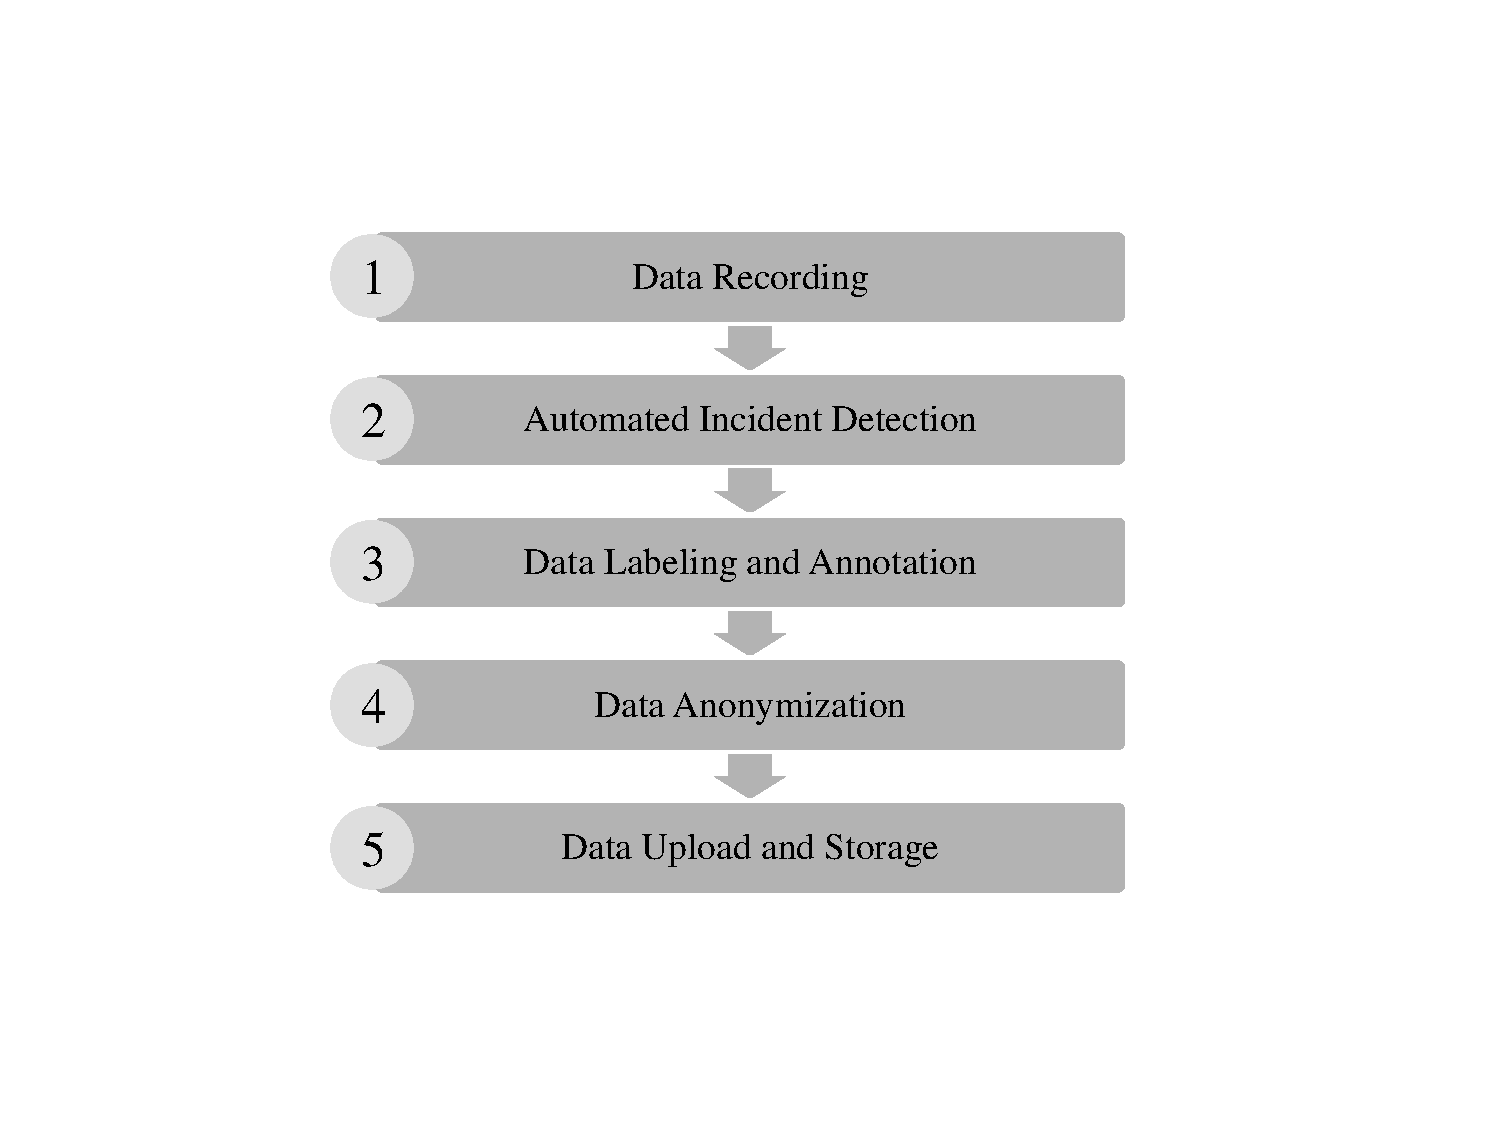
\includegraphics[width=0.5\columnwidth]{fig/data_acquisition_process.pdf}
    \caption{In the data acquisition process, collected data is manually annotated and anonymized before being uploaded to our backend servers.}
    \label{fig:data_acquisition_process}
\end{figure}
%An example of this is the Radmesser project~\cite{ndw_2019} which built custom sensors to track close pass incidents.
%While the data quality is indeed rather high, the project was limited to a total of 100 cyclists (only partly in parallel).
%As a result, the project could not achieve full coverage of Berlin streets.
%For example, one of the incident hotspots in terms of close passes that we were able to identify in SimRa did not even have a single ride in the Radmesser data.
We decided for project scalability and collect data with smartphones only.
Our goal is to collect data in a way that allows us (i) to identify incident hotspots as well as the kind of incidents and (ii) to identify the routes of cyclists (in which unnecessary detours are likely to identify severe incident hotspots).
%, and (iii) to collect additional data with the goal of improving automated incident detection.


Overall, our data acquisition process has five steps and follows the structure shown in figure~\ref{fig:data_acquisition_process} (we describe the steps in the following sections in detail).
This process runs continuously and in parallel as cyclists may create data for individual rides at any time.
During a ride, we first record sensor data using the built-in sensors of a cyclist's smartphone.
Upon completion of a ride, we analyze the raw data to automatically detect incidents.
Afterwards, the cyclist can enrich collected data with labels and annotations, use a number of anonymization measures, and upload the data to our backend servers.

\paragraph{Data Recording}
During a ride, we track three sensors at varying rates per minute.
First, we query the GPS sensor every three seconds; this returns the current location and a radius with an accuracy confidence value of 68\%.
Second, we query the smartphone's accelerometer at 50Hz.
%These values include the effects of gravity and are in $m/s^2$.
While such a high sampling rate allows us to detect sudden peaks, this also leads to an unnecessary large data set which typically needs to be uploaded via mobile networks.
Thus, we aggregate the data based on a moving average across 30 values of which we only consider every sixth value.
This reduces the amount of data while still retaining all peaks in sensor readings.
Third, we store the device orientation based on the smartphone's gyroscope sensor every three seconds.
%These values describe the rate of rotation around the X/Y/Z axis in rad/s and allow us to correctly interpret the direction of the acceleration values.
Each sensor measurement, together with a timestamp, is stored locally on the device.

We chose these rate settings based on initial experiments in which we identified the data collection rates and aggregation schemes as a sweet spot between system overload and information loss.



\paragraph{Automated Incident Detection - Naive Approach}
After a ride, as soon as the cyclist stops the recording, we analyze the recorded data to identify incidents.
The challenge, here, is to reliably detect incidents -- initially, without any training data.

For this reason, we developed a heuristic for incident detection that relies on the assumption that incidents will often materialize as sudden acceleration spikes.
Now, that we have over 10,000 labeled rides, we started to explore alternative detection methods ranging from machine learning to signals processing.
In our heuristic, we group the acceleration time series in three-second buckets to differentiate incidents and poor road conditions (e.g., potholes result in high vertical acceleration).
In each bucket, we identify the minimum and maximum value for every dimension and calculate the difference between those two.
In a second step, we categorize the six highest difference values across all buckets as likely incidents.
This allows us to separate high acceleration values based on poor road conditions (which usually have low difference values) from incident-related peaks.

In practice, this heuristic works well for cyclists with a ``relaxed'' cycling style.
For cyclists with a more ``rapid'' style of cycling, our heuristic usually identifies either accidents, severe bumps, or traffic lights but usually not incidents.
The heuristic is also inherently limited as it cannot detect close passes and similar incidents which do not materialize as acceleration spikes.

\paragraph{Data Labeling and Annotation}

Even though we plan to improve the automated detection of incidents, some incident types cannot be automatically detected based on the sensor data alone.
For example, while being tailgated might make the cyclist ride faster, this kind of observable activity can also be related to other, non-dangerous events.
Thus, we do not think that a fully automated detection, also based on our hardware limitations, is a realistic option for SimRa -- neither now nor in the future.
Instead, we ask the cyclist to edit the pre-detected set of incidents (i.e., add false negatives and ignore false positives) and to label and annotate the correct set of incidents (see also section~\ref{sec:data} which describes the resulting data in detail).

\paragraph{Data Anonymization}

One of our side goals in SimRa is to preserve the privacy of our users, which is mainly achieved through three mechanisms: \emph{Delayed recording} allows users to define a time and a distance threshold after which a recording will start, \emph{ride cropping} allows users to crop their ride manually to hide where they started or arrived, and \emph{per-record pseudonymization} stores demographic and ride data separately so that rides cannot be connected to individual users. Furthermore, each ride is pseudonymized separately.


%\begin{itemize}
    %\item Delayed recording: Users can define a time and a distance threshold after which a recording will start
    %\item Ride cropping: Users can crop their ride manually to hide where they started/arrived
	%\item Per-record pseudonymization: Demographic data and ride data of users is stored separately, so that rides cannot be connected to individual users. Furthermore, each ride is pseudonymized separately.
%\end{itemize}


\paragraph{Data Upload and Storage}
Finally, and only when explicitly triggered by the cyclist, the ride data is uploaded to our backend.
For authentication, we calculate an access key based on the current timestamp and a random salt which we update with new app versions.
This is necessary to avoid automated attacks on our backend as we do not have a notion of user accounts.
So far, this has sufficed as extracting the salt from the app binary requires enough manual effort to make this infeasible for automated attacks.
Note, that we store rides and user data per region so that we can analyze (geographic) regions separately (we describe our concept of regions in section~\ref{sec:data}).


\section{Detecting Near Miss Incidents with Deep Learning}
\label{sec:detecting_near_miss_incidents}
This section describes the process of automatically detecting incidents. 
Please note that the SimRa data are not optimized for automated processing and \ac{ml} but rather for aggregated statistics and review by humans.
Therefore, several preprocessing steps are needed (Section~\ref{subsec:preprocessing}).
We describe our \ac{ml} model in Section~\ref{subsec:architecture} and the training process in Section~\ref{subsec:training}.


\subsection{Preprocessing}
\label{subsec:preprocessing}
To overcome some limitations of the SimRa data set, we use data cleaning and preprocessing steps, in a sequential multi-stage manner,  some of which are specific to some model types that will be used afterwards to classify the incidents within rides.

Before the preprocessing phase, a typical ride can be expressed by a $n \times d$ sparse matrix $X^{(i)}$, where $d$ describes the number of sensor features and $n$ represents the number of timestamps in a given ride $i \in \{1,...,R\}$.

Note that we typically only use the accelerometer, gyroscope, and \ac{gps} sensor features.
Using the linear accelerometer features in addition did not lead to a significant improvement.
Furthermore, the linear accelerometer and the rotation vector features are only available in the newer Android rides.
The non-sensory features such as phone location and bike type have a non-logical strong correlation with incidents caused by issues in the data recording phase and are therefore not used.

\begin{figure}[t]
	\centering
	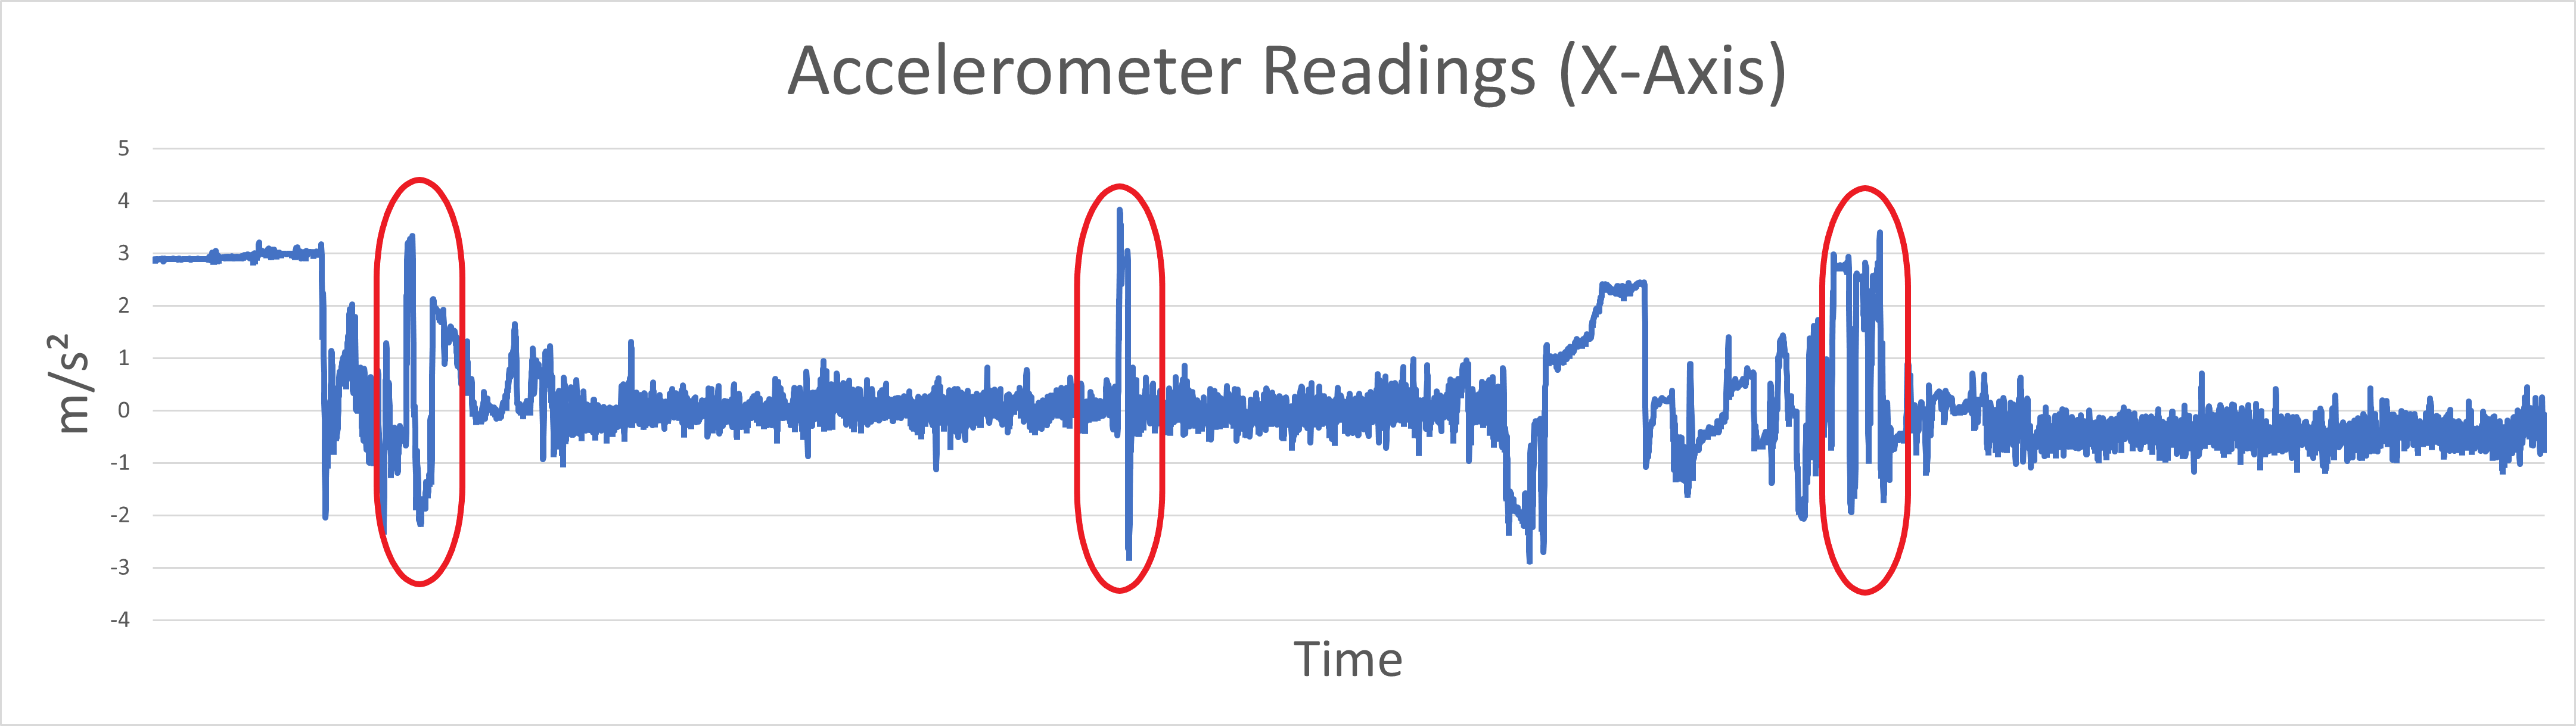
\includegraphics[width=0.5\textwidth]{fig/accelerometer-x-axis.png}
	\caption{The accelerometer readings of an example ride. The encircled spots could indicate an incident but also driving over a curb.}
	\label{fig:x-axis}
\end{figure}

The preprocessing pipeline starts off with a manual label cleaning procedure that aims to remove some of the wrongly labeled incidents.
Identifying them solely based on time series data is practically impossible for a human.
When visualizing the accelerometer sensor readings, incidents usually stand out as sudden spikes (see Figure~\ref{fig:x-axis}), but they also could be caused by driving over a curb or suddenly stopping due to a red light.
Therefore we focus on the incidents that feature an additional description that was provided by the users.
As it is very time-consuming, this is the only manual preprocessing step, and we apply it only to the newer Android data set.
Note that this procedure did not result in a fully cleaned data set.
Next, the timestamps within rides are sorted.
Afterwards, we sort out invalid rides, i.e., rides that contain adjacent timestamps that have been recorded with a gap of more than 6 seconds.
Furthermore, we remove outliers based on the statistical definition of outliers by Tukey et al.~\cite{tukey1977exploratory} that characterizes a data point as an outlier if it fulfills one of the equations $Outlier < q_{25} - k \cdot IQR$ or $Outlier > q_{75} + k \cdot IQR$ where the \ac{iqr} is equal to the difference between the upper and lower quartiles \cite{upton1996understanding, zwillinger1999crc}.
The $k$-values we are utilizing are 1.5 for \ac{gps} outliers regarding the accuracy feature and 3.0 for velocity outliers, as we have seen reasonable results for these values.

In a further step, speed is calculated from the distance between two \ac{gps} coordinates and their respective timestamp.
Moreover, the accelerometer and gyroscope sensor data are interpolated to create equidistance over the whole time series.
This is advisable, as unevenly spaced time series data tend to pose a problem to typical \ac{ml} solutions~\cite{weerakody2021review}.
Therefore, we up-sample to a frequency of 10 Hz via linear interpolation on uniformly generated timestamps with a 100 ms interval.
That means the up-sampling factor is usually above 2.
Although some argue that interpolation is a bad solution for unevenly spaced time series data in the context of \ac{tsc}~\cite{hayashi2005covariance, eckner2012framework}, initial experiments have shown that this improves model performance.
This preprocessing stage results in dense matrices $X^{(i)}$

For better convergence of the stochastic gradient descent optimizer used in the neural network, we normalize each feature individually by its maximum absolute value.
This is nearly always an advantageous preprocessing step as it improves model stability~\cite{bishop1995neural}.

Training the model on individually labeled timestamps did not appear to be a promising approach since incidents have a certain duration, which is typically longer than 100 ms, and it is highly unlikely that the user correctly specifies the label at the exact timestamp when the incident occurred.
For that reason, we split our ride data into 10-second buckets, following a non-overlapping sliding window approach~\cite{ortiz2011dynamic}.
These buckets are then labeled in the following manner: we define a bucket as an incident bucket if any timestamp inside that bucket was labeled as an incident.
Otherwise, we define it as a non-incident bucket.

Additionally, we apply a one-dimensional $f$-point \ac{dft} on each dimension of the accelerometer and the gyroscope sensor data contained in a bucket individually.
This results in a more advanced temporal feature extraction approach that exploits the spectral power changes as time evolves by converting the time series from the time domain to the frequency domain~\cite{chen2021deep}.
%An overview of the process is illustrated in Figure~\ref{fig:fft}

%\begin{figure}[t]
%	\centering
%	\includegraphics[width=\textwidth]{fig/fftDetailed.png}
%	\caption{The process of stacking raw sensor signals into buckets and applying \ac{dft}~\cite{chen2021deep}.}
%	\label{fig:fft}
%\end{figure}

To cope with the heavy label imbalance (e.g., $\approx$ 1 : 170 on rides that have recently been recorded on Android devices) that is present in the data, we use a \ac{gan} with a \ac{cnn} architecture to generate augmented data and thereby lower the imbalance gap by 10\% as this has shown to produce good results in our experiments.
The aforementioned $f$-point \ac{dft} is applied on these synthetic incident buckets as well.

\subsection{Model Architecture}
\label{subsec:model_architecture}
As our problem setting is similar to the \ac{har} task (see Section~\ref{sec:rw}), we build a customized \ac{ann} inspired by the DeepSense architecture proposed by Yao et al.~\cite{yao2017deepsense}.

In a first step, the network input is split based on the sensor that has produced it into accelerometer, gyroscope and \ac{gps} (i.e., velocity).
Simultaneously, the previously Fourier transformed accelerometer and gyroscope data are separated into their real and imaginary parts.

Then, \ac{sf} is applied, a method that considers each sensor individually in order to extract sensor-specific information~\cite{elmenreich2002sensor}. 
Furthermore, it also enables the application of different individual subnets that are varying in complexity for each sensor input.
Each subnet has three convolutional layers that use 64 kernels, kernel sizes between $(3,3,1)$ and $(3,3,3)$, and a stride size of $1$.
While in the first convolutional layer no padding is used, the second and third convolutional layers apply zero-padding which differs from the original DeepSense framework proposed by Yao et al.~\cite{yao2017deepsense}. 
Another difference is that we use 3D-convolution instead of the 2D- and 1D-convolution that were applied in the original model. 
3D-\acp{cnn} are more suitable for detecting spatiotemporal features compared to 2D-\acp{cnn}~\cite{tran2015learning}. 
The described convolutional layers are complemented by batch normalization layers to reduce internal covariate shifts~\cite{ioffe2015batch}, by \ac{relu} activation, and by Dropout layers for regularization.

Our addition of residual blocks is also a slight modification of the original framework. 
The reasoning behind that change is that, in some cases, deeper models might have difficulties in approximating identity mappings by multiple nonlinear layers~\cite{he2016deep}. 
Residual blocks have been applied with great success to overcome this issue~\cite{he2016deep}.

Next, the outputs of the different subnets are merged in a convolutional fusion network. 
Its architecture is similar to the individual subnets containing six convolutional layers, residual blocks, batch normalization, \ac{relu} activation, and Dropout. 
The full process is shown in Figure~\ref{fig:sfn}.

\begin{figure}[t]
\centering
    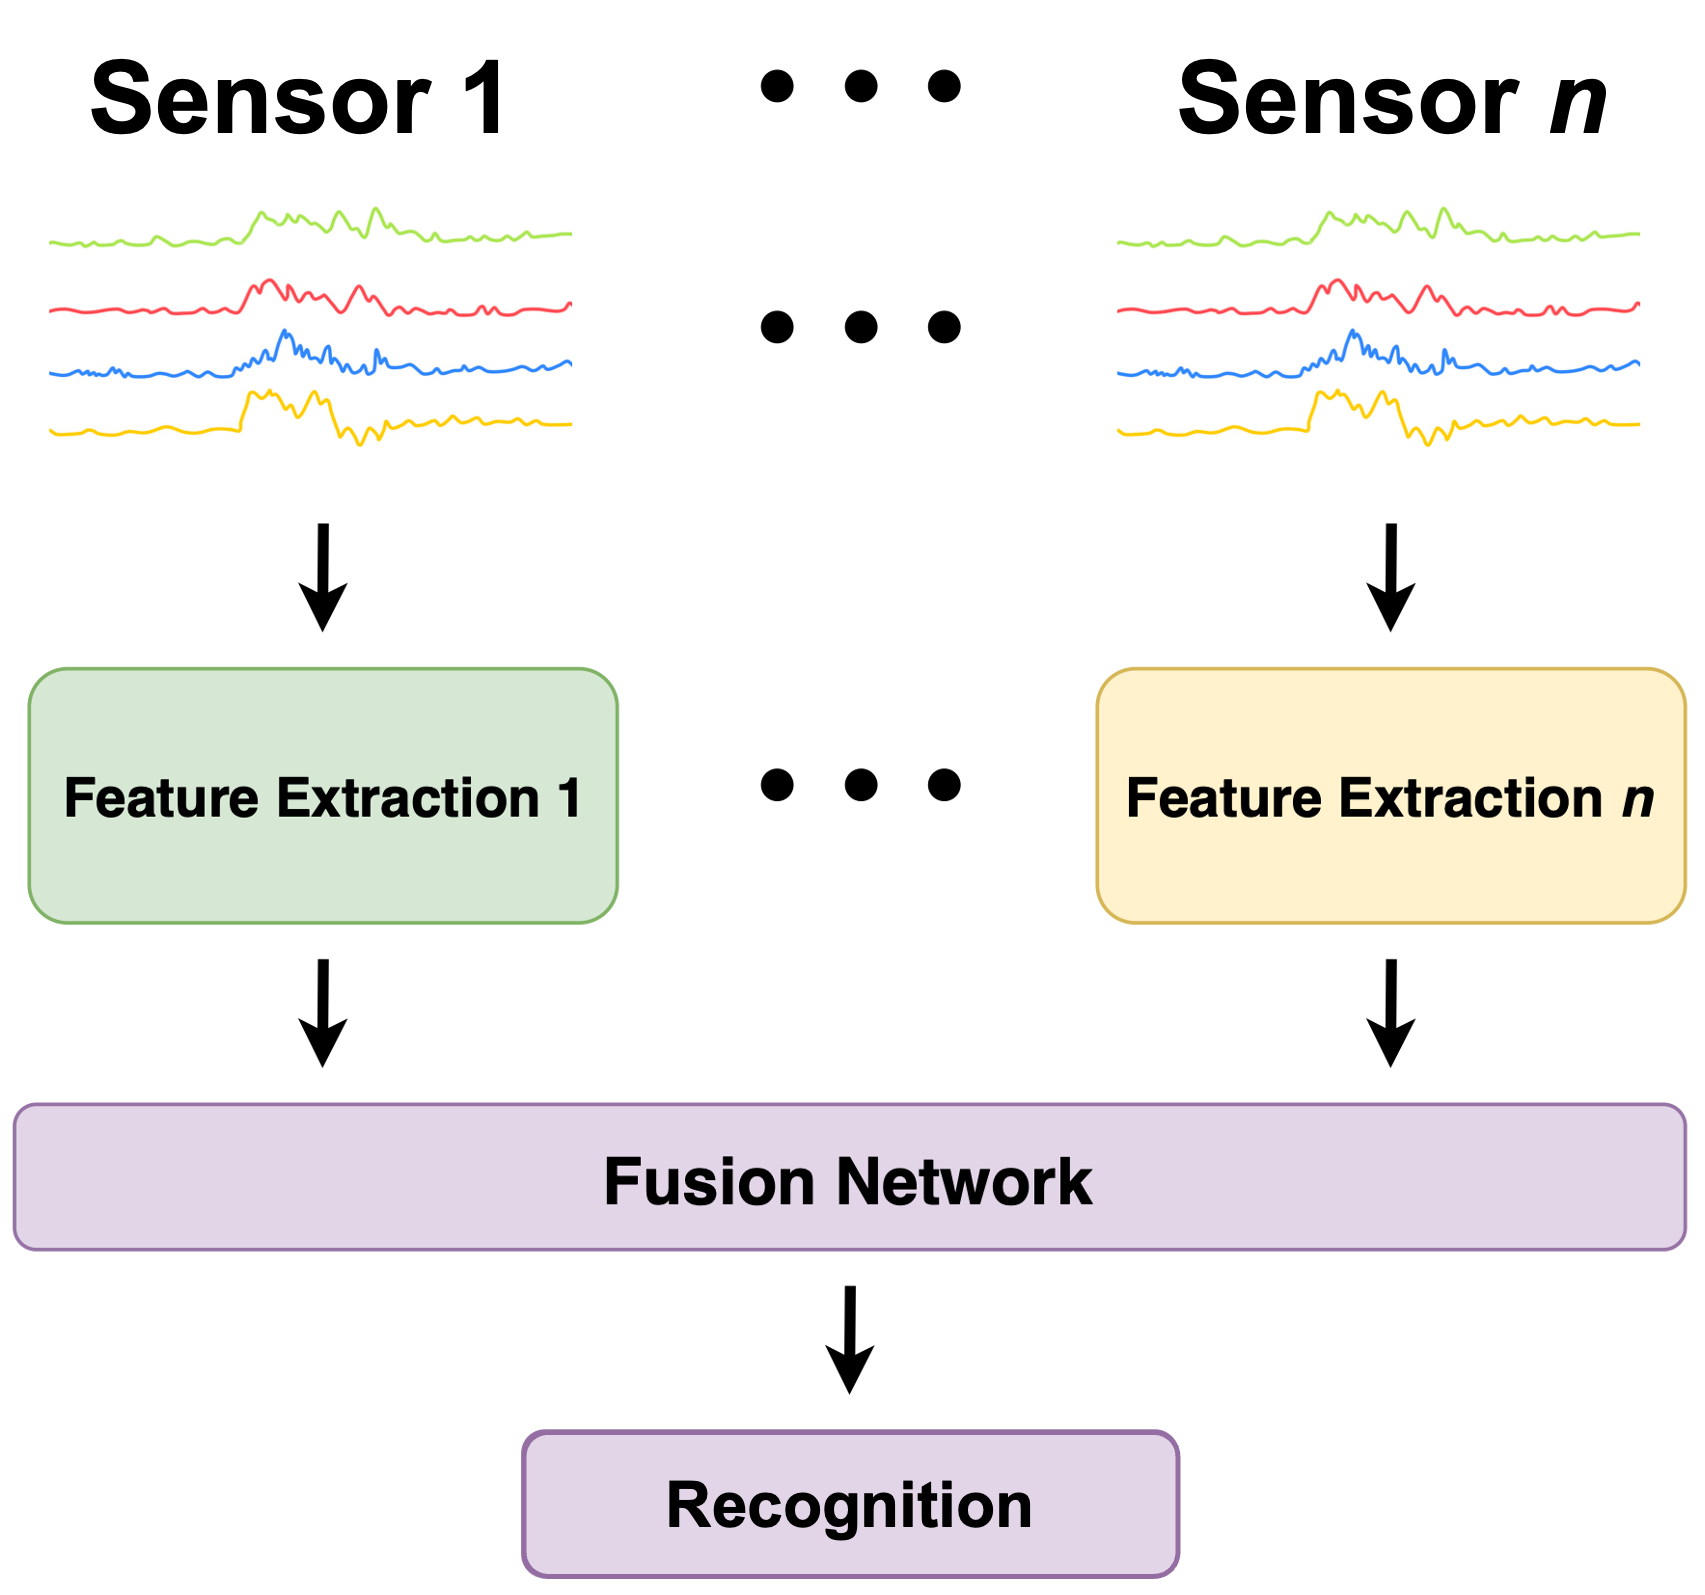
\includegraphics[width=0.4\columnwidth]{fig/sensor-and-fusion-networks.png}
    \caption{The model architecture in a nutshell: Using subnetworks for feature extraction of the different sensors (accelerometer, gyroscope, and \ac{gps}) and afterwards a fusion network to combine the features for final incident recognition~\cite{chen2021deep}.}
    \label{fig:sfn}
\end{figure}

The last big component of CycleSense is a \ac{rnn}.
\ac{rnn} architectures such as \ac{lstm}~\cite{hochreiter1997long} or \acp{gru}~\cite{chung2014empirical} are capable of holding information the network has seen before and using it to make predictions in the current state. 
In doing so, it is possible to identify patterns or relationships inside the timestamps of a bucket or between buckets. 
Similar to Yao et al.\ \cite{yao2017deepsense}, we also chose stacked \ac{gru} cells as they efficiently improve the model capacity~\cite{goodfellow2016deep}.

To determine the optimal set of parameters for training CycleSense, we have conducted a grid search on a variety of hyperparameters, some of which are shown in Figure~\ref{fig:hpo}.

In the following, we use \ac{gps}, accelerometer, and gyroscope data as model input if not indicated otherwise.  
Linear accelerometer data was only used in a few experiments as it is not available in our iOS and older Android data sets.
Our implementation of CycleSense is available on GitHub\footnote{https://github.com/simra-project/CycleSense}.

\begin{figure}[t]
	\centering
	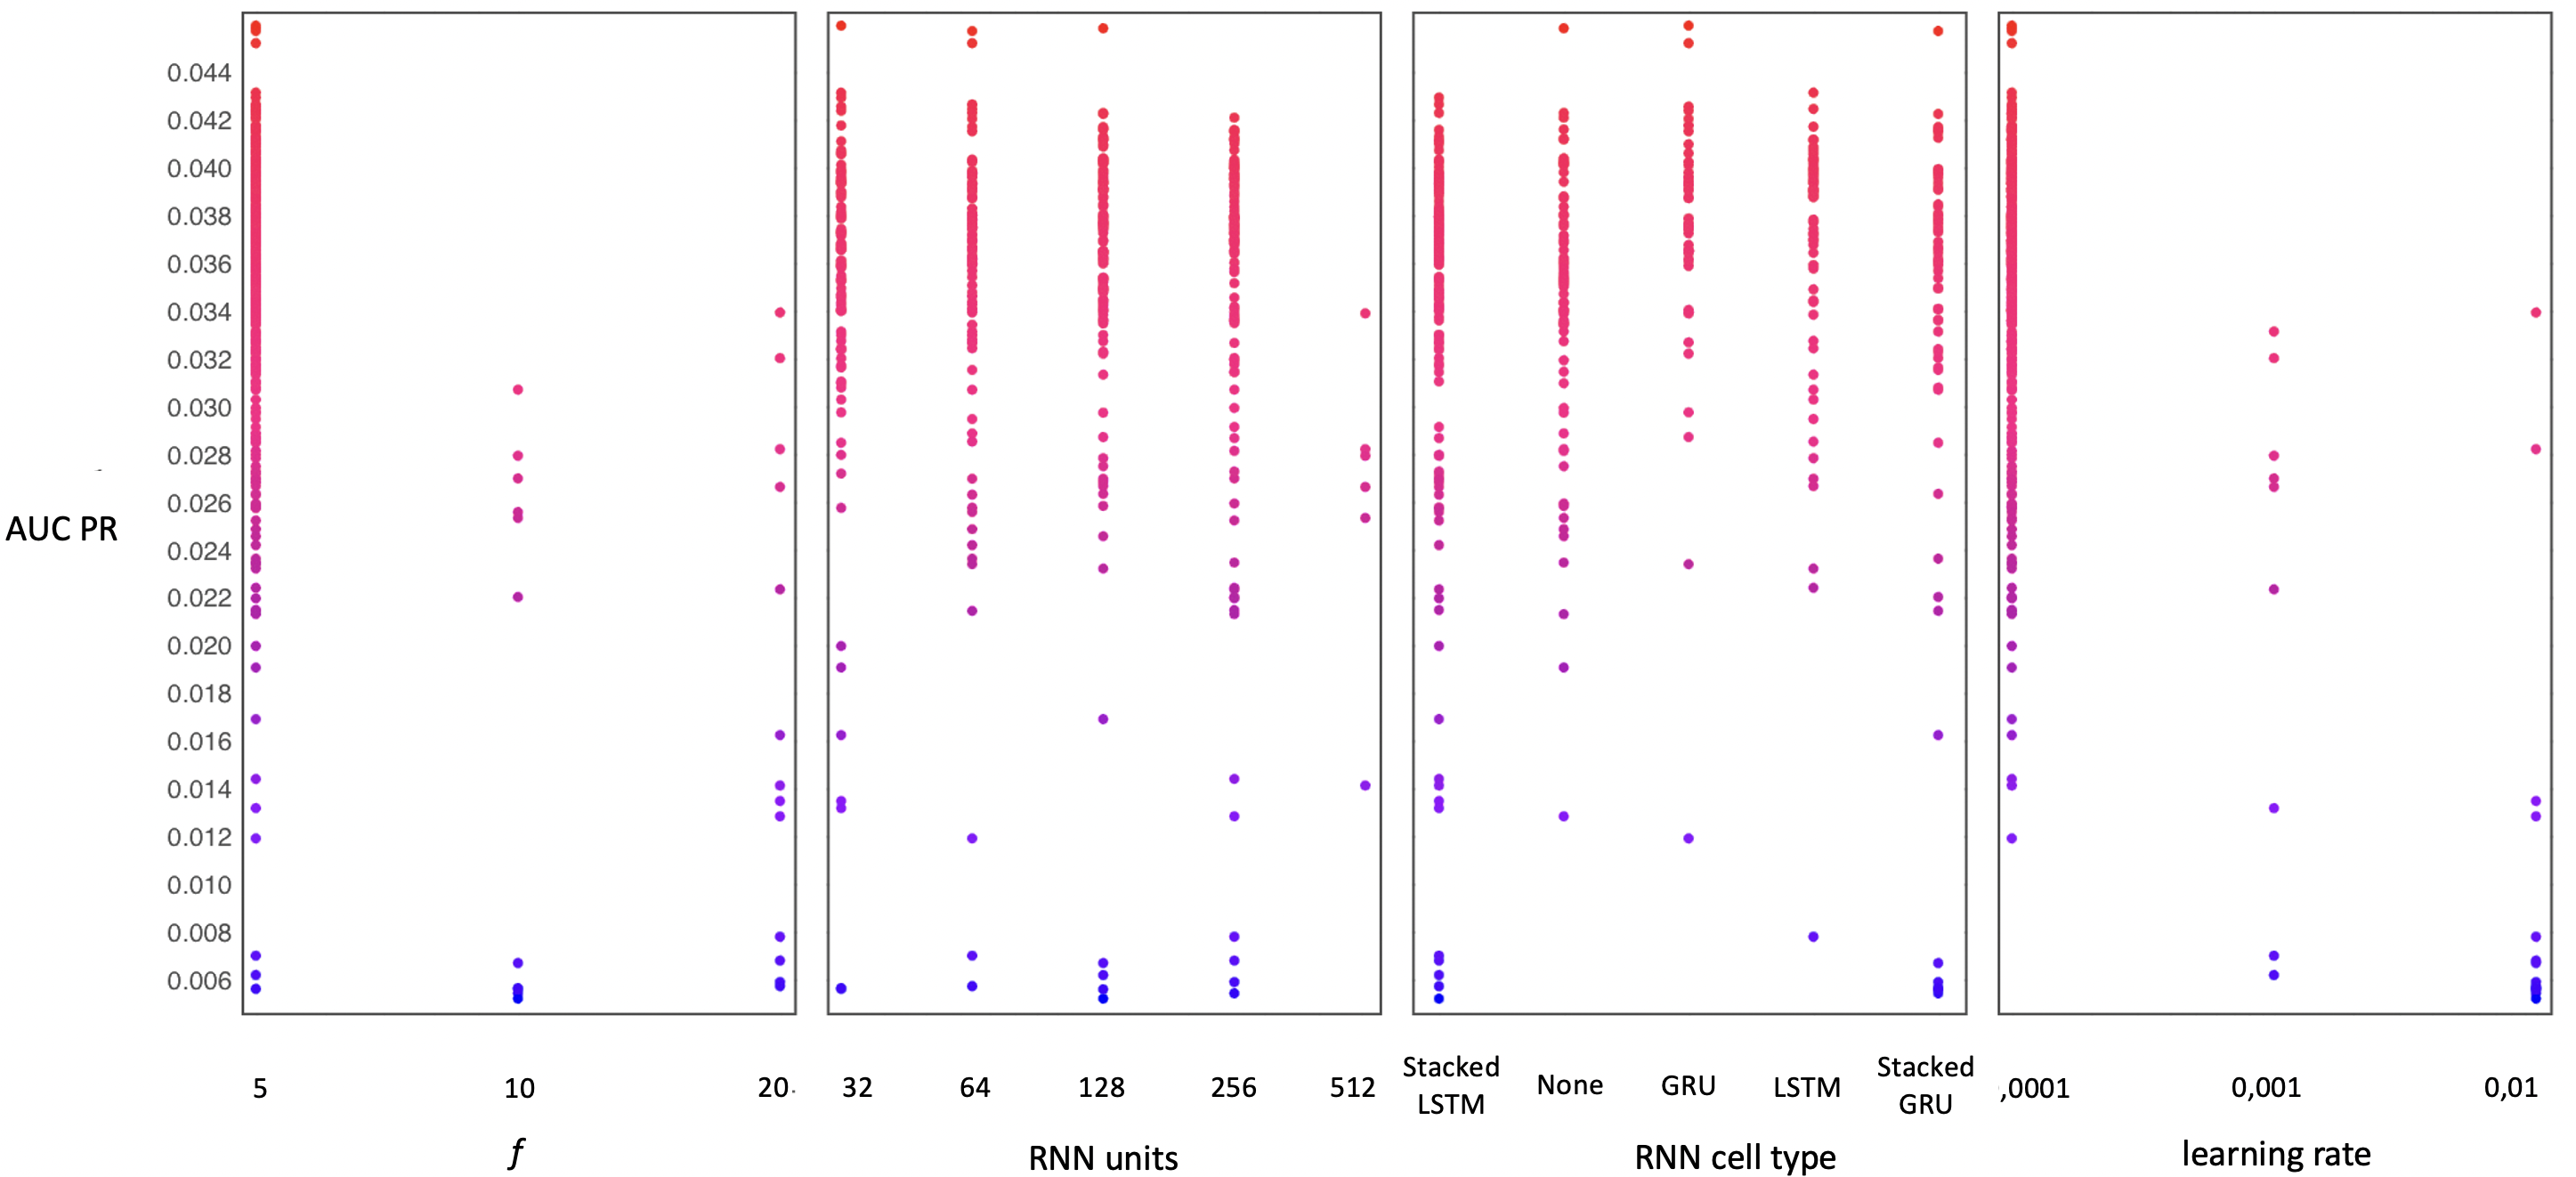
\includegraphics[width=\textwidth]{fig/hpo_results.png}
	\caption{Results of the hyperparameter optimization for the four variables $f$ (the window size), the number of \ac{rnn} units used, the \ac{rnn} cell type utilized, and the learning rate from left to right.}
	\label{fig:hpo}
\end{figure}

\subsection{Model Training}
\label{subsec:model_training}
For model training, the data set was split randomly into a training set (60\%), a validation set (20\%), and a test set (20\%).
Furthermore, the exact same splits are used for each model to improve comparability.
We trained the final model for 60 epochs on an NVIDIA K80 GPU.
We utilized a \ac{bce} loss function that was updated with Adam optimization, a \ac{sgd} method, a learning rate of 0.0001, and early stopping with a patience value of 10 epochs on the \ac{auc} \ac{roc} of the validation set.
It is important to note that we did not use the complete SimRa data set.
Instead, we used only a smaller subset of more recent rides recorded on Android devices since the heterogeneity of the data set across different versions and operating systems (see Section \ref{sec:disc}) did not allow us to train a model properly on the full data set.
In addition, due to limited access to hardware, we focused predominantly on data originating from the Berlin region if not stated otherwise.

As previously described, one notable challenge we were facing was the extreme label imbalance present in the data.
This is due to the fact that incident buckets are far rarer than non-incident buckets.
To cope with that, we trained our model by using a weighted loss function with the class weights of the train data set as weights.
For example, the class weights were 1 and 170 for the rides that have recently been recorded on Android devices.

While the DeepSense model was trained in a standard fashion, we use stacking during the training of CycleSense.
Stacking (or stacked generalization) is an ensemble learning method that combines the predictions of several different models in order to contribute equally to a collective prediction.

However, we are also not interested in equal contributions of the network since that could overvalue models with a poor performance.
We therefore changed the CycleSense model to an integrated stacking model by adopting the idea of stacked generalization~\cite{wolpert1992stacked}, where the fusion network acts as the meta-learner.
Also, we deviate from a pure stacking model.
This is the case, as the meta-learner does not get any classification output of the subnetworks as input aside from the latent features in the last layer of the subnetworks.
Thereby, the weights of the submodel layers that have been pretrained individually are loaded and frozen, so they are not updated during the training of the whole CycleSense model.
This learning procedure further improved our results as shown in Section~\ref{sec:disc}.

\section{Evaluation}
\label{sec:evaluation_cyclesense}
To evaluate CycleSense' training results, we have to put them into context. 
For this purpose, we compare them to the two detection methods currently used in the app as discussed in Section~\ref{sec:background}.
We give an overview of the changes we made to the baseline methods with the goal of a fair comparison in Section~\ref{subsec:baselines}.
We also describe the metrics that we use to compare our model to the baseline methods (Section~\ref{subsec:metrics}) before presenting the results of our evaluation (Section~\ref{subsec:eval-results}).


\subsection{Baselines}
\label{subsec:baselines}
The first baseline is our original heuristic~\cite{karakaya2020simra} which is based on the underlying assumption that incidents will often result in sudden acceleration spikes, e.g., when braking or swerving to avoid obstacles.
We made some small changes to this heuristic to enable its compatibility with the \ac{auc} \ac{roc} metric, thus, increasing the comparability with our approach.

As a second baseline, we retrained the \ac{fcn} model from the alternative approach~\cite{sanchez2020detecting}.
We used the original preprocessing pipeline (which differs significantly from the here presented one) but used the full data set as introduced in Section~\ref{sec:background}.
We skipped the under-sampling step, disregarded the phone location and the bike type feature for the reasons mentioned in Section~\ref{subsec:preprocessing}, and used a non-overlapping sliding window approach with 10 second windows for better comparability.

The third baseline is DeepSense~\cite{yao2017deepsense}, which we implemented and trained as the authors describe in their work.
For the differences between DeepSense and CycleSense, see sections~\ref{subsec:architecture} and~\ref{subsec:tsc}.

Based on these changes for improved comparability, we retrained the original model.
We use both baselines for comparison as they are, to our knowledge, the only approaches for (semi-)automatically detecting incidents based on sensory time series data.
Furthermore, they have been developed on the SimRa data set, which enables a fair comparison.

\subsection{Metrics}
\label{subsec:metrics}
Due to the massive label imbalance already mentioned earlier, common metrics such as accuracy, F1-score, and precision are difficult to interpret.
Moreover, in our scenario it is more important to find the true near miss incidents than to classify non-incidents correctly, as False Positives can be more easily corrected by the user of the SimRa app.
For both reasons, a high number of False Positives is more acceptable than a low number of True Positives, which further limits the usefulness of such metrics like precision, F1-score, or \ac{mcc}.
Therefore, we focus on the \ac{auc} of the \ac{roc} metric, which is insensitive to changes in class distribution~\cite{fawcett2006introduction} while also reporting the respective confusion matrices.

\subsection{Evaluation Results}
\label{subsec:evaluation_results}
In a first step, we compare CycleSense to the two baselines and common model architectures used in the context of \ac{dl} for \ac{tsc}~\cite{ismail2019deep}.
All of these were trained on the Android data set consisting of more recent rides which provides the best results for all approaches.
Figure~\ref{fig:roc-auc-results} and Table~\ref{tab:roc-auc-results} show the differences in performance.

The \ac{fcn} and CycleSense clearly outperform the modified heuristic (0.621 \ac{auc} \ac{roc}).
However, there is still a big performance gap between our model and the \ac{fcn} model.
While the \ac{fcn} model scores 0.847 \ac{auc} \ac{roc}, CycleSense achieves an \ac{auc} \ac{roc} score of 0.906, i.e., there is a chance of $\approx$ 90.6\% that the model can distinguish correctly between a randomly chosen incident and non-incident bucket.
Furthermore, our model performs better than other model architectures that are common for \ac{dl} in \ac{tsc}~\cite{ismail2019deep}: Auto Encoder, \ac{gaf}, \ac{esn}, and the \ac{cnn}-\ac{lstm} model.
With regard to the increasing model complexity, we clearly see diminishing returns.
We can see this in the example of the rather simple \ac{cnn}-\ac{lstm} model which exhibits a relatively close performance to the much more complex CycleSense model with stacking.
The \ac{cnn}-\ac{lstm} model has $\approx$ 90,000 parameters, while the CycleSense model has $\approx$ 1,100,000 parameters.
As a consequence, the time to evaluate the test set of the newer Android data consisting of 795 rides took 4 seconds with the \ac{cnn}-\ac{lstm} model and 56 seconds using CycleSense on the NVIDIA GPU.

\begin{figure}[t]
	\centering
	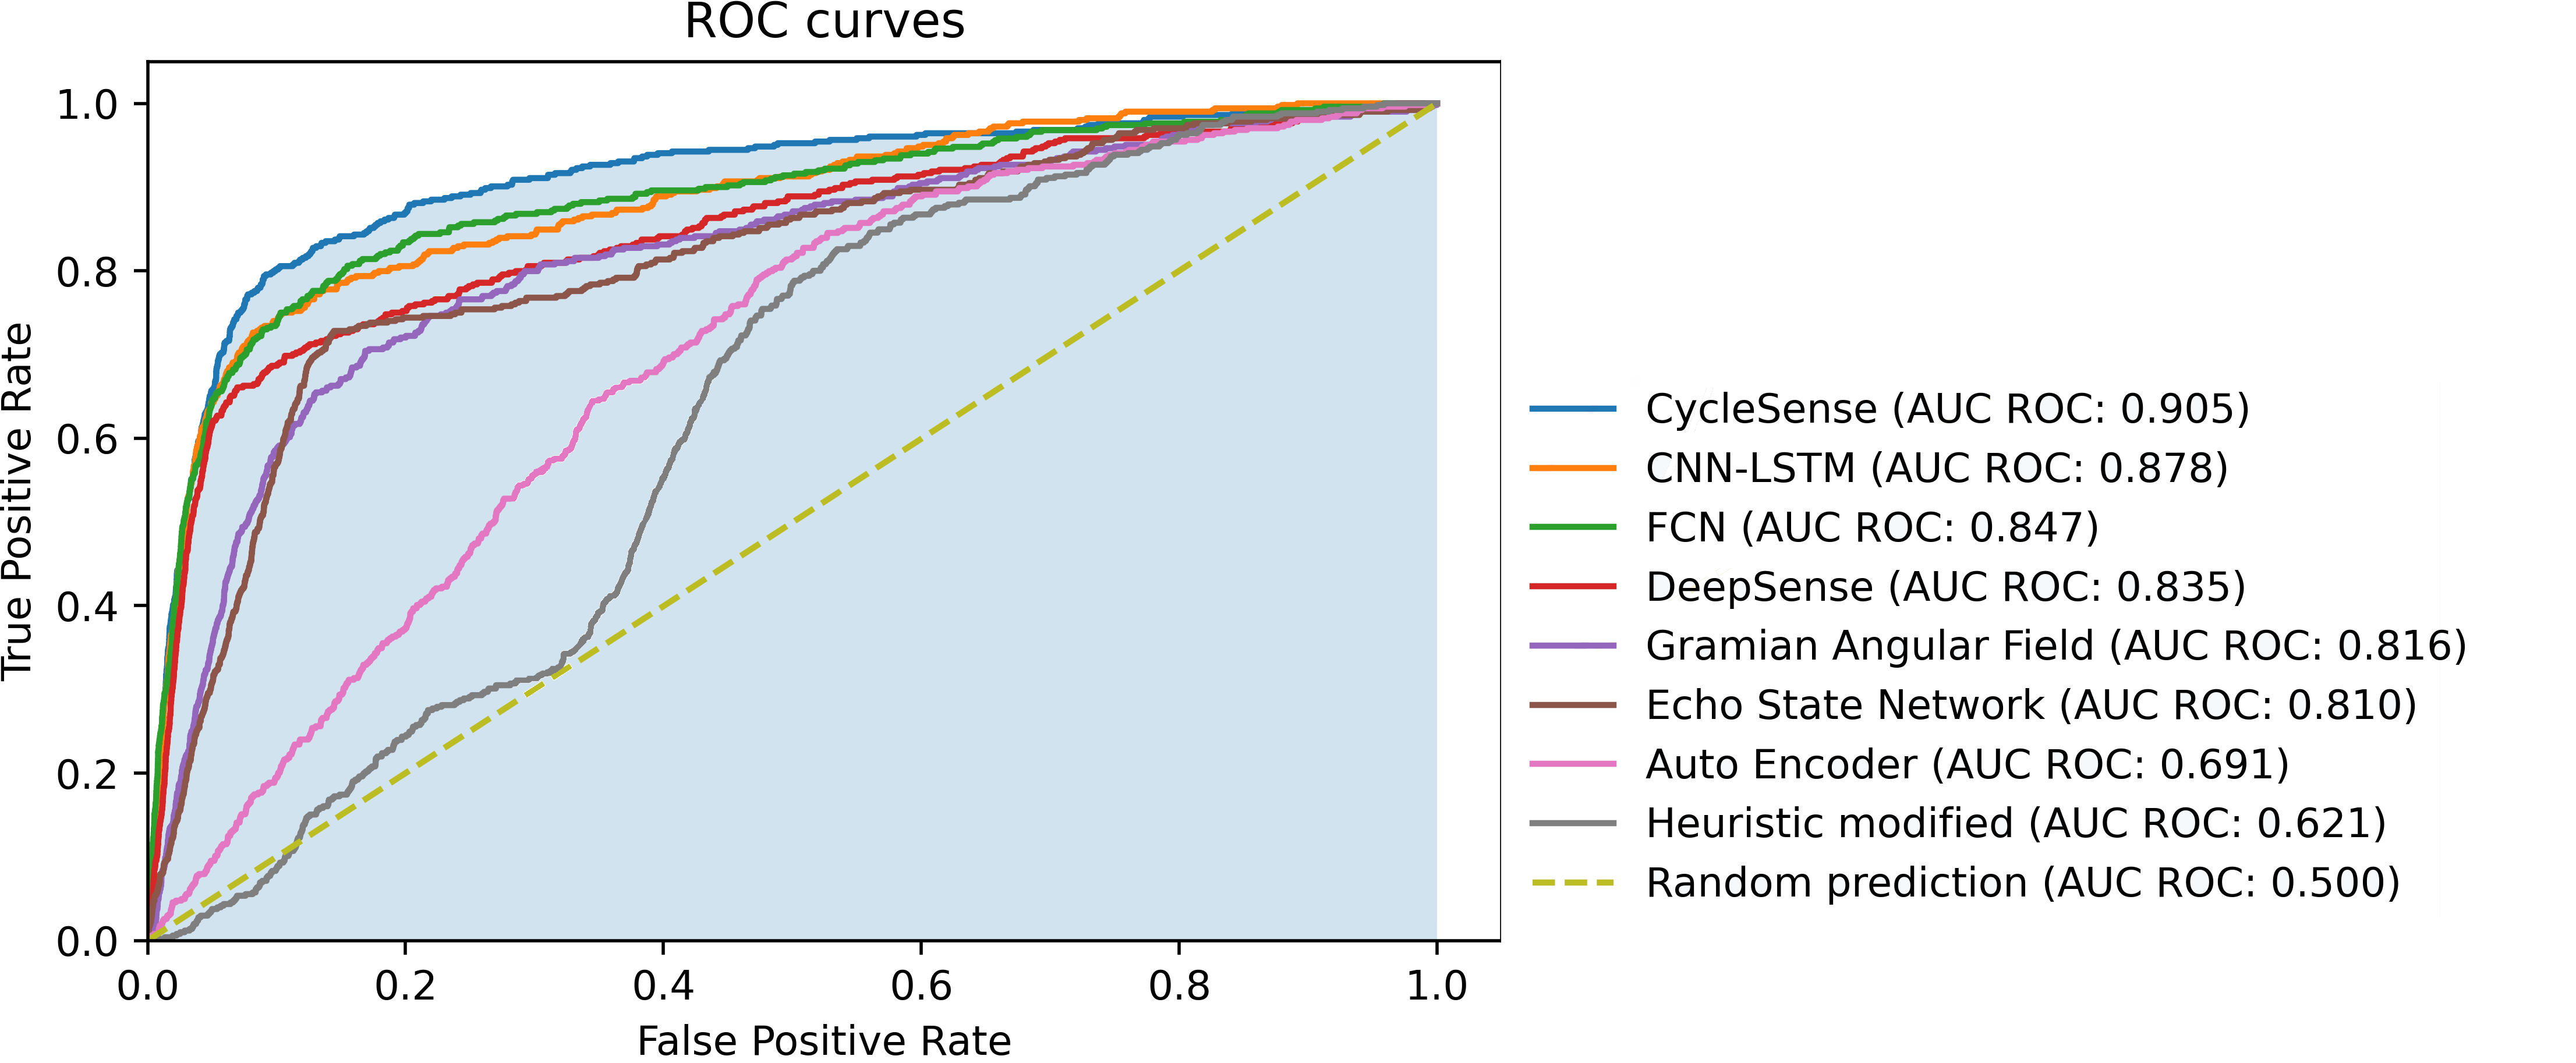
\includegraphics[width=0.8\textwidth]{fig/roc_auc_results_legend.png}
	\caption{Comparison of the baselines and common model architectures used in the context of \ac{dl} for \ac{tsc}~\cite{ismail2019deep} with the CycleSense model. Note that all of these models have been trained and evaluated on rides contained in the SimRa data set that have been recorded with more recent versions of the SimRa Android app.}
	\label{fig:roc-auc-results}
\end{figure}

\begin{table}
	\centering
	\resizebox{\columnwidth}{!}{%
	\begin{tabular}{cccccccccc}
		\hline
		\centering
		& \textbf{TN} & \textbf{FP} & \textbf{FN} & \textbf{TP} & \textbf{\ac{auc} \ac{roc}} & \textbf{Precision} & \textbf{Recall} & \textbf{F1-Score} & \textbf{MCC} \\
		\hline\hline
		\textbf{CycleSense} & 107934 & 10893 & 104 & 400 & \cellcolor{yellow}0.906 & \cellcolor{yellow}0.035 & 0.794 & \cellcolor{yellow}0.068 & \cellcolor{yellow}0.156 \\
		\hline
		\textbf{CNN-LSTM} & 106427 & 12400 & 127 & 377 & 0.878 & 0.030 & 0.748 & 0.057 & 0.135 \\
		\hline
		\textbf{FCN} & 100932 & 18500 & 98 & 402 & 0.847 & 0.021 & \cellcolor{yellow}0.804 & 0.041 & 0.115 \\
		\hline
		\textbf{DeepSense} & 106192 & 12635 & 153 & 351 & 0.835 & 0.027 & 0.696 & 0.052 &  0.123 \\
		\hline
		\textbf{GAF} & 98782 & 20045 & 150 & 354 & 0.816 & 0.017 & 0.702 & 0.034 & 0.092 \\
		\hline
		\textbf{ESN} & 101670 & 17157 & 138 & 366 & 0.810 & 0.021 & 0.726 & 0.041 & 0.107 \\
		\hline
		\textbf{Auto Encoder} & 58416 & 60411 & 88 & 416 & 0.691 & 0.007 & 0.825 & 0.014 & 0.041 \\
		\hline
	\end{tabular}%
}
\caption{Comparison of the baselines and common model architectures used in the context of \ac{dl} for \ac{tsc}~\cite{ismail2019deep} with the CycleSense model. See the discussion in Section~\ref{subsec:metrics} about the usefulness of various metrics. Note also that all of these models have been trained and evaluated on rides contained in the SimRa data set that have been recorded with more recent versions of the SimRa Android app. For all models the threshold which optimizes Youden's index\cite{youden1950index} were chosen.}
\label{tab:roc-auc-results}
\end{table}

In another experiment, we include the linear accelerometer sensor values in addition to the accelerometer, gyroscope and \ac{gps} data we used so far.
The result for CycleSense is again an \ac{auc} \ac{roc} of 0.906, although the model requires more memory, training and processing time.
Therefore, we leave out the linear accelerometer feature.

So far, we have predominantly focused on newer rides recorded on the Android version of the SimRa app.
As shown in Figure~\ref{fig:traindonone}, the model performs far worse on the other splits of the data set.
Therefore, it was necessary to train an individual model for each part of the data set. 
This yields far better results (Figure~\ref{fig:individually}).

\begin{figure}[t]
	\centering
	\begin{subfigure}[b]{0.475\textwidth}
		\centering
		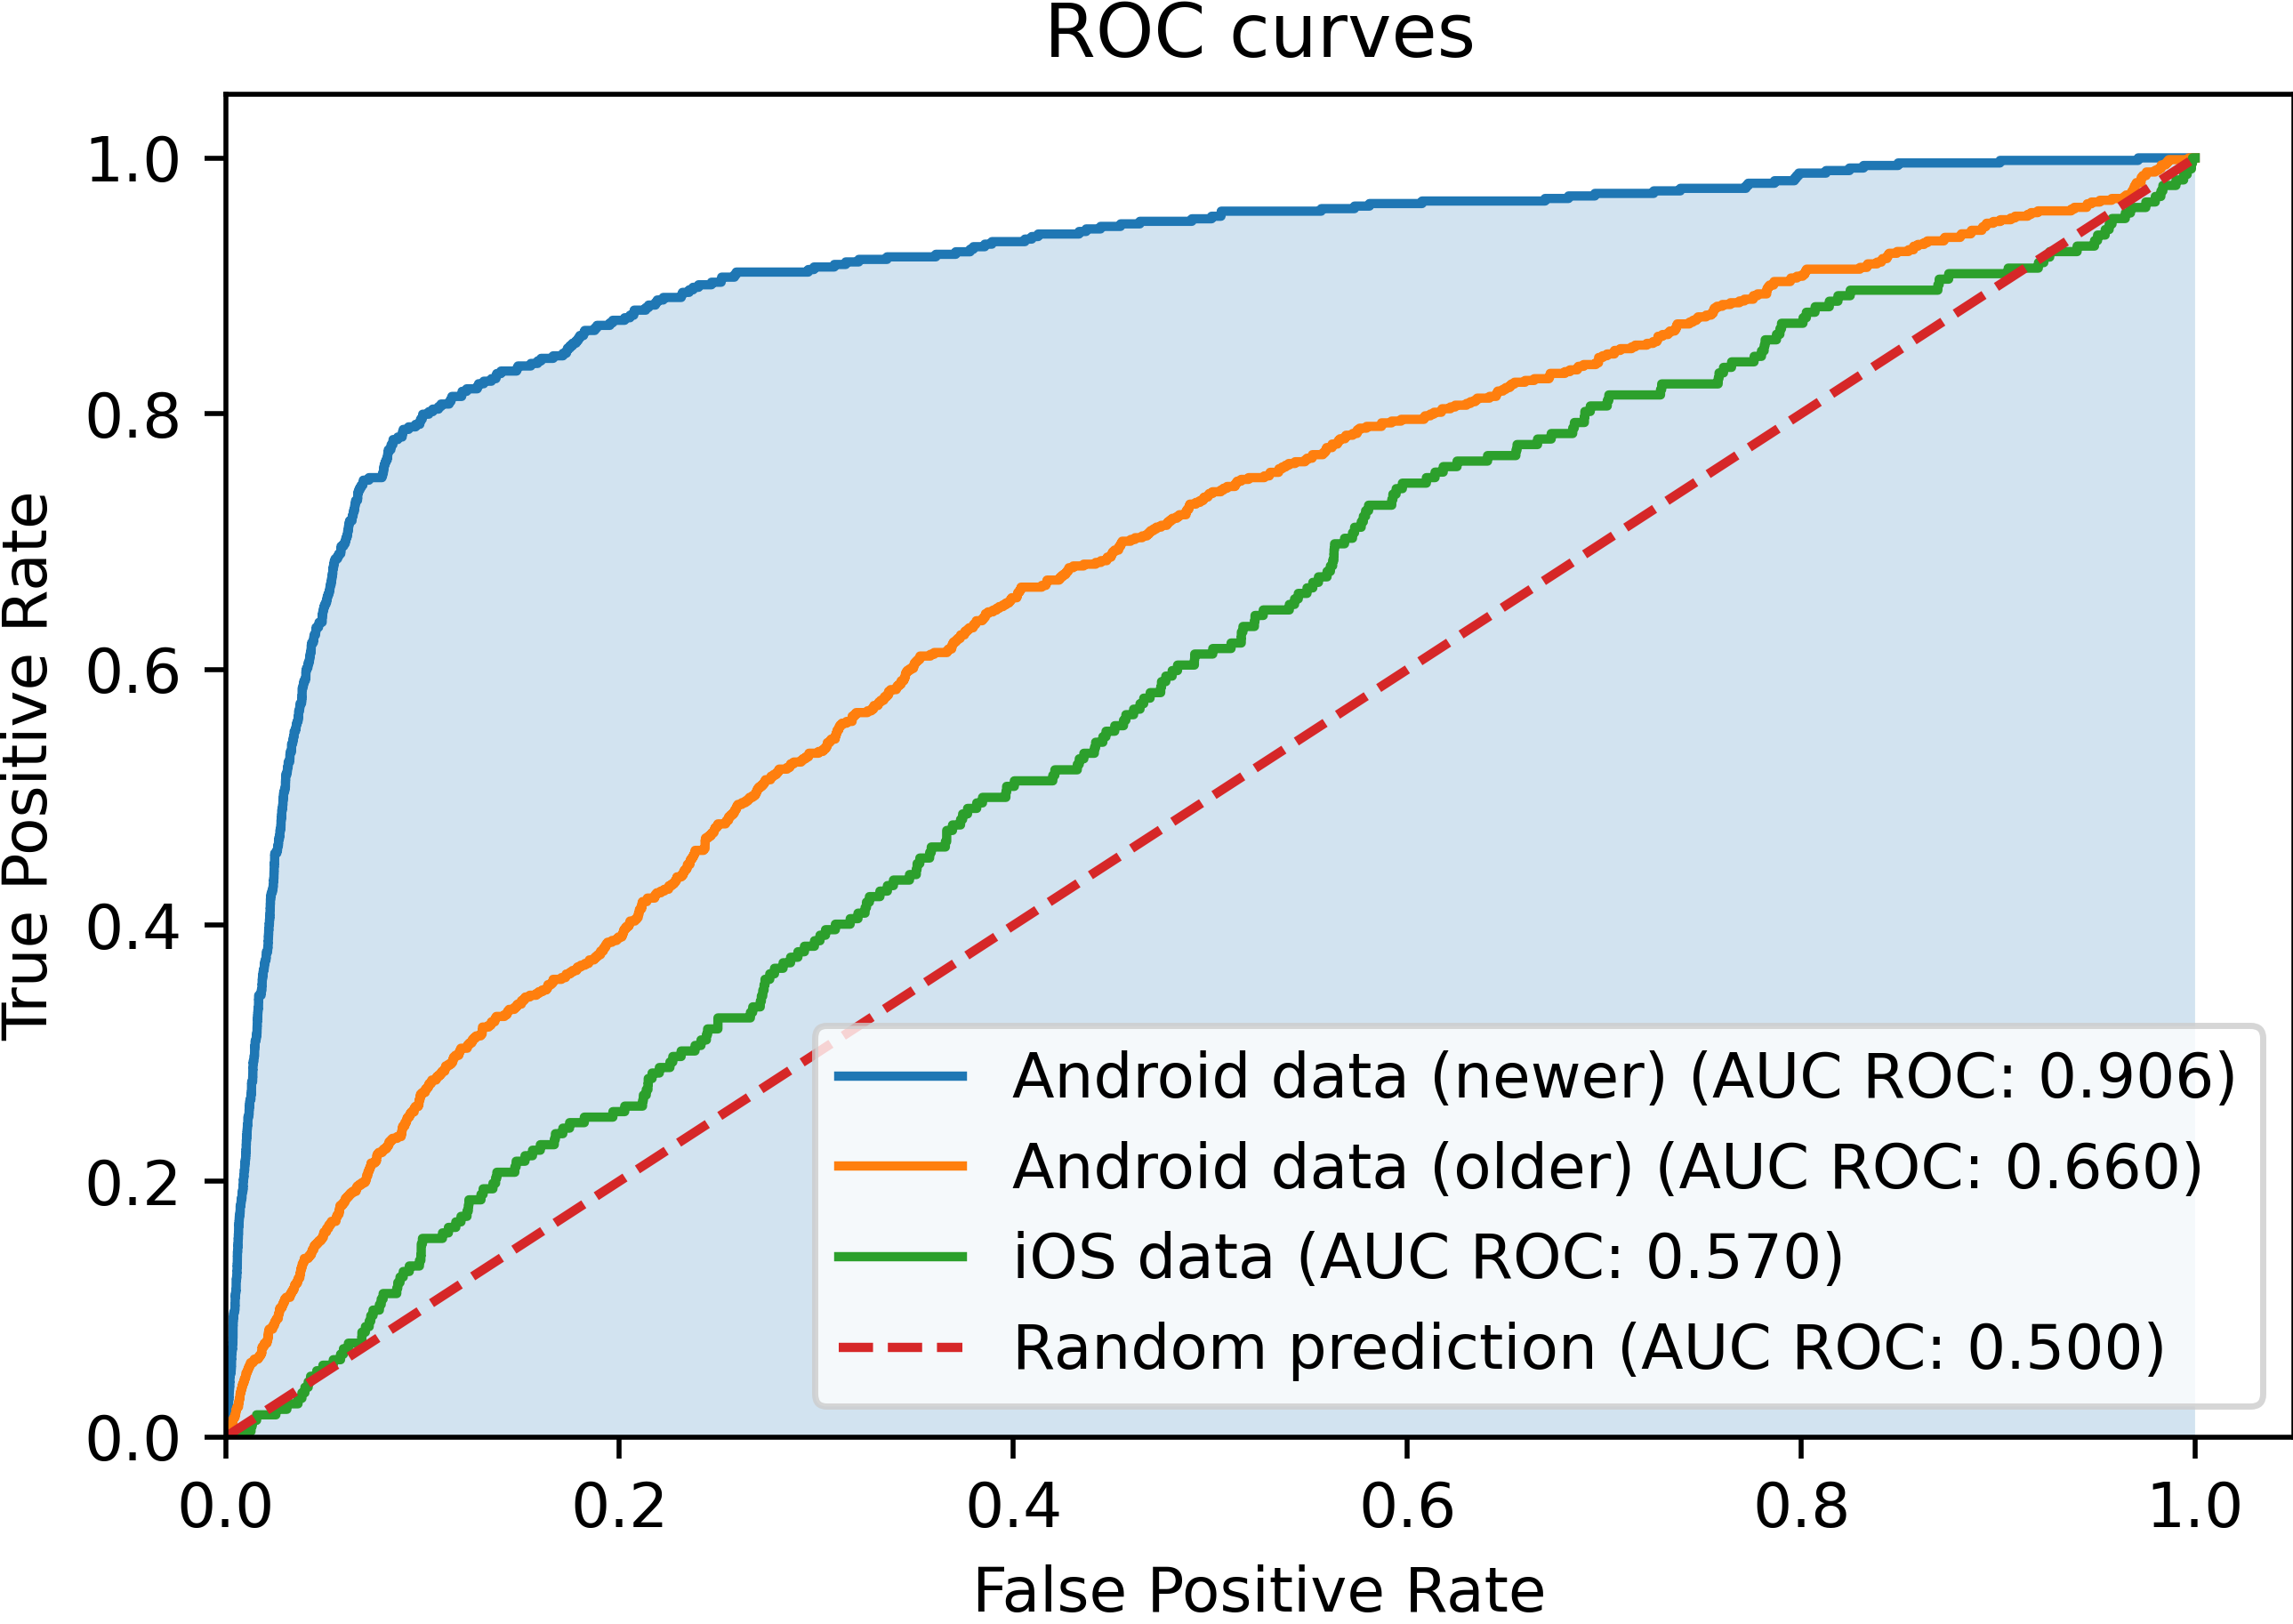
\includegraphics[width=\textwidth]{fig/rocauctrainedon73.png}
		\caption{\small CycleSense trained only on the newer Android rides and evaluated on all parts of the data set.}
		\label{fig:traindonone}
	\end{subfigure}
	\hfill
	\begin{subfigure}[b]{0.475\textwidth}
		\centering
		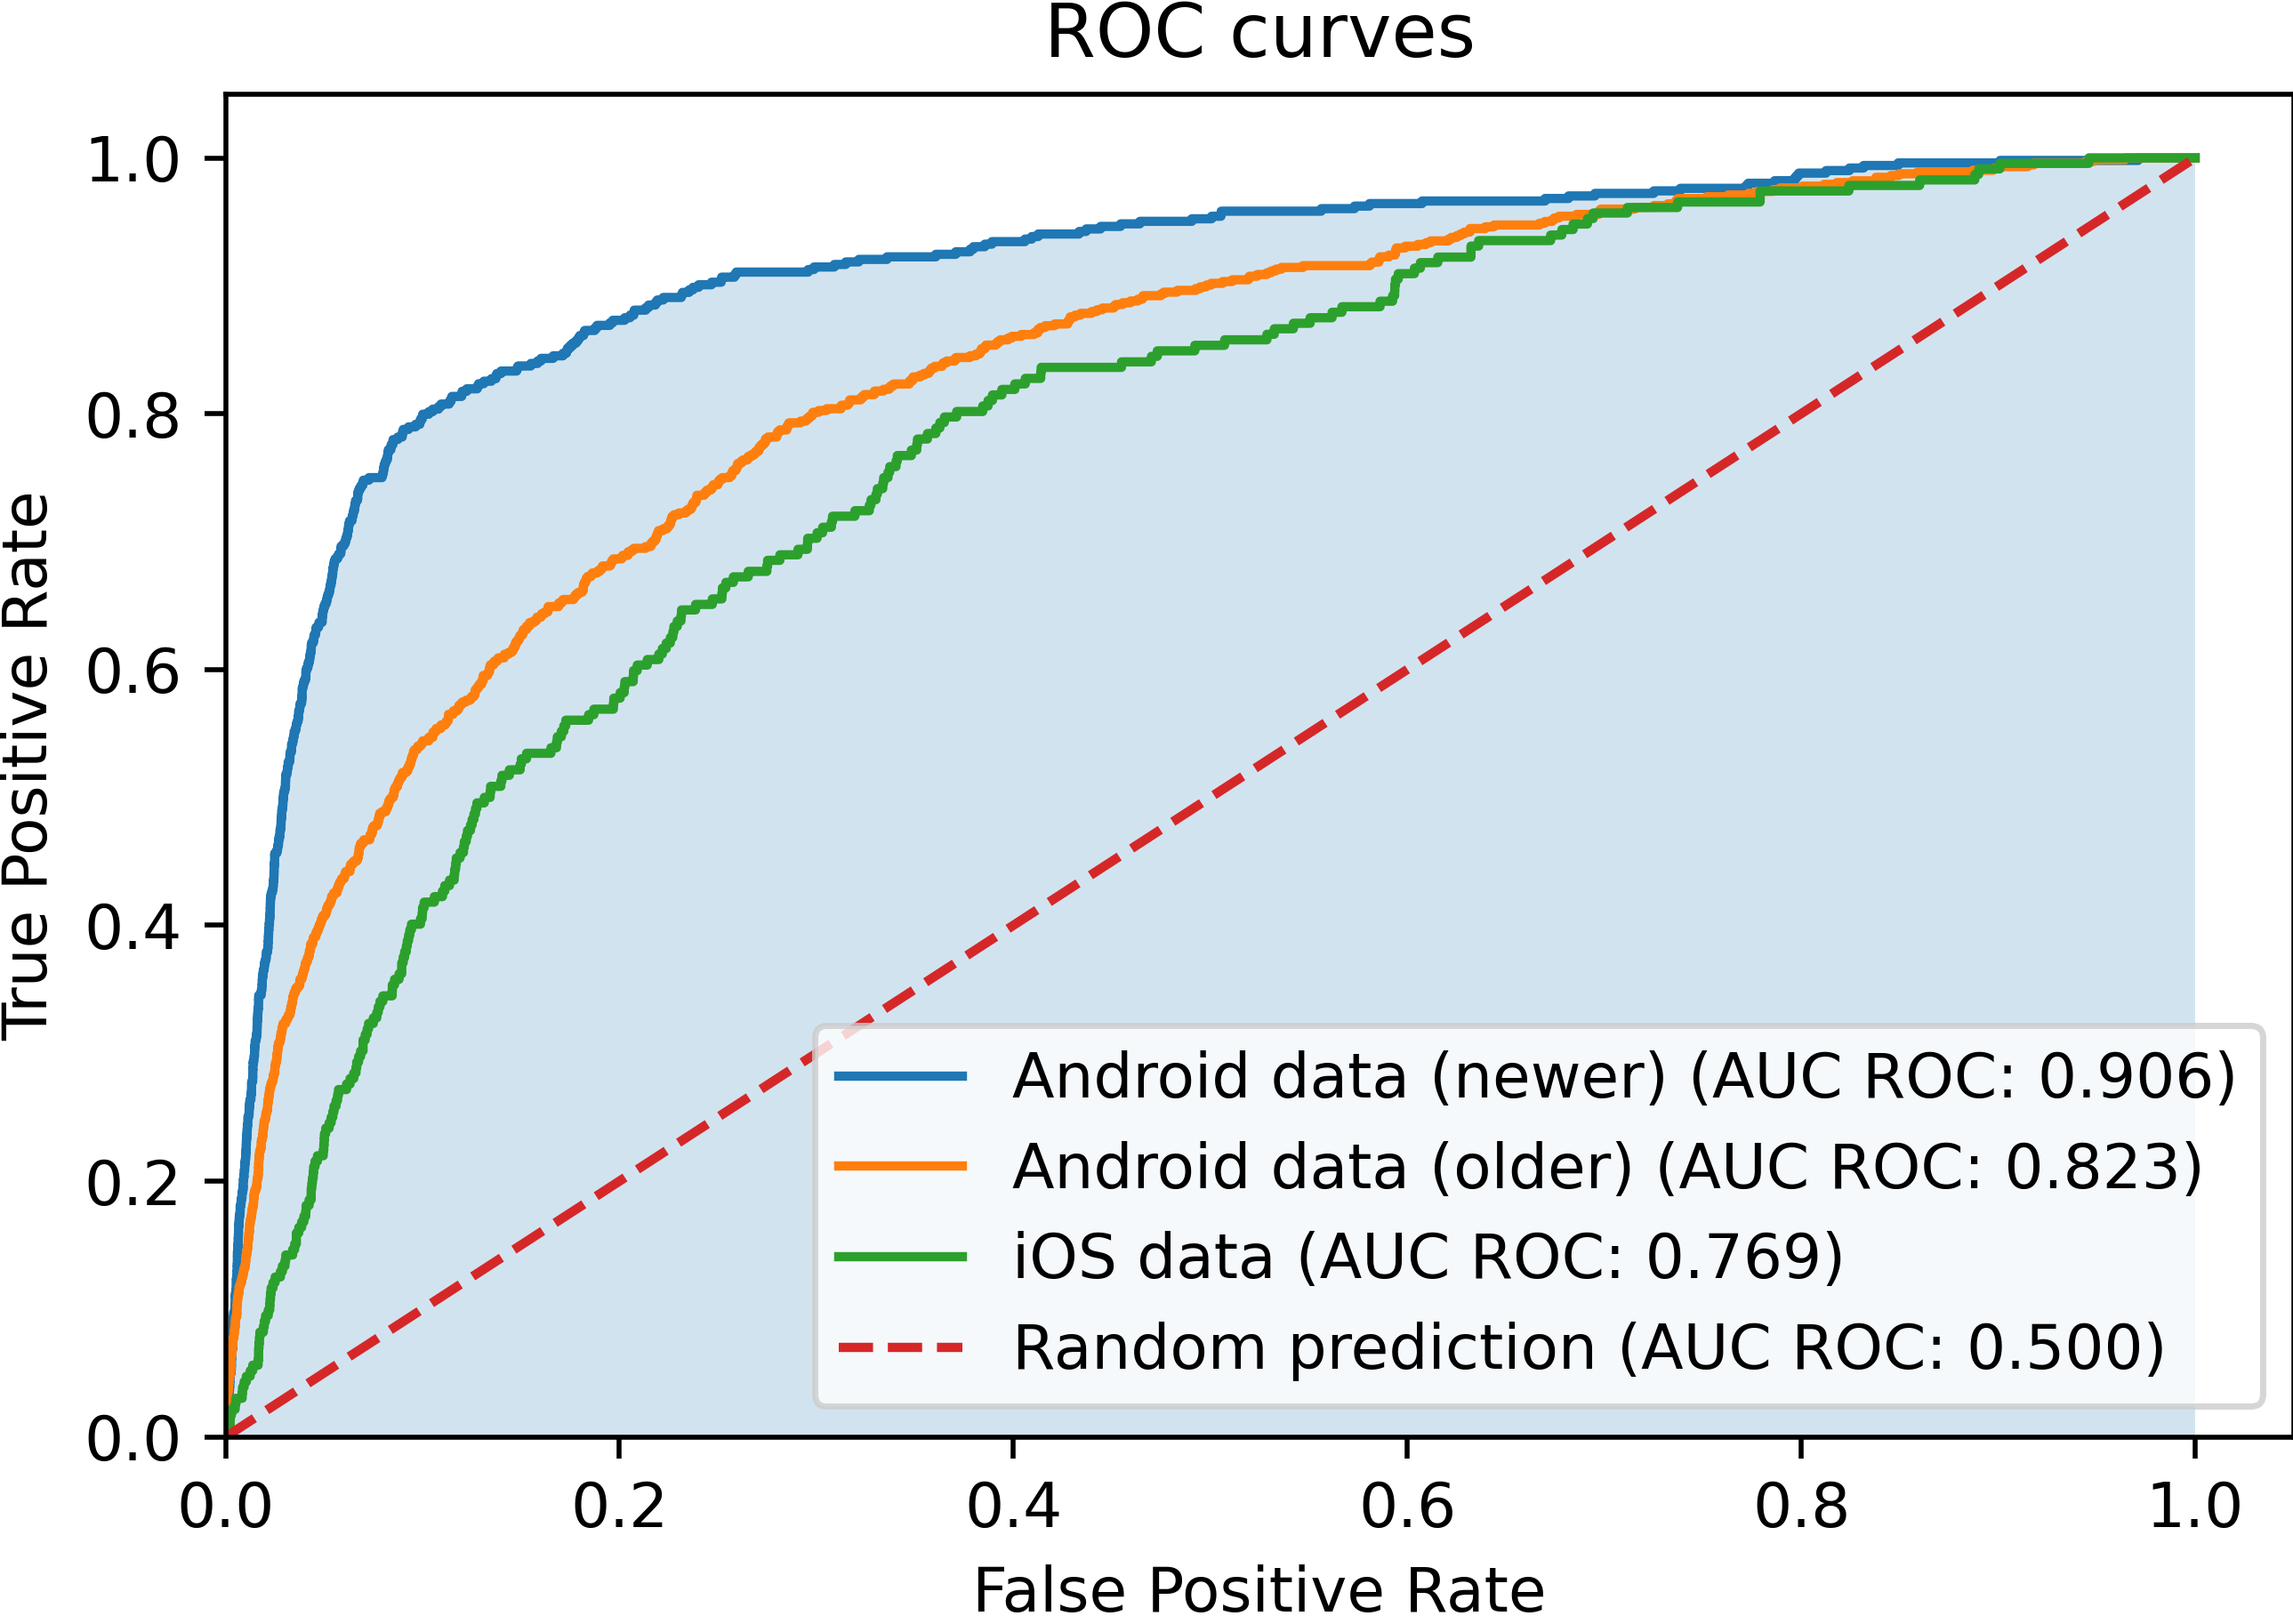
\includegraphics[width=\textwidth]{fig/rocauctrainedindividually.png}
		\caption{\small CycleSense trained and evaluated individually on all parts of the data set. \newline}
		\label{fig:individually}
	\end{subfigure}
	\caption{Comparison of CycleSense trained only on the newer Android rides or individual CycleSense models trained for each part of the data set. Note that only the newer Android data set was manually cleaned.}
	\label{fig:comp-trainedonone-individually}
\end{figure}

As the Berlin region has by far recorded the most rides, we have so far used only those for tuning, training, and evaluating our model.
The SimRa app, however, is deployed in many more regions, so our model is clearly required to perform there, too.
For this reason, we have evaluated the Berlin CycleSense model on the newer Android rides coming from Hanover and Nuremberg.

The outcome of this experiment is visualized in Figure~\ref{fig:different-city-trained-on-berlin}.
It clearly shows, that CycleSense does not perform as good as in Berlin.
Since most regions lack training data, it would not be a feasible solution to train models individually per region in the current stage of the SimRa project.
Instead, we retrain CycleSense on a data set that includes all the rides recorded on the newer versions of the Android app within the Berlin, Nuremberg, and Hanover regions.
The results from Figure~\ref{fig:different-city-trained-individually} show that this clearly improves the performance in these additional regions.
At the same time, the performance on the Berlin data set has declined only slightly (0.029 \ac{auc} \ac{roc}) by comparison.
Nevertheless, the \ac{auc} \ac{roc} for Berlin is still the highest and clearly above Nuremberg, which is well ahead of Hanover.

\begin{figure}[t]
	\centering
	\begin{subfigure}[b]{0.475\textwidth}
		\centering
		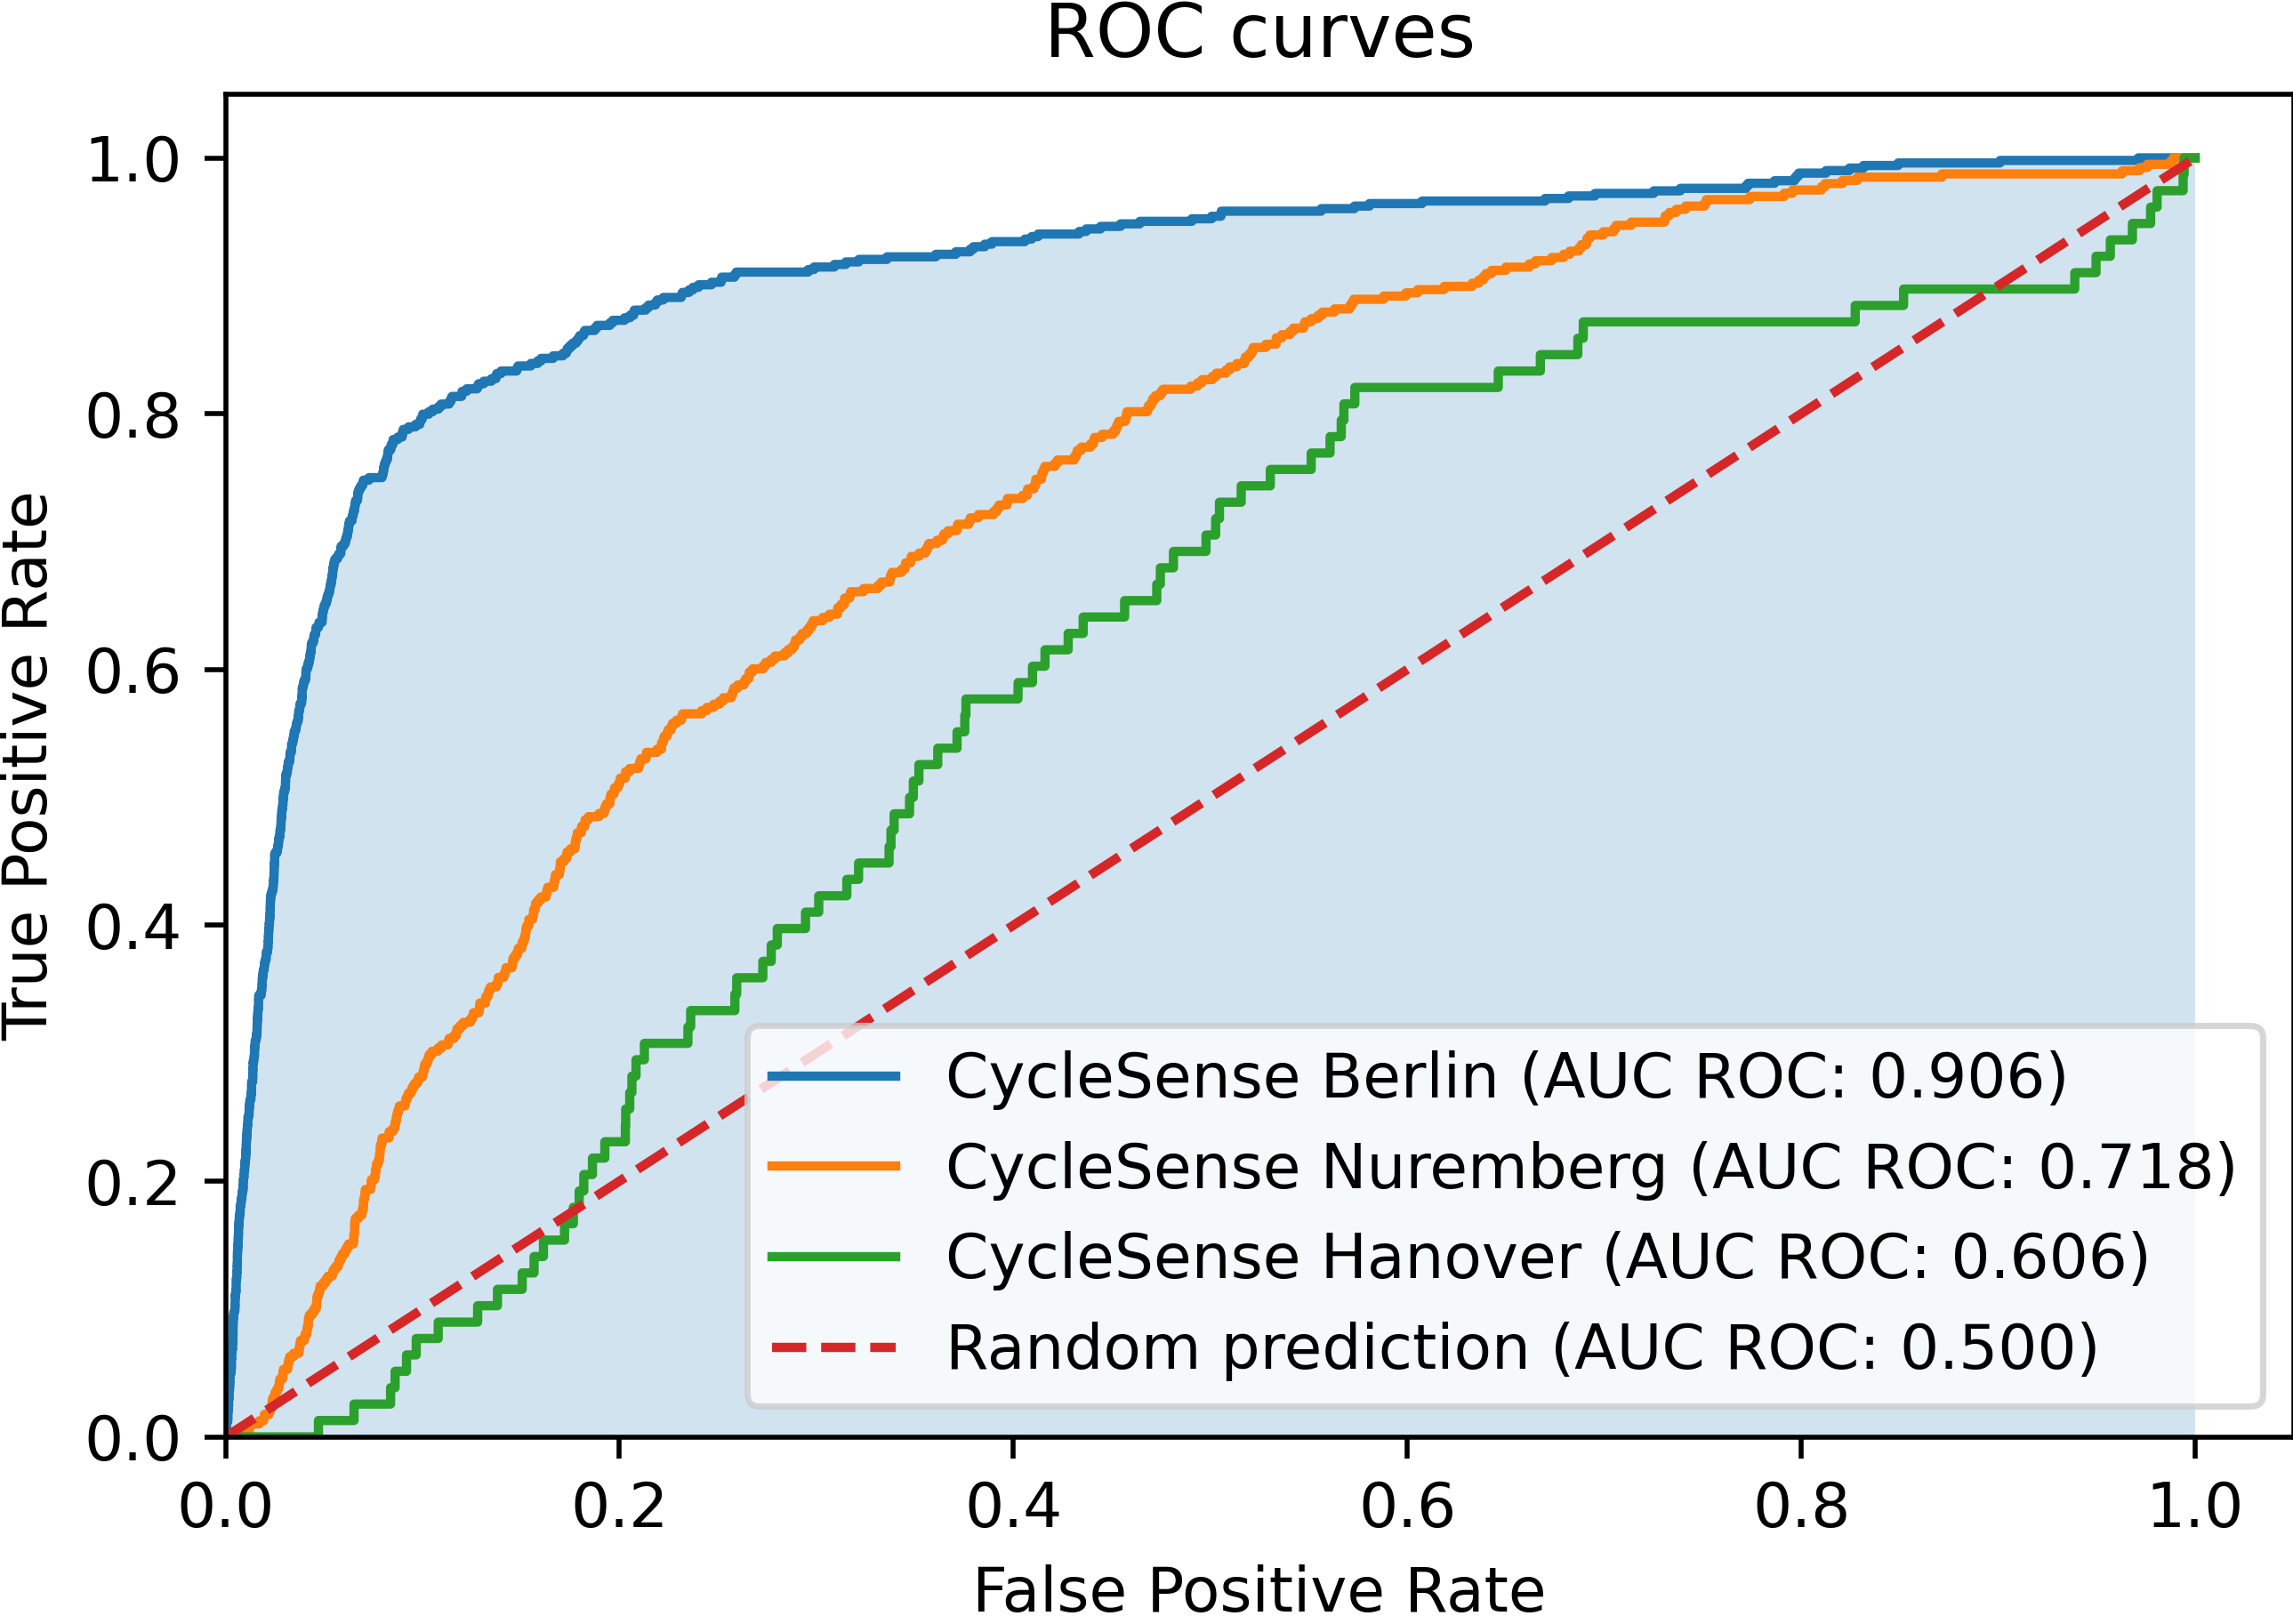
\includegraphics[width=\textwidth]{fig/city_comp_before.png}
		\caption{\small Performance of CycleSense trained on the new Android data set of rides recorded in Berlin. \newline}
		\label{fig:different-city-trained-on-berlin}
	\end{subfigure}
	\hfill
	\begin{subfigure}[b]{0.475\textwidth}
		\centering
		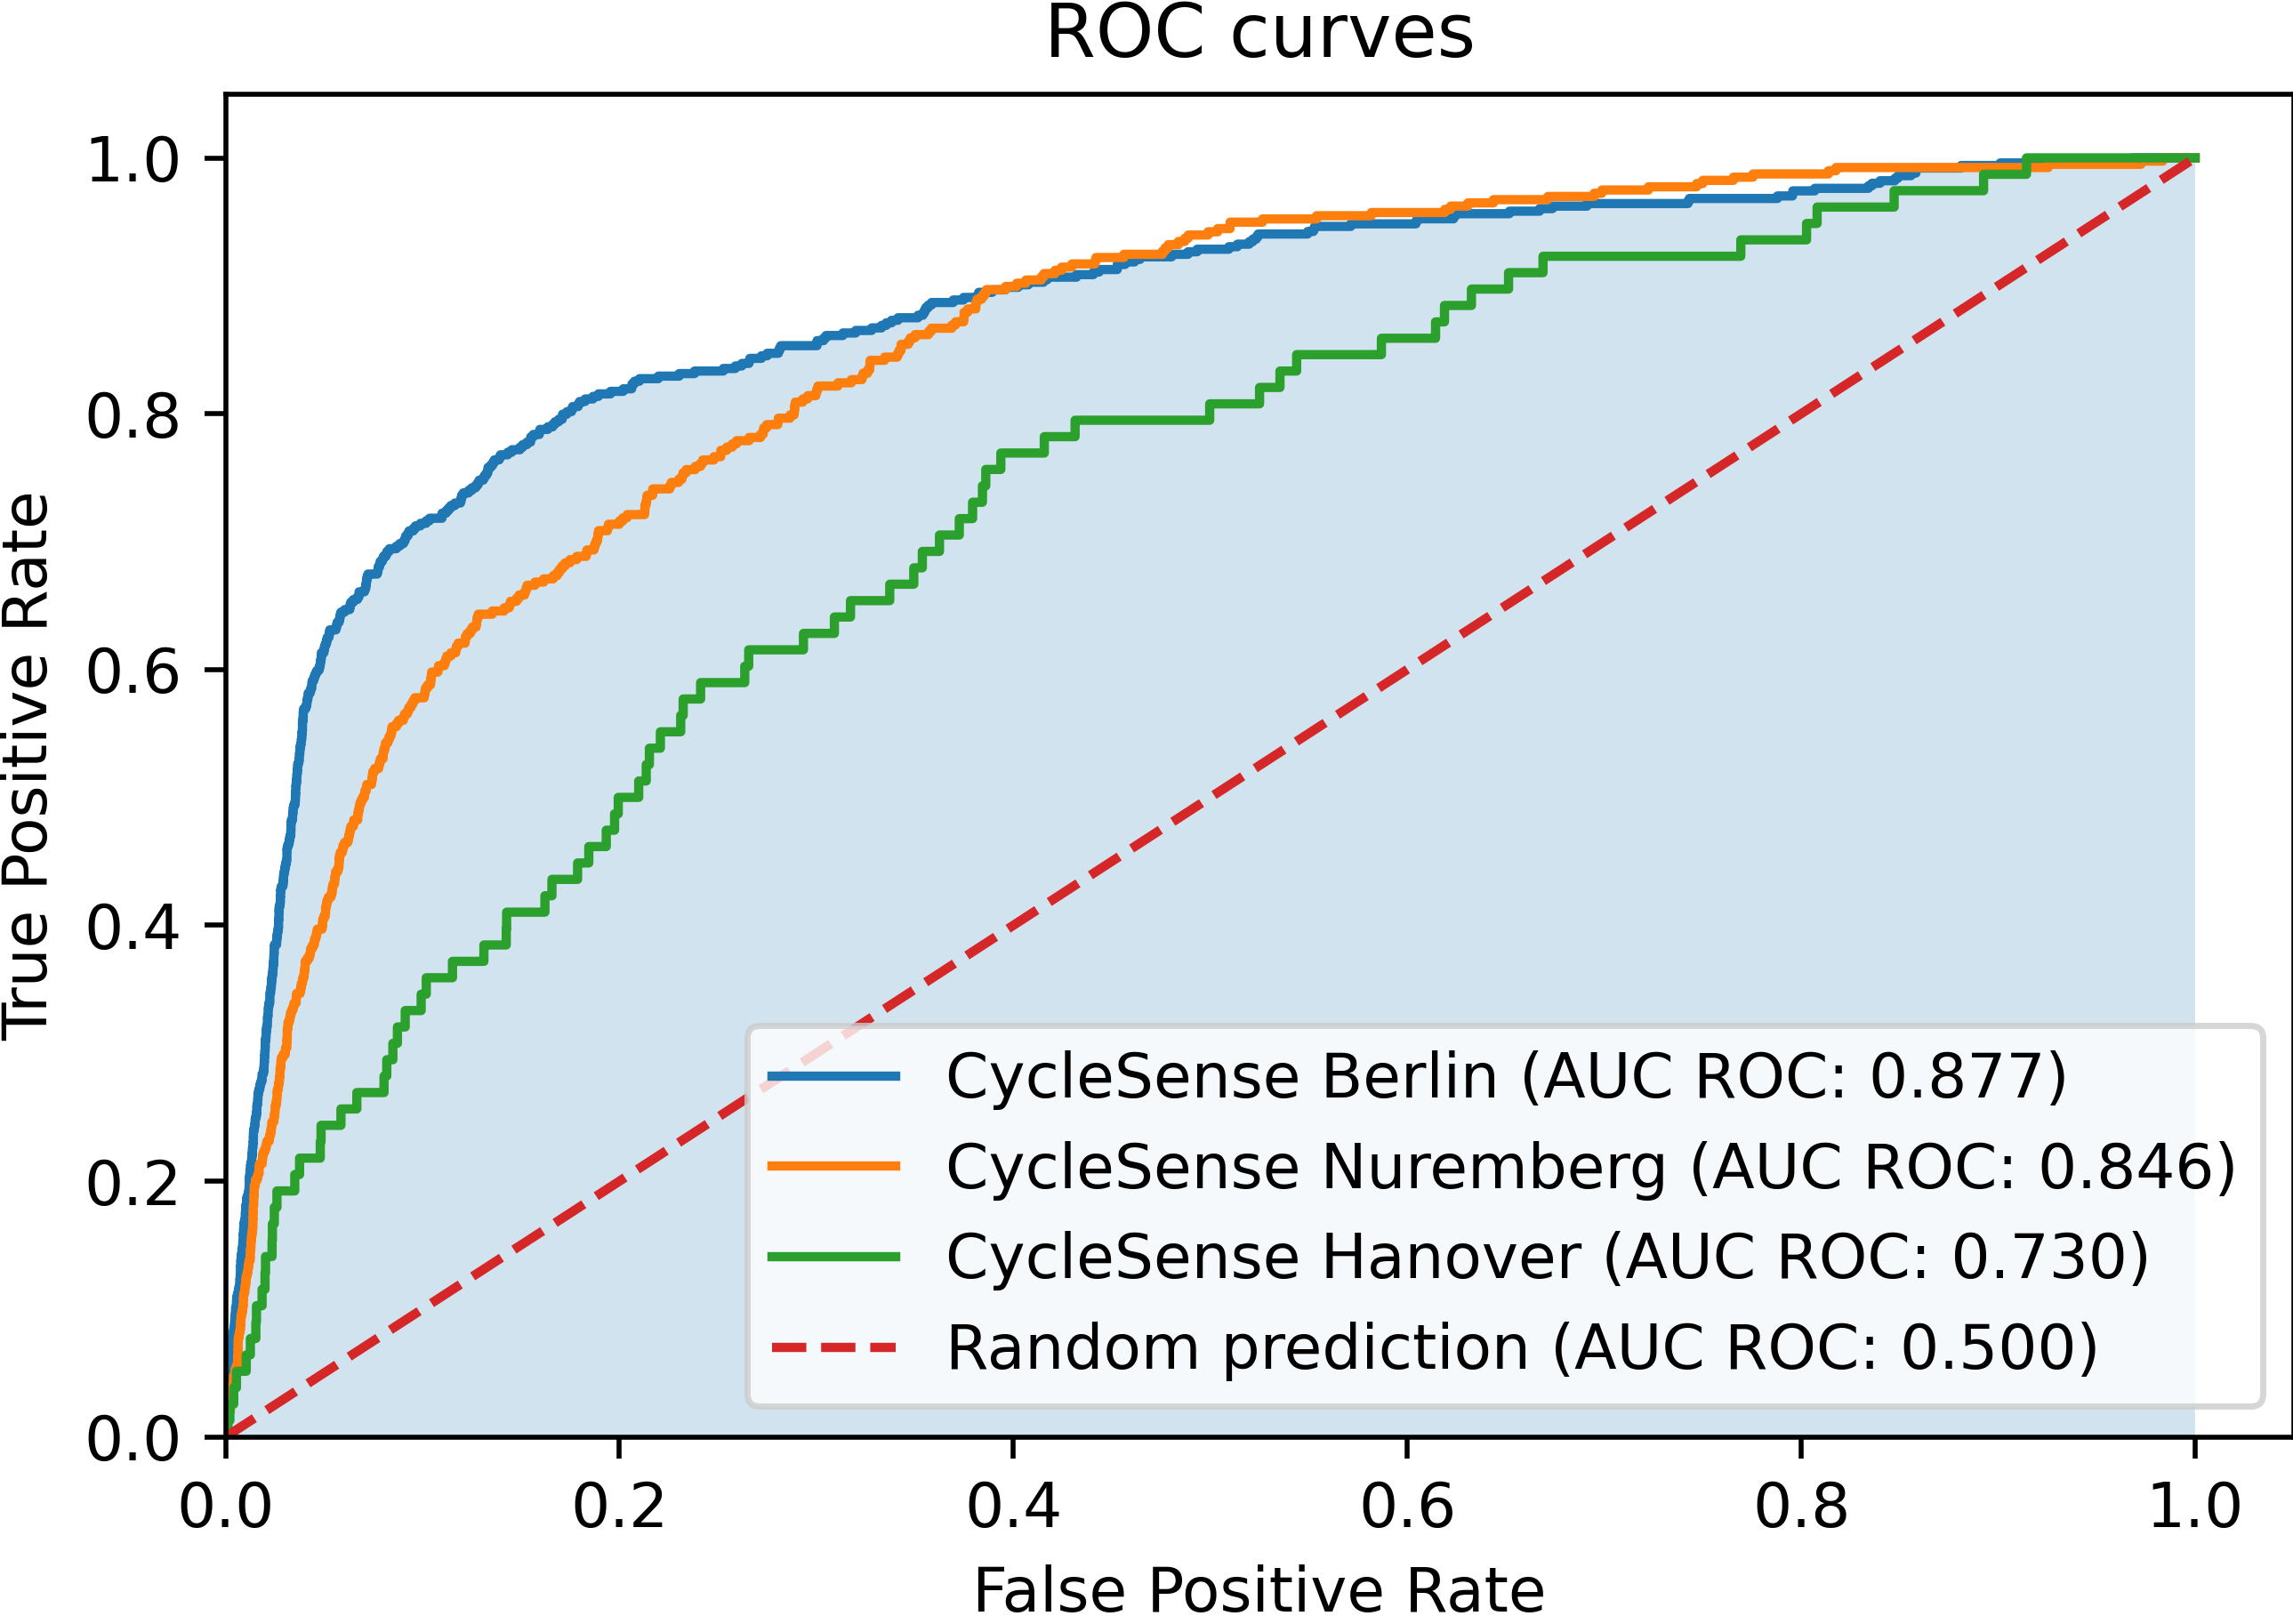
\includegraphics[width=\textwidth]{fig/city_comp_after.png}
		\caption{\small Performance of CycleSense trained on the new Android data set of rides recorded in Berlin, Nuremberg, and Hanover.}
		\label{fig:different-city-trained-individually}
	\end{subfigure}
	\caption{Comparison of the performance of CycleSense trained on Berlin and trained on the other regions combined.}
\end{figure}

\section{Discussion}
\label{sec:discussion_cyclesense}
Our results demonstrate that the proposed CycleSense model outperforms every other model that we have compared to.
While improving the model's architecture and other components, we identified a number of challenges inherent to the problem setting that we discuss in the following.


\subsection{Impact of Preprocessing \& Training Steps}
\label{subsec:impact_of_preprocessing_and_training_steps}
In a first step, we want to highlight the importance of our preprocessing and training methods for the success of our model.
Therefore, Figure~\ref{fig:impact} illustrates the performance of CycleSense when one of the preprocessing or training methods is skipped, resulting in a significant drop in performance in each of the four examples.

\begin{figure}[t]
	\centering
	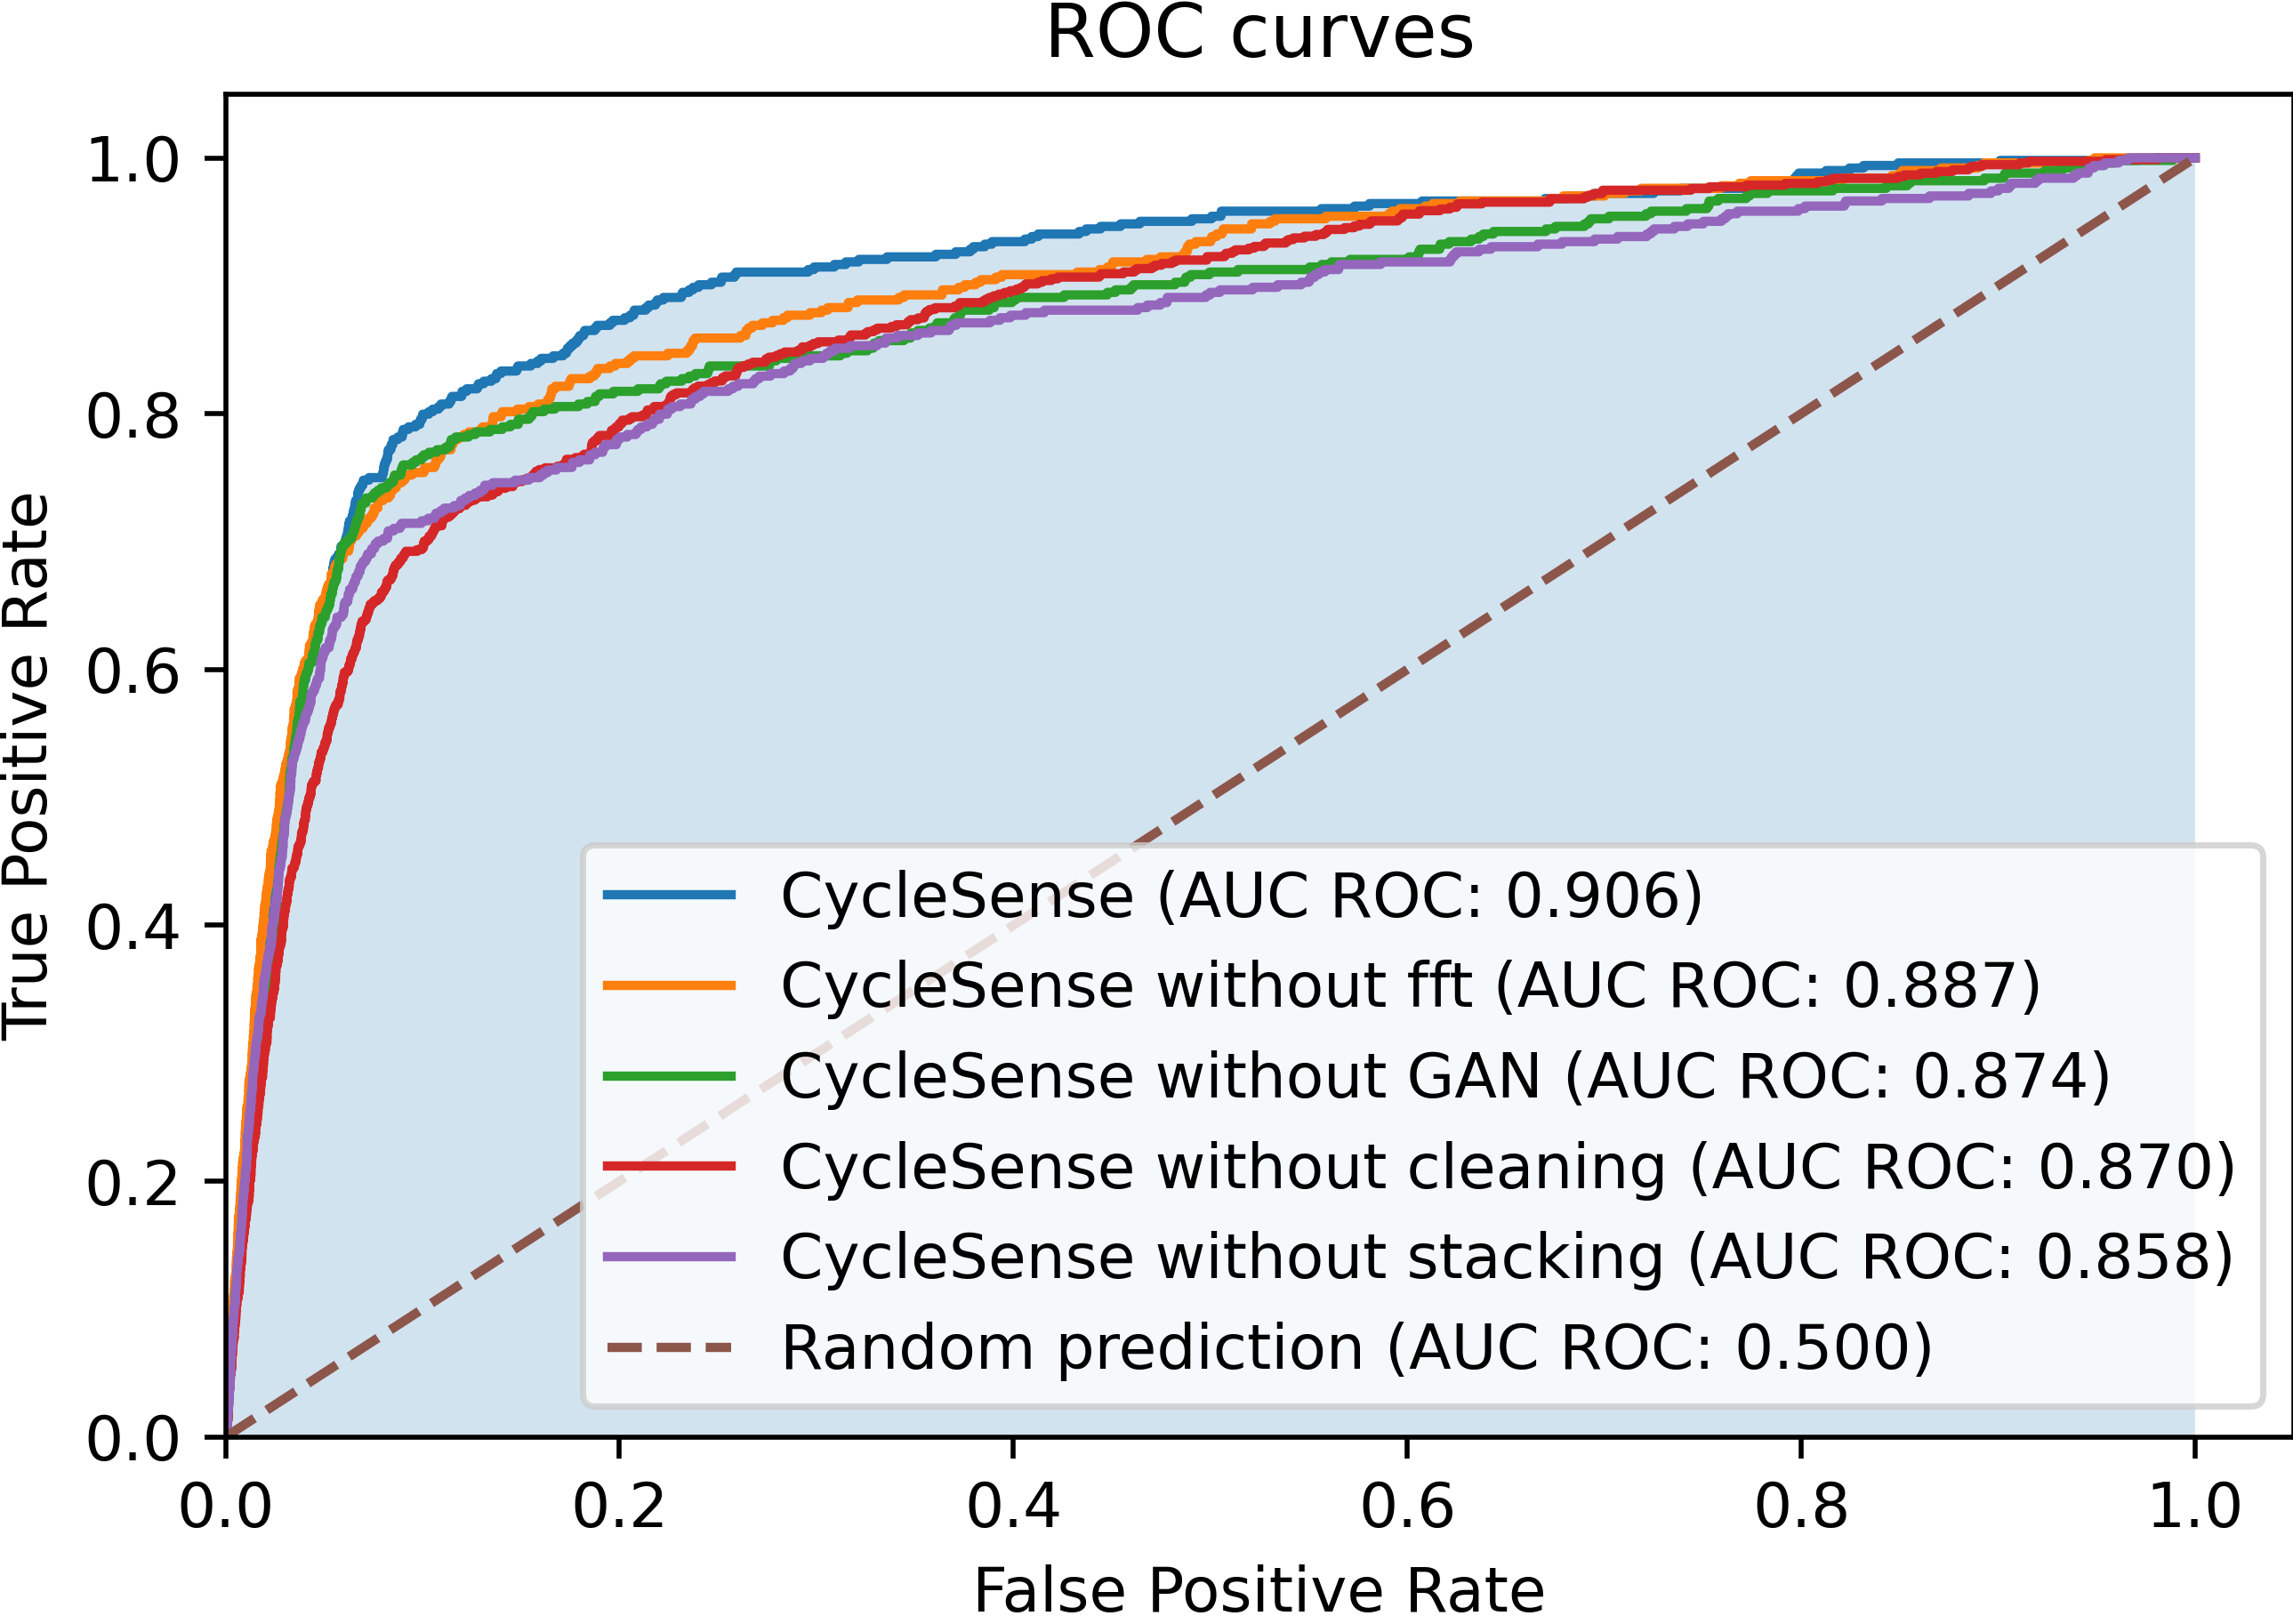
\includegraphics[width=0.5\textwidth]{fig/impact.png}
	\caption{Impact of different preprocessing and training steps on the performance of CycleSense.}
	\label{fig:impact}
\end{figure}

\subsection{Limitations of Crowdsourced Data}
\label{subsec:limitations_of_crowdsourced_data}
Crowdsourced data are generally noisy which could contribute to a reduced model performance.
They do also contain several biases, e.g., the Selection Bias, Device Positioning Bias, Extreme Aversion Bias, or Confirmation Bias~\cite{basiri2019crowdsourced, chakraborty2017makes, kahneman1991anomalies}.
In this context, the heterogeneity across devices and platforms is likely another factor of influence.
As already described, the application that is used by contributors to record their rides is available on two platforms. 
Those platforms are supported by a wide range of different devices and models with different hardware inside. 
Phone manufacturers use different \ac{gps}, gyroscope, and accelerometer sensors that can vary immensely in sensitivity and overall behavior.
Stisen et al.~\cite{stisen2015smart} have shown that there is major heterogeneity when it comes to the accuracy of sensor readings. 
While the main focus of that study was on accelerometer data, Kuhlmann et al.~\cite{kuhlmann2021smartphone} have shown that orientation sensor data is also affected by this variability.
This is in contrast to the \ac{har} tasks, we compare our task to.
The \ac{har} data set~\cite{anguita2013public} was generated under laboratory conditions that always used the same smartphone type body mounted to the exact same position on selected study participants.
This significantly simplifies the classification task.
Another factor that contributes to the issue of noisy crowdsourcing data in the SimRa data set is the fact that some users misinterpret the purpose of the SimRa app.
Instead of labeling incidents, they report, e.g., dangerous areas or annoying traffic lights.
These can of course not be captured by the sensors used.
Many such ``incidents'' can be identified through the comment column of the data set.
It should also be noted that the SimRa data set was not recorded and labeled with the goal of developing ML models -- the goal was to record data which will be analyzed and processed by humans.

\subsection{Technical Limitations of the SimRa Data Set}
\label{subsec:technical_limitations_of_the_simra_data_set}
Recording rates of sensor readings deviate among devices and operating systems and impair model predictions~\cite{stisen2015smart}, this may also affect the performance of CycleSense:
As illustrated in Figure~\ref{fig:emp-measurements}, the recording rates differ significantly in older and newer Android rides as well as in iOS rides.
While the iOS rides' median ($\approx$ 300 ms) is similar to the one of newer Android rides, the \ac{iqr} is much greater and spans approximately 150 ms.
This circumstance could indicate that the relatively weak model performance on this data set can partly be explained by that factor. 
Furthermore, the gyroscope data is recorded with a higher frequency in newer Android rides than in older Android or iOS rides.
This factor could also contribute to the different model evaluation results. 
The achieved \ac{auc} \ac{roc} for uncleaned newer Android data was 0.870, while it was 0.823 for the older Android data.

\begin{figure}[t]
	\centering
	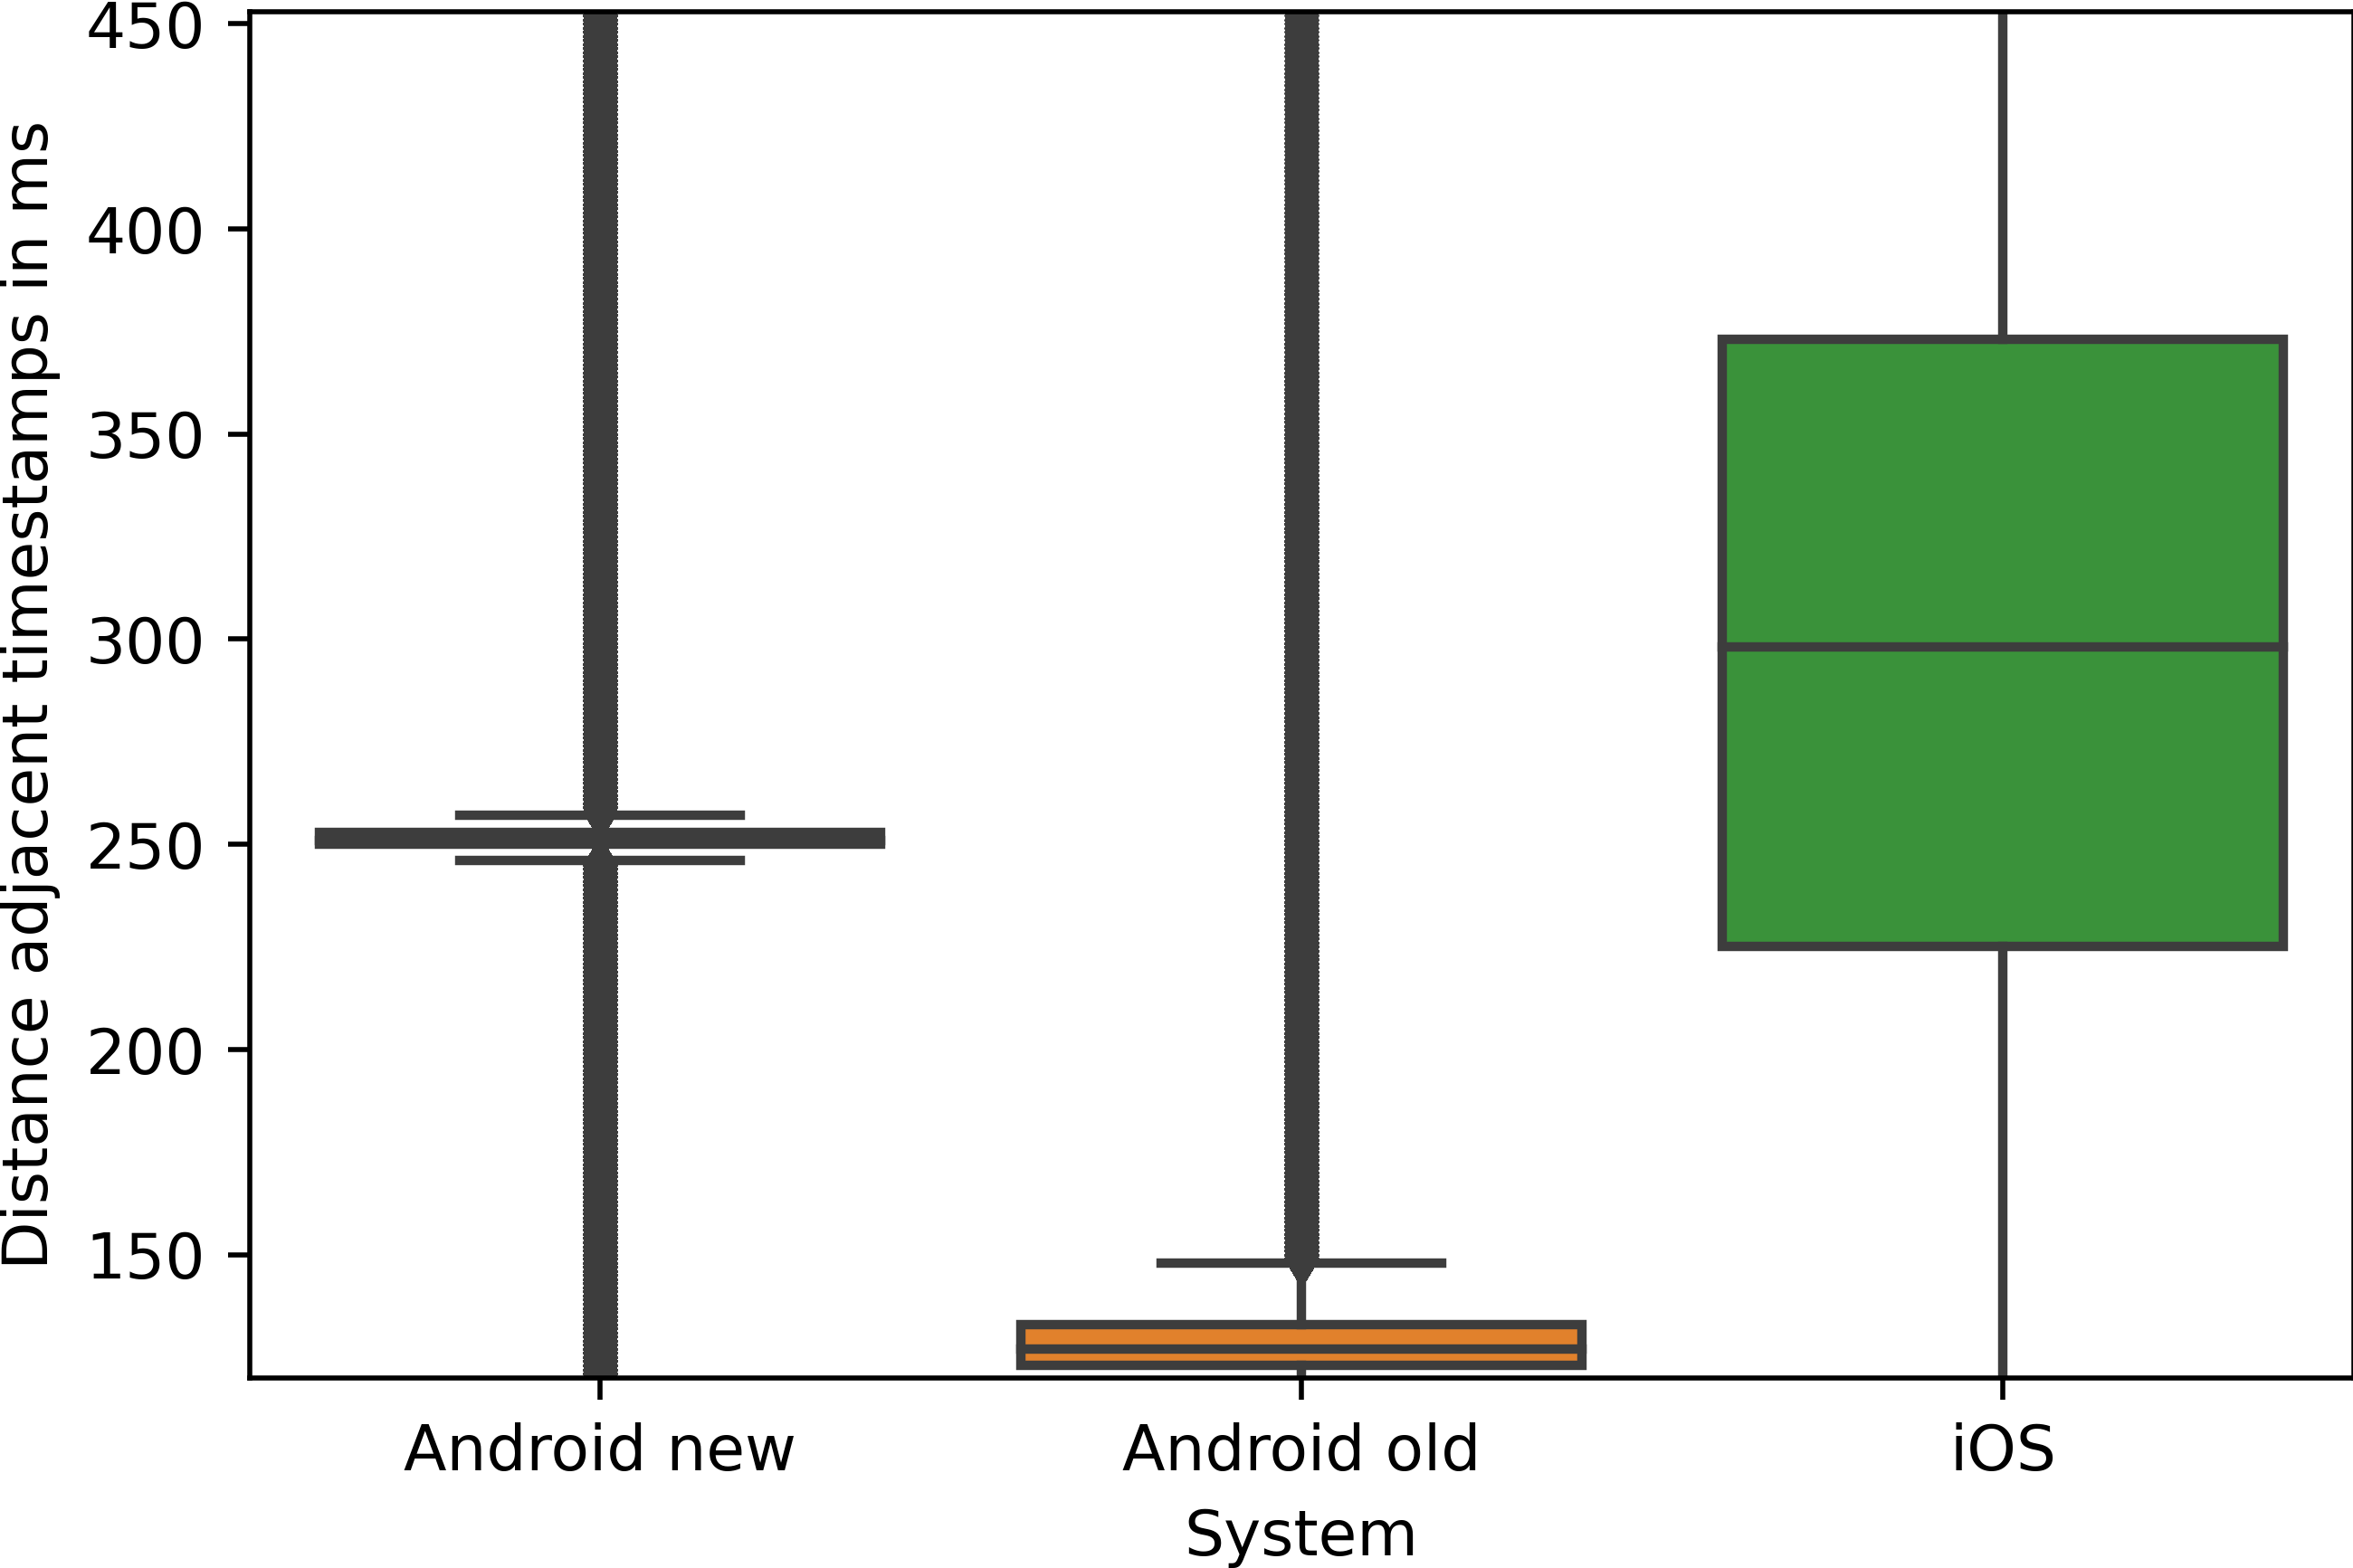
\includegraphics[width=0.45\textwidth]{fig/empirical_measurements.png}
	\caption{Box plot showing the empirical measurement times observed in the SimRa data set for rides recorded with different versions of the SimRa app.}
	\label{fig:emp-measurements}
\end{figure}

Aside from that, the moving average that is used in the SimRa app to condense the data and comply to users' upload volume constraints~\cite{karakaya2020simra} reduces the amplitude and shifts the exact point in time of incidents and other events.
This has the effect that incidents and non-incidents are hard to distinguish as illustrated in Figure~\ref{fig:heavy-vs-normal-braking}.
Both these factors could hurt the model's ability to classify incidents correctly based on the data.
It is important to acknowledge that this issue becomes less severe when the sampling frequency is higher, as it is the case for the older Android data.

\begin{figure}[t]
	\centering
	\begin{subfigure}[b]{0.475\textwidth}
		\centering
		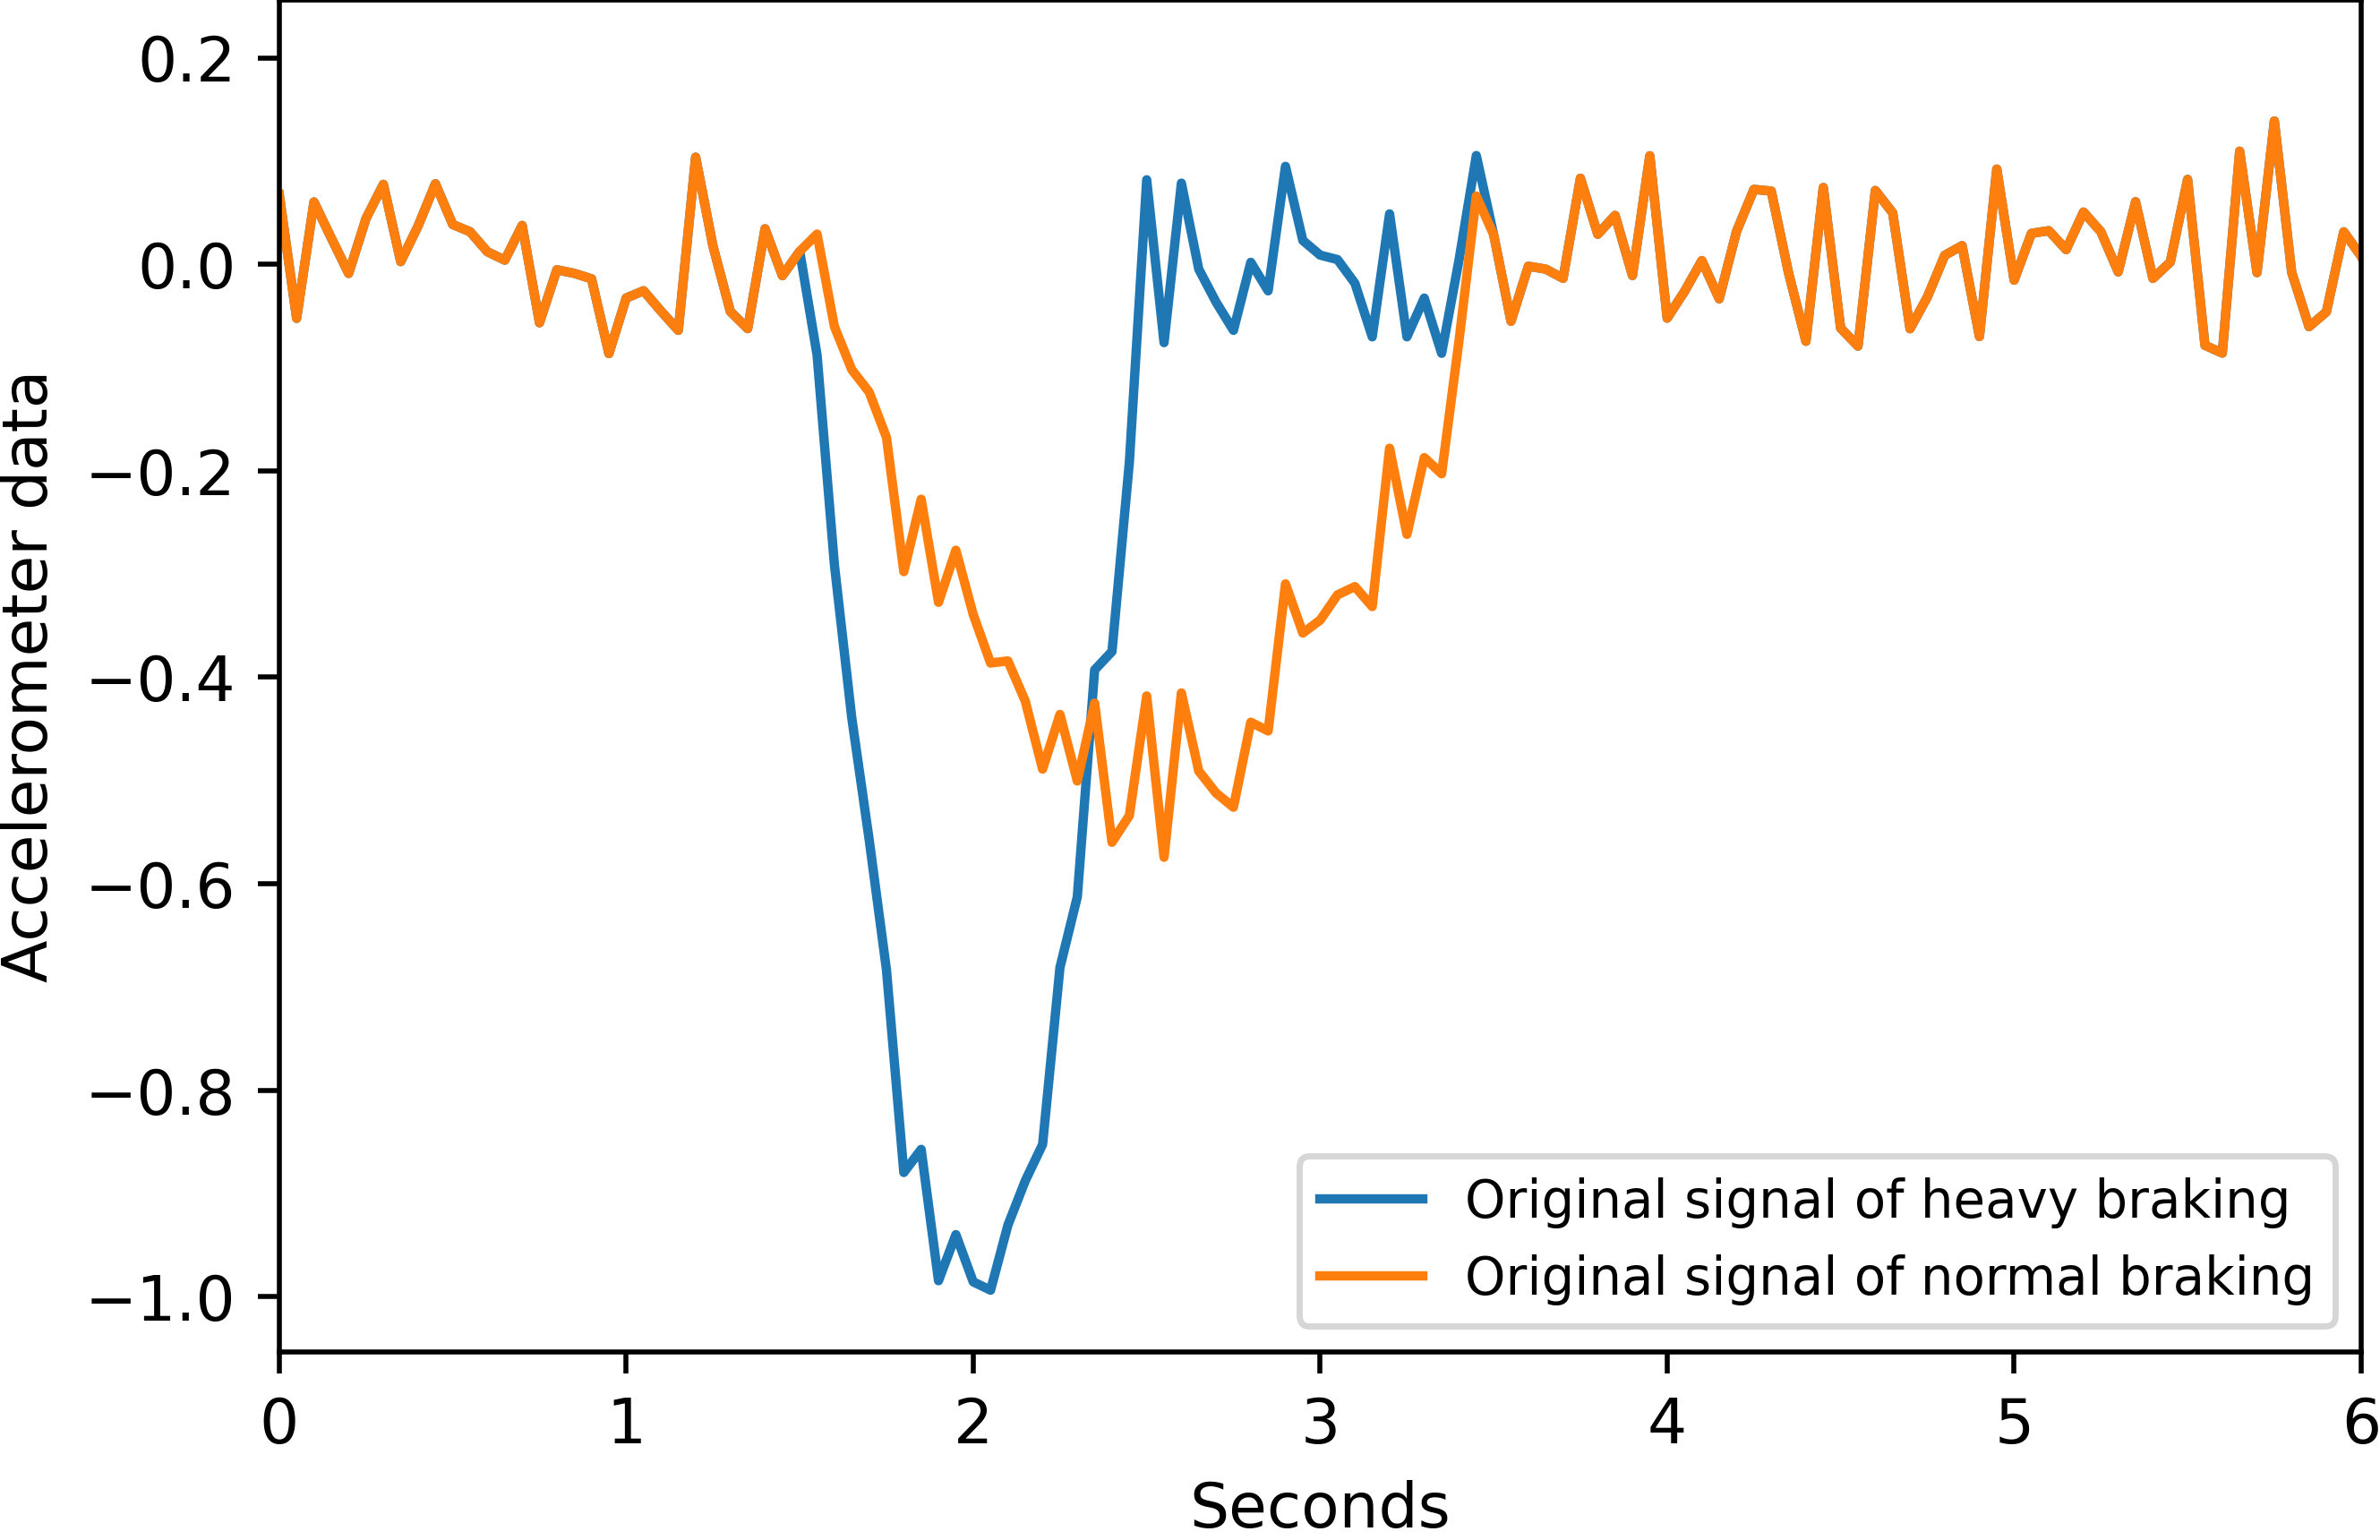
\includegraphics[width=\textwidth]{fig/heavy_vs_normal_braking}
		%\caption{\small Scaled accelerometer data over time of the original signal of an artificially modeled incident with heavy braking vs.\ an artificially modeled moderate braking event.}
	\end{subfigure}
	\hfill
	\begin{subfigure}[b]{0.475\textwidth}
		\centering
		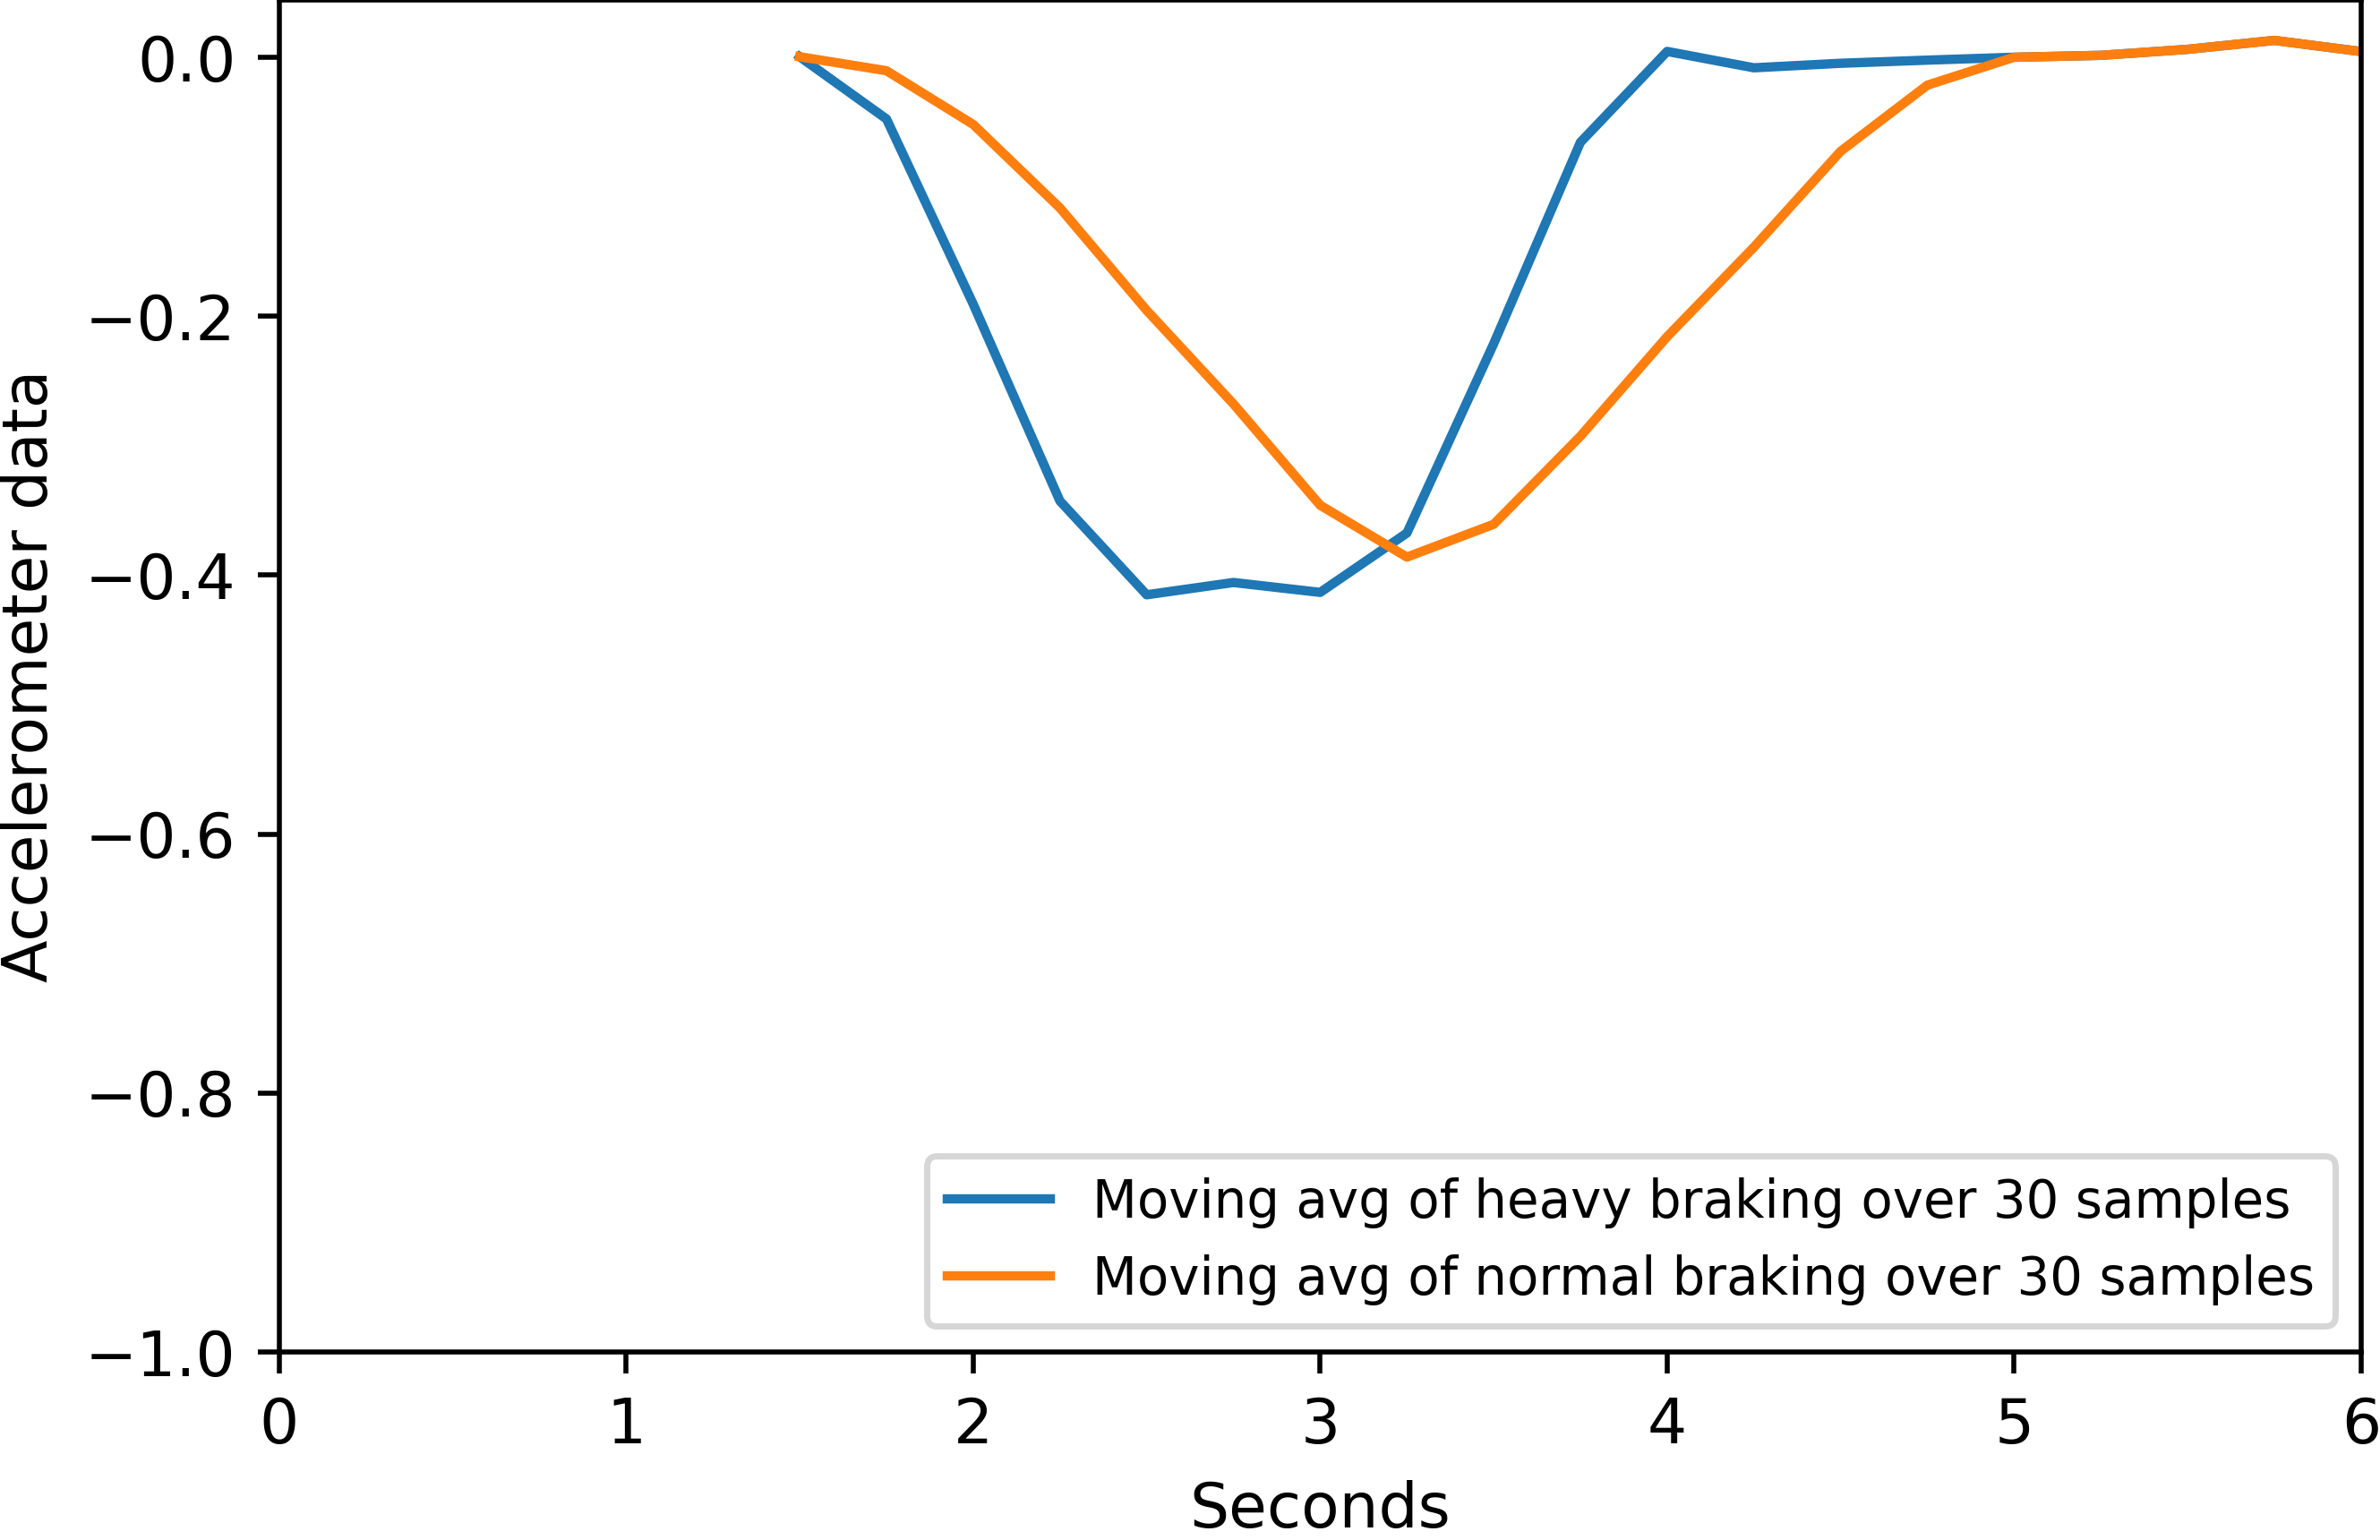
\includegraphics[width=\textwidth]{fig/mvn_avg_heavy_vs_normal_braking.png}
		%\caption{\small Moving average applied on the scaled accelerometer data of the original signal of an artificially modeled incident with heavy braking vs.\ an artificially modeled moderate braking event.}
	\end{subfigure}	
	\caption{Visualization of the sensor data of a simulated heavy braking incident vs.\ a moderate braking event before and after the moving average has been applied.}
	\label{fig:heavy-vs-normal-braking}
\end{figure}

\subsection{Limitation of the Classification Task}
\label{subsec:limitation_of_the_classification_task}
There is an inherent label imbalance present in our data set.
Only relatively few rides contain incidents. 
Moreover, the ratio between timestamps that represent an incident and those that do not is even smaller. 
As a consequence, there is an enormous imbalance between the different label categories.

Furthermore, some incident types such as tailgating or close passes might not be detectable at all in accelerometer and gyroscope sensors~\cite{aldred2018predictors, karakaya2020simra} as cyclists might not change their motion profile despite (or even due to) a dangerous situation.
For detecting these kinds of incidents it may be necessary to include different sensors.
In the SimRa project, this is already happening through an integration of \ac{obs}\footnote{https://www.openbikesensor.org/} data which measures the passing distance of cars.
The current data set, however, only includes very few OBS-supported rides.

In contrast to our classification task, the inherent classification problem of the \ac{har} data set \cite{anguita2013public}, is to classify reoccurring ongoing patterns such as walking or jogging, while an incident might need to be detected by one short non-reoccurring event such as sudden braking.
This further complicates the matter.

\subsection{Data Set Shift}
\label{subsec:data_set_shift}
A major challenge in the context of crowdsourced data are data set shifts. Depending on the device (see also \autoref{subsec:technical_limitations}), but also on other factors, such as the city of origin of the recorded data (see also \autoref{subsec:eval-results}), there could be non-stationarities in the data that violate the assumptions underlying almost all ML models and thus could impact the generalization performance of the trained models. Several types of data set shifts can be distinguished, including \textit{covariate shifts}, meaning shifts in the input data \cite{sugiyama_machine_2012}, \textit{label shifts}, meaning shifts in the distribution of targets \cite{lipton_detecting_2018}, or mixtures thereof. Detecting these shifts \cite{polyzotis_data_2018, rabanser_failing_2018, breck_data_2019, abdar_review_2021, bates_testing_2021} and predicting \cite{schelter_learning_2020} or reducing their impact on the generalization performance is an active field of research \cite{schelter_challenges_2018, biessmann_automated_2021}. Some approaches aim at model specific improvements to alleviate data set shift \cite{sugiyama_machine_2012}. These approaches have a decisive disadvantage, most of these approaches only work for one model class and require access to the inner workings of the ML pipeline, often after the feature extraction step. More promising and easier to build and maintain are model agnostic solutions that focus on the data, rather than the models, to detect and counteract data set shifts \cite{biessmann_automated_2021}. Extending the training data sets to account for all variation and shifts in the data that the ML model should be invariant to, often called \textit{augmentation}, is a popular and effective way of counteracting data set shift, see for instance \cite{cubuk_autoaugment_2019}. In our work we follow this line of thought of a data centric AI approach. 


\section{Alternative Approaches}
\label{sec:related_work_cyclesense}
One of the most common tasks for \ac{tsc} are Natural Language Processing, speech recognition, and audio recognition in general.
Another field that deals with this problem is \acf{har} which is concerned with identifying the specific activity of a human based on sensory time series data.
Time windows of a few seconds are classified into activity categories (e.g., walking, sitting, running, lying).
While various feature extraction and pattern recognition methods have been successfully applied in the past in this context~\cite{bulling2014tutorial}, those approaches have constraints such as hand-crafted feature extraction, being able to only learn shallow features~\cite{yang2015deep}, or the requirement for large amounts of well-labeled data for model training~\cite{wang2019deep}.
\acl{dl} techniques and more specifically \acp{cnn} have recently proven to overcome these issues and deliver convincing results in the context of \ac{har}~\cite{wang2019deep,ronao2015deep}.
Also, implementations of \acp{rnn} such as \ac{lstm}~\cite{tao2016multicolumn,yao2017deepsense} have proven to be successful.
Yao et al.\ \cite{yao2017deepsense} use a combination of \acp{rnn} and \acp{cnn} on top of a \ac{sf} approach after preprocessing their input data using a \ac{dft}.

\section{Summary}
\label{sec:summary_cyclesense}
An increased modal share of bicycles is necessary for solving emission and traffic related urban problems.
A key challenge for this, is the lack of (perceived) safety for cyclists.
Improving the situation requires detailed insights into safety levels of street segments -- the SimRa platform~\cite{karakaya2020simra} has been proposed as a data gathering mechanism for incidents and cycling tracks.
While this is an important step towards data collection, the platform relies on manual annotation of tracks which limits the number of potential users.

In this paper, we have proposed CycleSense -- a model for automatic detection of such incidents.
Using the SimRa data set, we have shown that CycleSense is capable of detecting incidents on the basis of accelerometer and gyroscope time series data in a real-world scenario.
It can correctly distinguish between an incident and a non-incident with a probability of up to 90.5\%.
We have also compared it to the heuristic currently used in the SimRa platform and an existing \ac{fcn} that was specifically developed for SimRa.
Additionally, we have implemented several \ac{dl} models that are frequently used in the context of \ac{tsc}.
We were able to show that our model outperforms all of these approaches.

While this is an important step towards fully automatic incident detection, we believe that -- in the context of the SimRa platform -- CycleSense should be complemented with human annotation in a semi-automated way for the foreseeable future.
Although this does not quite reach our long-term goal of full automation, it should significantly decrease the annotation effort and should also lead to improved labeling quality.
In the future, this could, in turn, be used to further improve CycleSense.
Since April 2022, the SimRa app has been using CycleSense for incident detection.




\chapter{Deriving Road Surface Quality from Bicycle Ride Data}
\label{cha:cyclequality}
In this chapter we present an approach for deriving the surface quality (or rather the lack of), which can be measured as vibrations or bumps, using the \ac{imu} built in smartphones.
In a second step, we can then combine data from multiple rides to derive an estimate for the surface quality.
This way, monitoring of surface quality can be automated to a high degree at little cost and the resulting data can be used for maintenance planning or surface quality-aware routing.
Especially for highly frequented cycling tracks, surface quality problems can be detected quickly.

While there are other projects studying the surface quality of cycling infrastructure through crowdsourcing (e.g., Luedemann et al.~\cite{luedemann2022bikevibes}), our work is unique and novel because alternative approaches (i) either focus on categorizing the surface \emph{type} (e.g., cobblestones) where we focus on the surface \emph{quality} (i.e., the level of roughness) or (ii) have strict assumptions on phone positioning and other properties where we rely on a ``wisdom of the crowds'' strategy to filter out noise.
The latter is also an advantage because, unlike related approaches, which use a dedicated app for measuring the road surface quality, thus, potentially forcing cyclists to run multiple apps, our approach can easily be retrofitted to existing apps and can even be used to analyze already stored datasets.

This chapter contains material published in \cite{karakaya2023crowdsensing} with following contributions:
\begin{itemize}
	\item We present a data processing pipeline for deriving surface quality which combines signal processing with geographical clustering techniques in the form of edge-based preprocessing on the phone and cloud analytics.
	\item We describe how we integrate this data processing pipeline in the existing crowdsourcing project SimRa~\cite{karakaya2020simra}(see \cref{sec:simra}) which previously only focused on incidents.
	\item We describe how the resulting data can be used to increase the comfort of cyclists through surface quality-aware routing and how the data can be exposed to city administrations.
	\item We evaluate our approach by analyzing the SimRa dataset~\cite{dataset_simra_set1,dataset_simra_set2,dataset_simra_set3} and comparing it on-site conditions in eight streets with different surface quality.
	\item We discuss to which degree our approach can automate surface quality monitoring and how additional sensors could possibly help to improve data quality.
\end{itemize}

We outlined this chapter as follows:
In \cref{sec:surface_quality_background} we give background information about the measurement of road surface quality.
We then continue with \cref{sec:scenarios_and_constraints}, where we clarify the scenarios and constraints of our approach.
We explain our approach and how it is integrated in SimRa (see \cref{sec:simra}) in \cref{sec:data_processing_pipeline}.
After that we describe two ways in which the road surface quality information can be used in \cref{sec:using_road_surface_quality_information}.
We follow this up with an evaluation and discussion of our approach in \cref{sec:evaluation_cyclequality} and \cref{sec:evaluation_cyclequality} respectively.
We conclude this chapter in \cref{sec:summary_cyclequality} after giving an overview of alternative approaches in \cref{sec:related_work_cyclequality}.

\section{Road Surface Quality}
\label{sec:surface_quality_background}
Traffic departments frequently analyze the road surface quality to find out road segments that need to be repaired to increase the traffic safety.
There are mainly three types of methods used for, which we briefly introduce here.
\textit{Profilographs} are one of the oldest devices used to measure road surface quality.
They consist of a profiling wheel in the center and multiple support wheels held together by a rigid frame.
They measure the road quality by tracking the vertical movement of the profiling wheel.
The higher the vertical movement of that wheel, the worse the surface quality of the road.
This method of measuring surface quality is very slow, since the profilograph has to be pulled very slowly by another vehicle.
\textit{Scanner-based systems} are more sophisticated and rely either on accelerometers measuring the vibrations caused by driving on a specific surface, lasers scanning the surface in front or beneath the vehicle, cameras making photos later to be analyzed with the help of computer vision and photogrammetry, or a combination of the aforementioned methods.
This system provides the highest resolution and accuracy, however it is also the most costly and complex one.
More recently, \textit{smartphone-based systems} are gaining traction due to their cost-efficiency.
A smartphone is being attached inside the car and the vibrations caused by the road surface are recorded.
This is the least accurate system, since the measured vibrations are very indirect, due to car tires and suspension.

However, these systems are impractical for measuring bicycle road surface quality, because cars are not suited to drive on bicycle roads and these systems are too costly.
Hence, we propose a novel system using crowdsourced smartphone bicycle ride data.

\section{Scenarios and Constraints}
\label{sec:scenarios_and_constraints}
The idea to use smartphones and crowdsourcing for tracking surface quality is not new.
For this reason, we use this dedicated section to briefly discuss the specific goals of our work and the unique constraints of the scenarios we target.
We do this to clarify why existing approaches, which we discuss in the next section, cannot solve the problem we target.

\begin{figure}[t]
    %\vspace{-3em}
    \centering
    \subfloat[Smooth cobblestones]{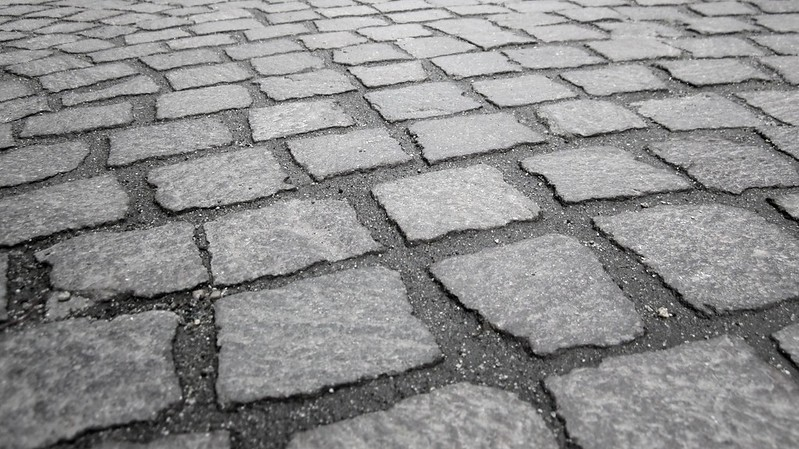
\includegraphics[width=0.4\columnwidth, height=4cm]{fig/cobblestone.jpg}}
    \hfill
    \subfloat[Rough asphalt]{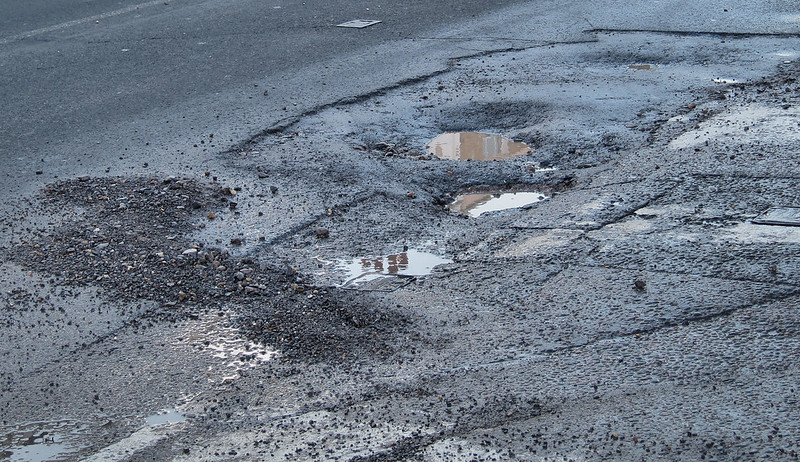
\includegraphics[width=0.4\columnwidth, height=4cm]{fig/asphalt.jpg}}
    \caption{%
        Smooth cobblestones can provide a good surface quality while bad asphalt can result in a bumpy ride (Source: Flickr.com).
    }%
    \label{fig:cobblestone_vs_asphalt}
\end{figure}

First, our work focuses on the experience in terms of ``bumpiness'' for cyclists.
Therefore, we try to quantify the roughness of a road surface and not its type.
As an example, a ride on asphalt will usually be smoother than one on a cobblestone road.
In practice, though, an asphalt road might have lots of (small) potholes and repair patches while a cobblestone road might use relatively flat (instead of rounded) stones  with mostly filled-in gaps between the stones.
See \cref{fig:cobblestone_vs_asphalt} for an example.
In such a setup, a ride on the cobblestone road can be much smoother.
Quantifying the surface \emph{quality} and not the surface \emph{type} will thus yield different results -- a large body of related work is hence not applicable to the problem we target.

Second, due to the width of bicycle tires, a single ride on a street segment will only cover a very small percentage of the surface.
Furthermore, cyclists are likely to swerve around the worst potholes and tree roots.
Both aspects combined show that it is crucial to base the roughness measurements on a large number of rides, thus, following a ``wisdom of the crowds'' approach.
We hence have to attract a large user group -- this has a number of implications.
\begin{enumerate}
	\item The approach needs to go easy on the phone's resources (battery, data transmission, compute power, app size) as users will otherwise uninstall or not use the corresponding app. As a result, the approach will have to prefilter data on the phone but is unlikely to run on the phone completely, machine learning-based approaches may be problematic, and the approach cannot expect high resolution raw data.
	\item The approach should not have physical setup requirements. Some cyclists mount their phones on the handlebar (which usually will yield the best results for using accelerometer sensors), others keep it in pockets, backpacks, etc. Any approach that \emph{requires} cyclists to use a certain setup will deter a large number of potential users. As an implication, many approaches that work under lab conditions will not work on the street.
	\item The approach needs to easily integrate into existing cycling apps. As we have seen in SimRa~\cite{karakaya2020simra}, many cyclists will not use more than one cycling app in parallel. To maximize the potential user base, the approach hence needs to be designed in a way that it can easily be integrated into existing cycling apps. In general, this means that the approach needs to run as an independent background job and may not involve manual labeling and similar activities. They may also be subject to privacy-related restrictions.
\end{enumerate}

The approach we present in this section was designed around these constraints.
We retrofitted it to the SimRa app~\cite{karakaya2020simra} but it could easily be integrated as a plugin in, e.g., Strava or BikeCitizens.
As a soft constraint, we tried (and succeeded) to design our approach in a way that it can also process our existing datasets~\cite{dataset_simra_set1,dataset_simra_set2,dataset_simra_set3}.


\section{Integrating Road Surface Quality Measurement into SimRa}
\label{sec:data_processing_pipeline}
In this section, we start by giving a high-level overview of our data processing pipeline for deriving surface quality (\cref{subsec:overview_of_pipeline}) before describing how we derive the surface quality (\cref{subsec:surface_quality_analysis}).


\subsection{Overview of Pipeline}
\label{subsec:overview_of_pipeline}
\begin{figure}
    \centering
    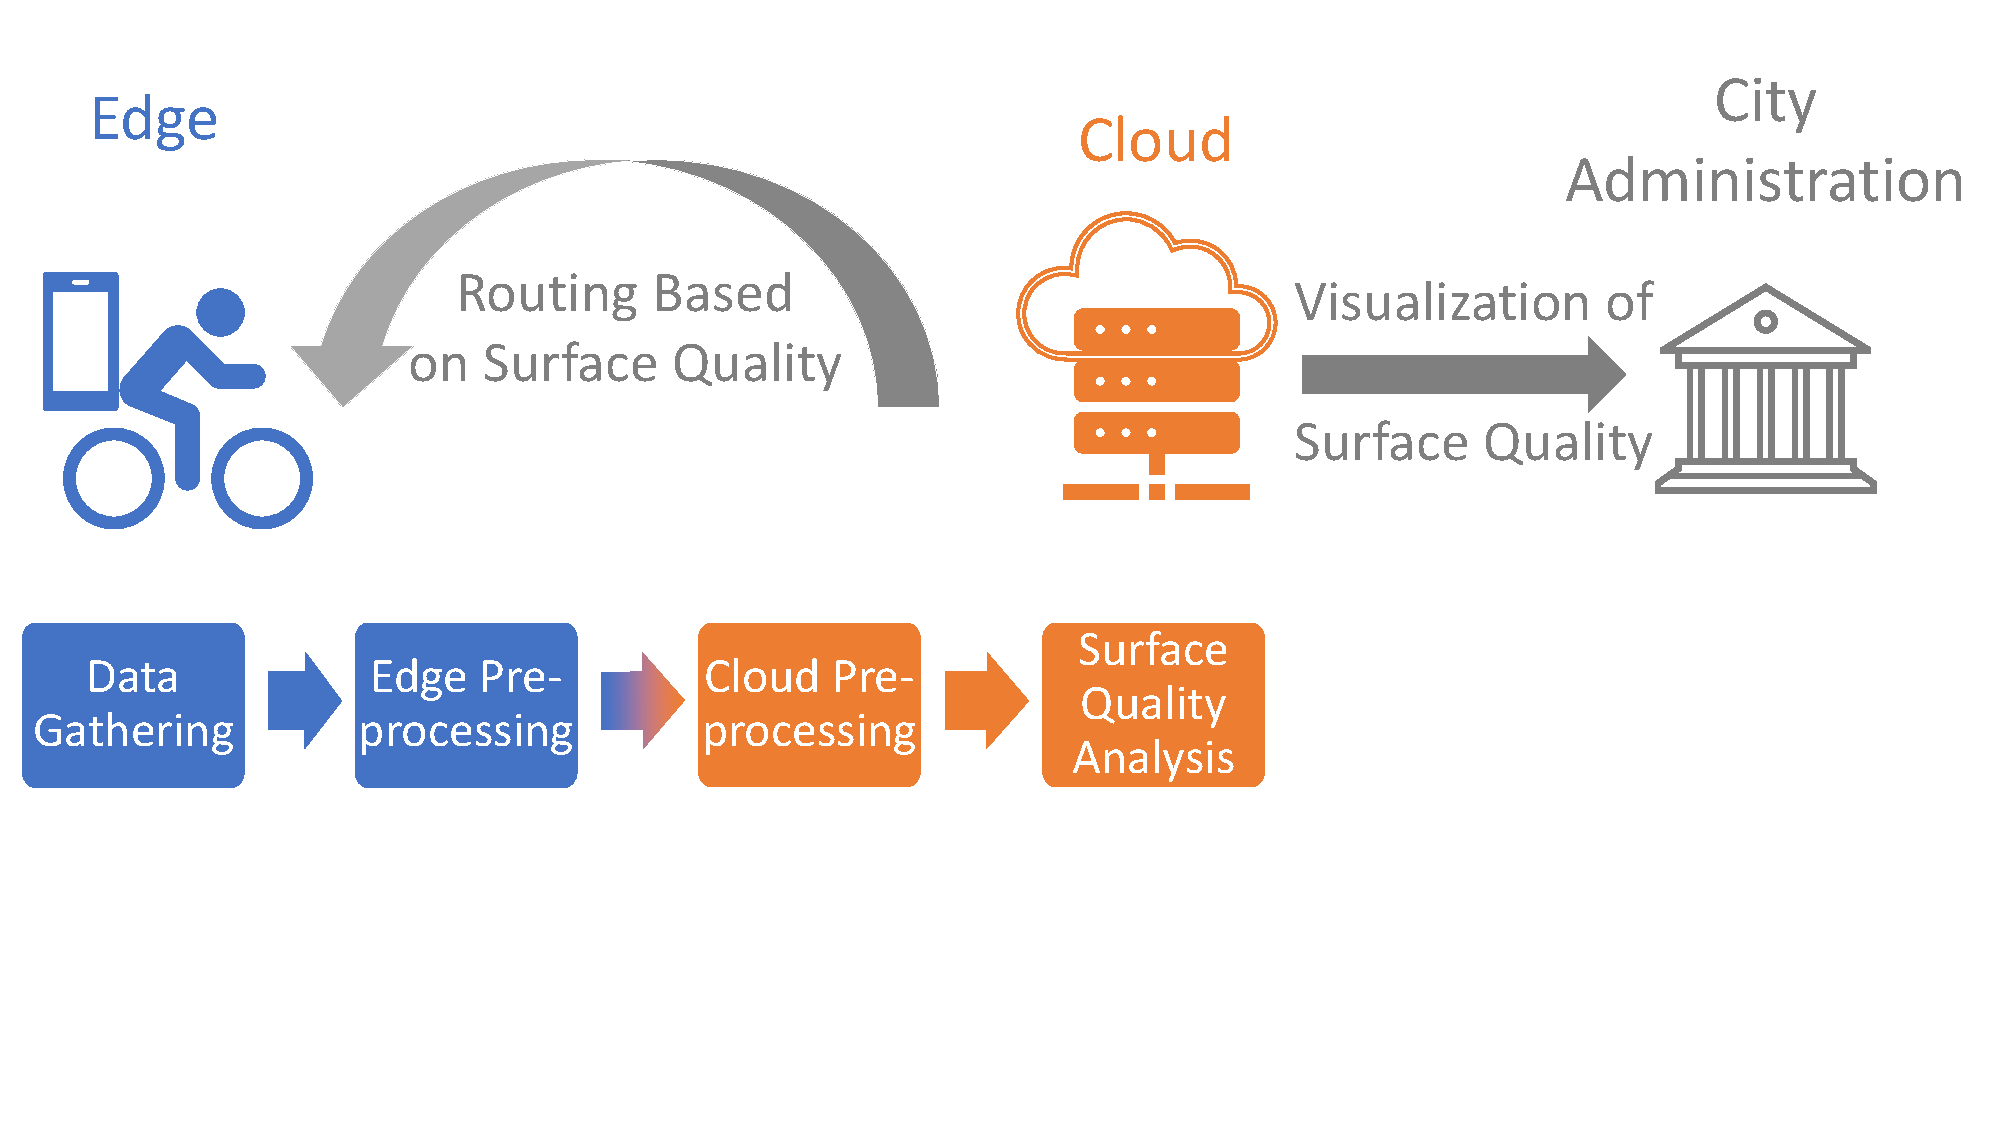
\includegraphics[width=\columnwidth]{fig/overview.pdf}
    \caption{%
        Overview of our surface quality analysis pipeline.
    }%
    \label{fig:overview}
\end{figure}
The tasks of our data processing pipelines are distributed over the edge (i.e., on the smartphone) and the cloud, see also \Cref{fig:overview}.
After collecting data in the SimRa app (see \cref{sec:simra} using the built-in motion sensors, data is preprocessed locally before upload to our backend servers.
There, additional preprocessing steps are executed before the actual surface quality analysis.

The parts of the preprocessing which reduce the amount of data need to be run on the edge to preserve user privacy and to reduce bandwidth consumption.
The data cleaning parts are too compute-intensive and are executed in the cloud to reduce power consumption on the phone.

\subsection{Surface Quality Analysis}
\label{subsec:surface_quality_analysis}
Each cyclist creates a different data track on a given road, and without calibration, it is not possible to accurately analyze each track individually.
Ideally, we would at least use cyclist-specific profiles (i.e., per cyclist aggregates) which, however, are not available due to privacy reasons (rides are pseudonymized individually~\cite{karakaya2020simra}).
The idea behind our approach is to take advantage of the size of the data set and use the law of large numbers to obtain robust results without having to calibrate the data and without affecting the results too much by noise.

For this, we consider in the first step each ride individually:
We take the preprocessed ride (which is a single time series of aggregated motion sensor readings without stops plus the GPS trace) and calculate the percentiles (0.2, 0.4, 0.6, 0.8, and 1) of the time series.
For normalization, we then replace all motion sensor readings with values 1 to 5 depending on which interval they fall into, i.e., a motion sensor reading from the interval $(0.2;0.4]$ would be replaced with the value 2.
The intuition behind this is that longer rides are likely to encounter very different surface quality, hence we calculate the relative bumpiness of an area in comparison to the rest of the ride's bumpiness.

In the second step, we use the data from all such normalized rides and, using the GPS trace, map them to a grid of 10m² cells.
For each cell, we hence have a distribution of values 1 to 5.
As a metric for the bumpiness of that cell, we use the average of all values -- e.g., when color-coding a map -- but make other statistical metrics available as well (see, e.g., the distribution function charts in our evaluation section).

\section{Using Road Surface Quality Information}
\label{sec:using_road_surface_quality_information}
In this section, we describe how such surface quality results can be used.
In \cref{subsec:routing_with_surface_quality}, we describe how we implement a navigation feature into the SimRa app that uses the road surface quality as an additional parameter in routing.
We then show in \cref{subsec:output_data_and_visualization} how we can expose the output data of our pipeline to city administrators.


\subsection{Routing with Surface Quality}
\label{subsec:routing_with_surface_quality}
With the surface quality scores calculated, it is possible to provide a route planning feature, where not only distance and time are considered, but also the surface quality.
The main question here is how much the surface quality should be weighed when calculating the best route from A to B or rather what detour lengths are acceptable.
We decided to give the user the opportunity to influence this factor with the usage of a slider, that can be set between 0 for not considering surface quality in the routing and 10 for the highest importance of the surface quality (\cref{fig:routing}).
 \begin{figure}
    \centering
    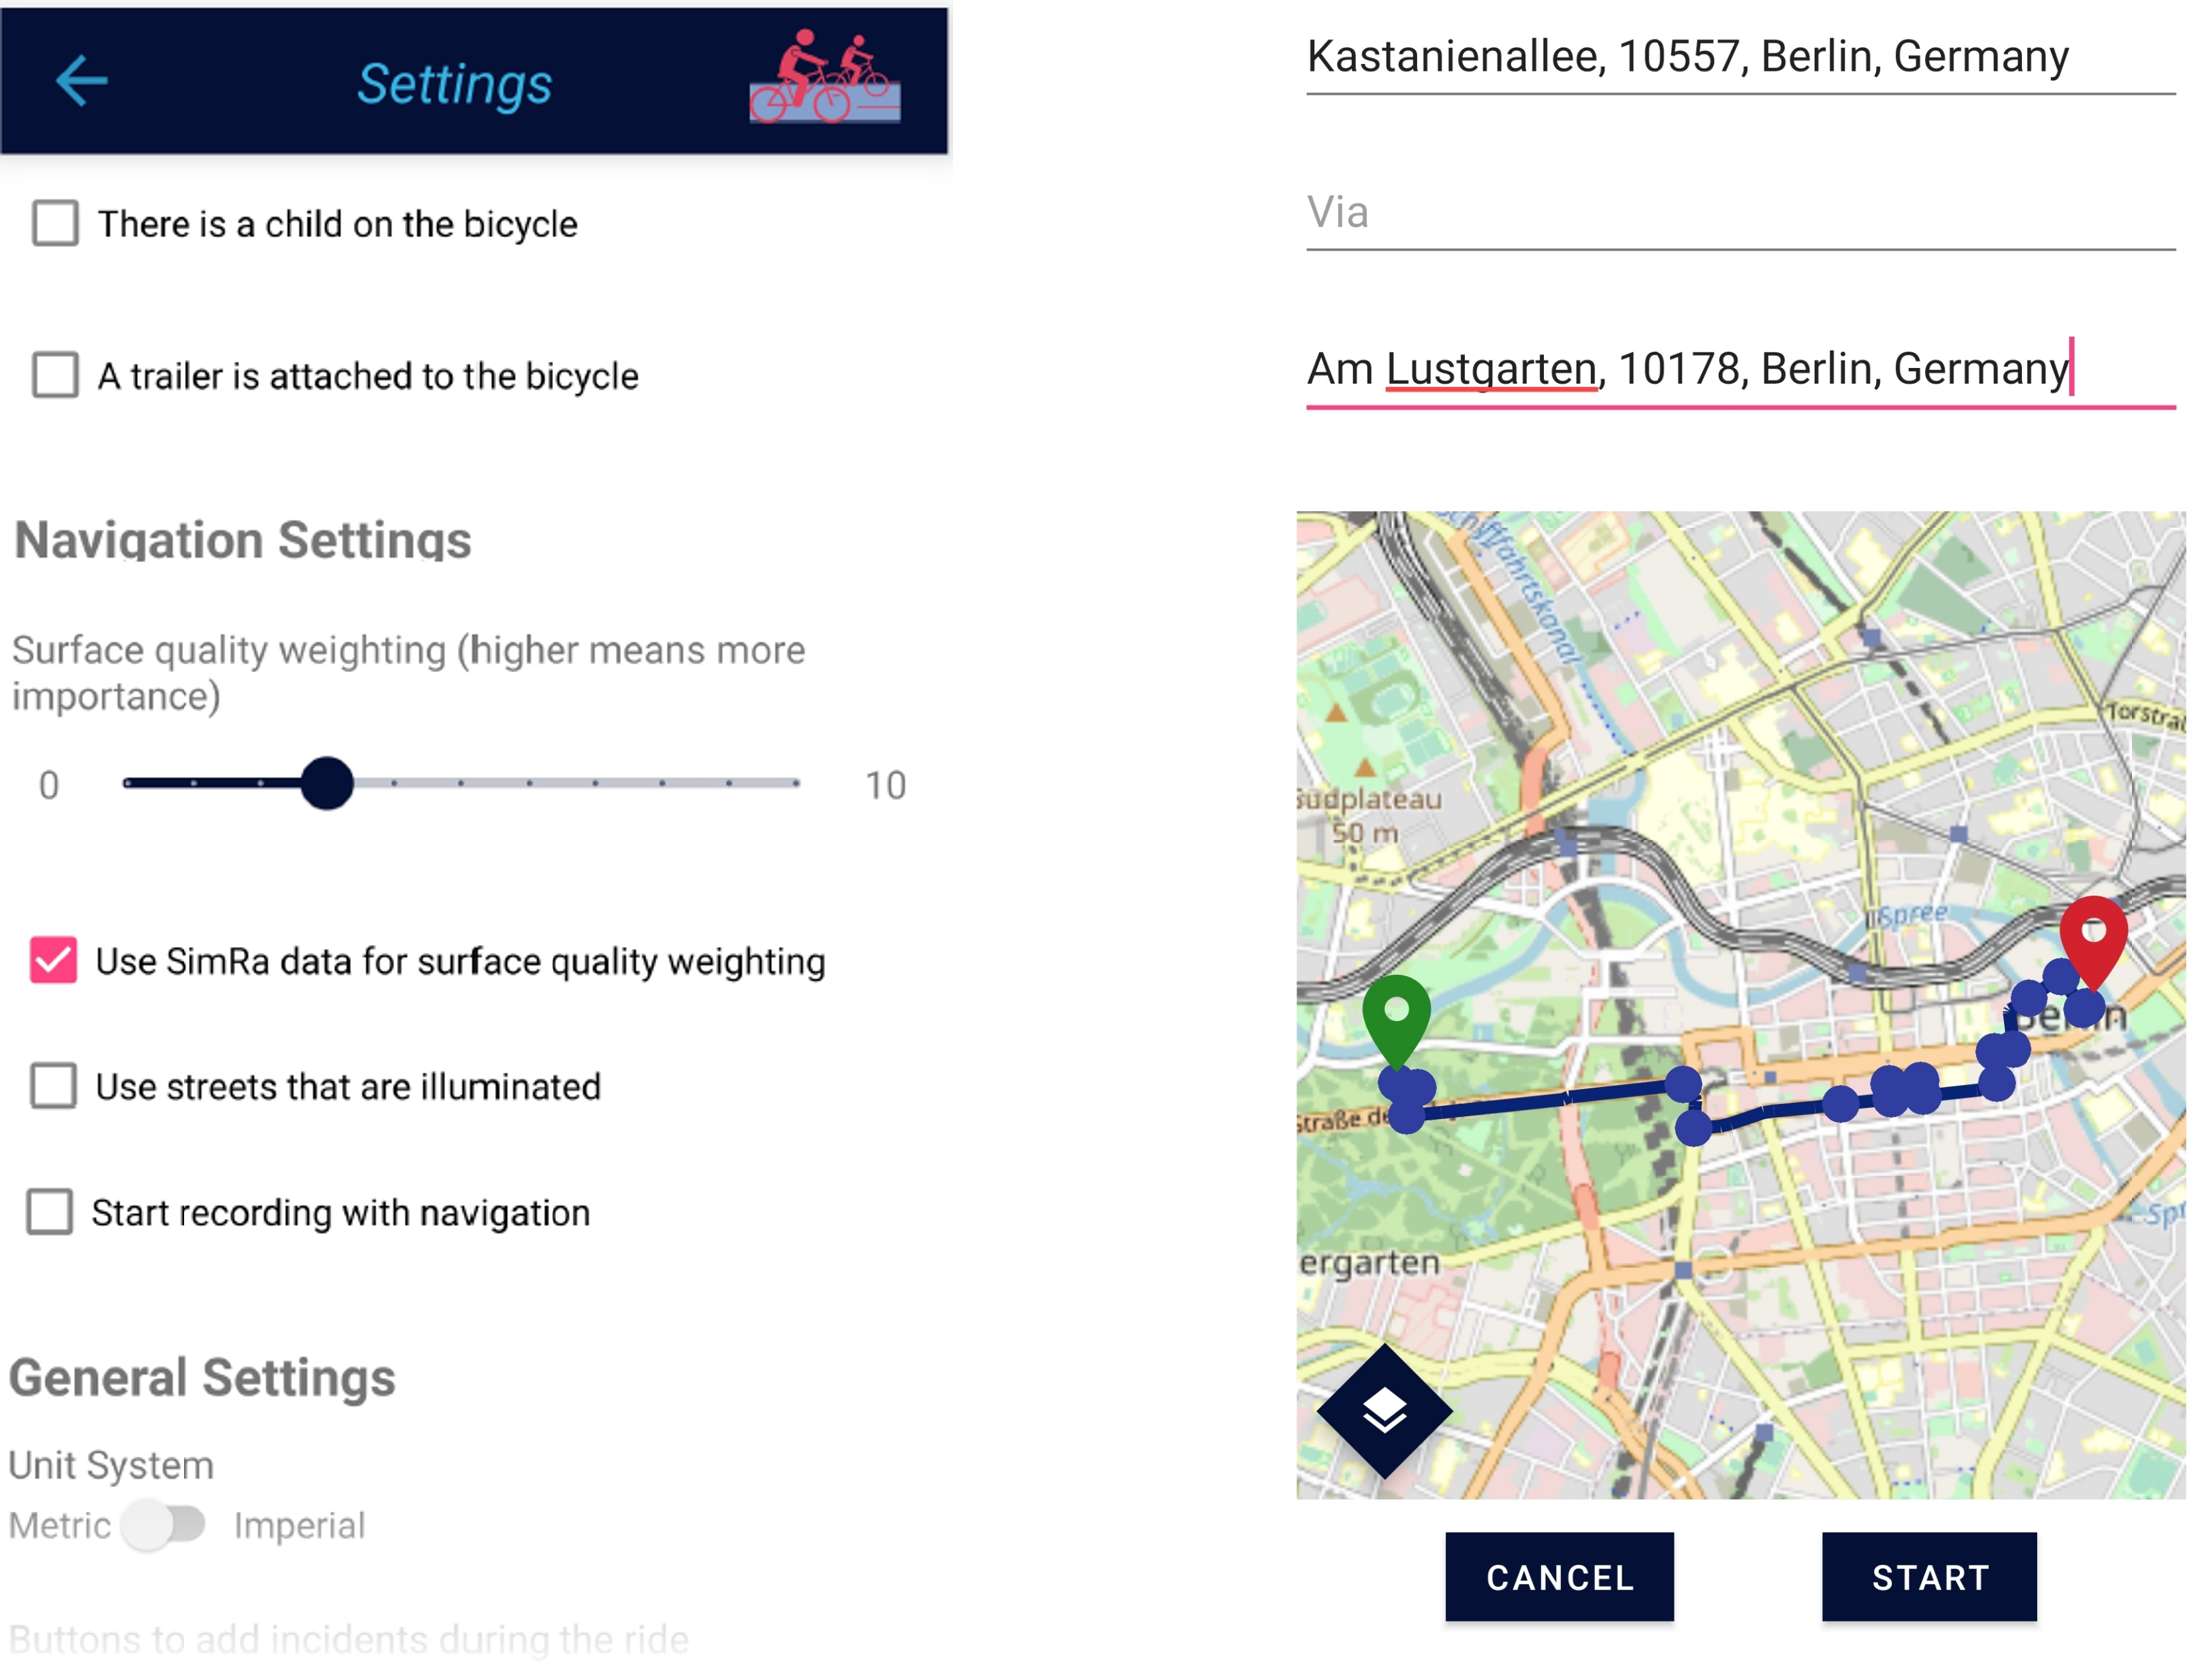
\includegraphics[width=0.7\columnwidth]{fig/routing_settings_2.png}
    \caption{%
With a slider in the settings menu, the weight of the surface quality in the routing can be set.}%
    \label{fig:routing}
\end{figure}
We host a modified GraphHopper\footnote{https://github.com/graphhopper/} for routing.
GraphHopper uses edges for streets, that are connected via nodes.
Each has a weight for routing purposes and it is possible to change the weight according to custom data.
This is where we use the surface quality by increasing the weight depending on surface quality and user-specified influence factor.

\subsection{Output Data and Visualization}
\label{subsec:output_data_and_visualization}
Our bicycle road surface quality pipeline creates a GeoJSON file as an output.
It contains the cells with a surface area of 10m² in a grid as \codeword{Features} of the \codeword{geometry} type \codeword{Polygon} with the surface quality score information such as mean, median, standard deviation, number of rides going through the cell and coloring information in the \codeword{properties} key.
 \begin{figure}
    \centering
    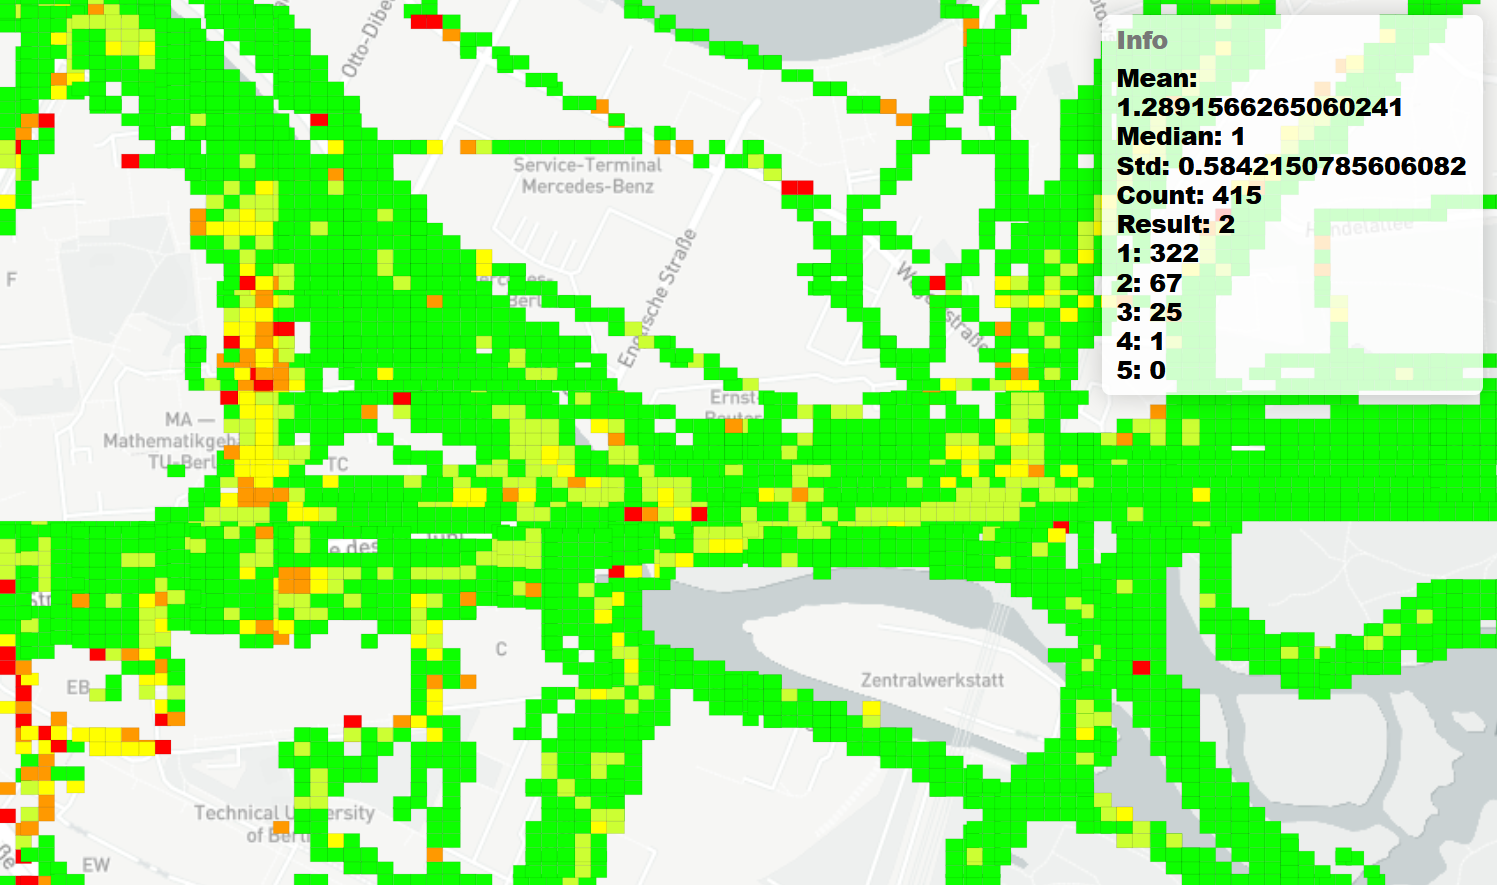
\includegraphics[width=0.7\columnwidth]{fig/visualization.png}
    \caption{%
A visualization of the output file showing the surface quality of the boxes when hovering over them with the mouse cursor. Color coding is based on the average value.}%
    \label{fig:visualization}
\end{figure}
With such an output file, it is very easy to create a simple visualization\footnote{https://simra-project.github.io/surfaceQuality/Berlin.html}, e.g., with Leaflet\footnote{https://leafletjs.com/}, as depicted in \cref{fig:visualization}.
Using a visualization like this, also non-tech-savvy users can easily monitor the bicycle road surface quality of a large area and take action where needed.


\section{Evaluation}
\label{sec:evaluation_cyclequality}
In this section, we evaluate the surface quality analysis by comparing the calculated surface quality of selected street segments across Berlin with their surface type in the real world, which we get from OpenStreetMap (OSM).
As data input, we use the existing SimRa datasets~\cite{dataset_simra_set1,dataset_simra_set2,dataset_simra_set3} (almost 90,000 rides with more than 650,000km in total\footnote{All numbers in this chapter regarding the SimRa dataset are as of September 2022}).
Based on the intuition that different surface types will also be partially correlated with surface quality, we randomly picked four spots with different surface types.
To also show the limitations of our approach, we then explored the dataset and manually picked four additional spots where our approach appears to have returned the wrong results.
Each evaluated section has a surface area of 10 m² and to compare them to each other we analyze their mean, median, and standard deviation values.

We first describe the clear results from the first group (\cref{subsec:sections_with_clear_results}).
Afterwards, we categorize the additional four ``problem spots'' as mixed results (\cref{subsec:sections_with_mixed_results}) or seemingly incorrect results (\cref{subsec:sections_with_seemingly_confusing_results}).


\subsection{Sections with Clear Results}
\label{subsec:sections_with_clear_results}
We evaluate at least one example for each of the following surface types, which are sorted in descending order with regard to their expected surface quality~\cite{titov2019monitoring}: asphalt, flat paving stones, fine gravel, cobblestones.
We chose the sections in a way that (i) asserted that we have sufficient data for them and (ii) to cover all different surface types.
After filtering based on these criteria, we randomly picked four sections.

\cref{tab:clear} and \cref{fig:clear} show the results of the surface quality analysis of the selected sections with very clear and intuitive results.

\begin{figure}
    \centering
    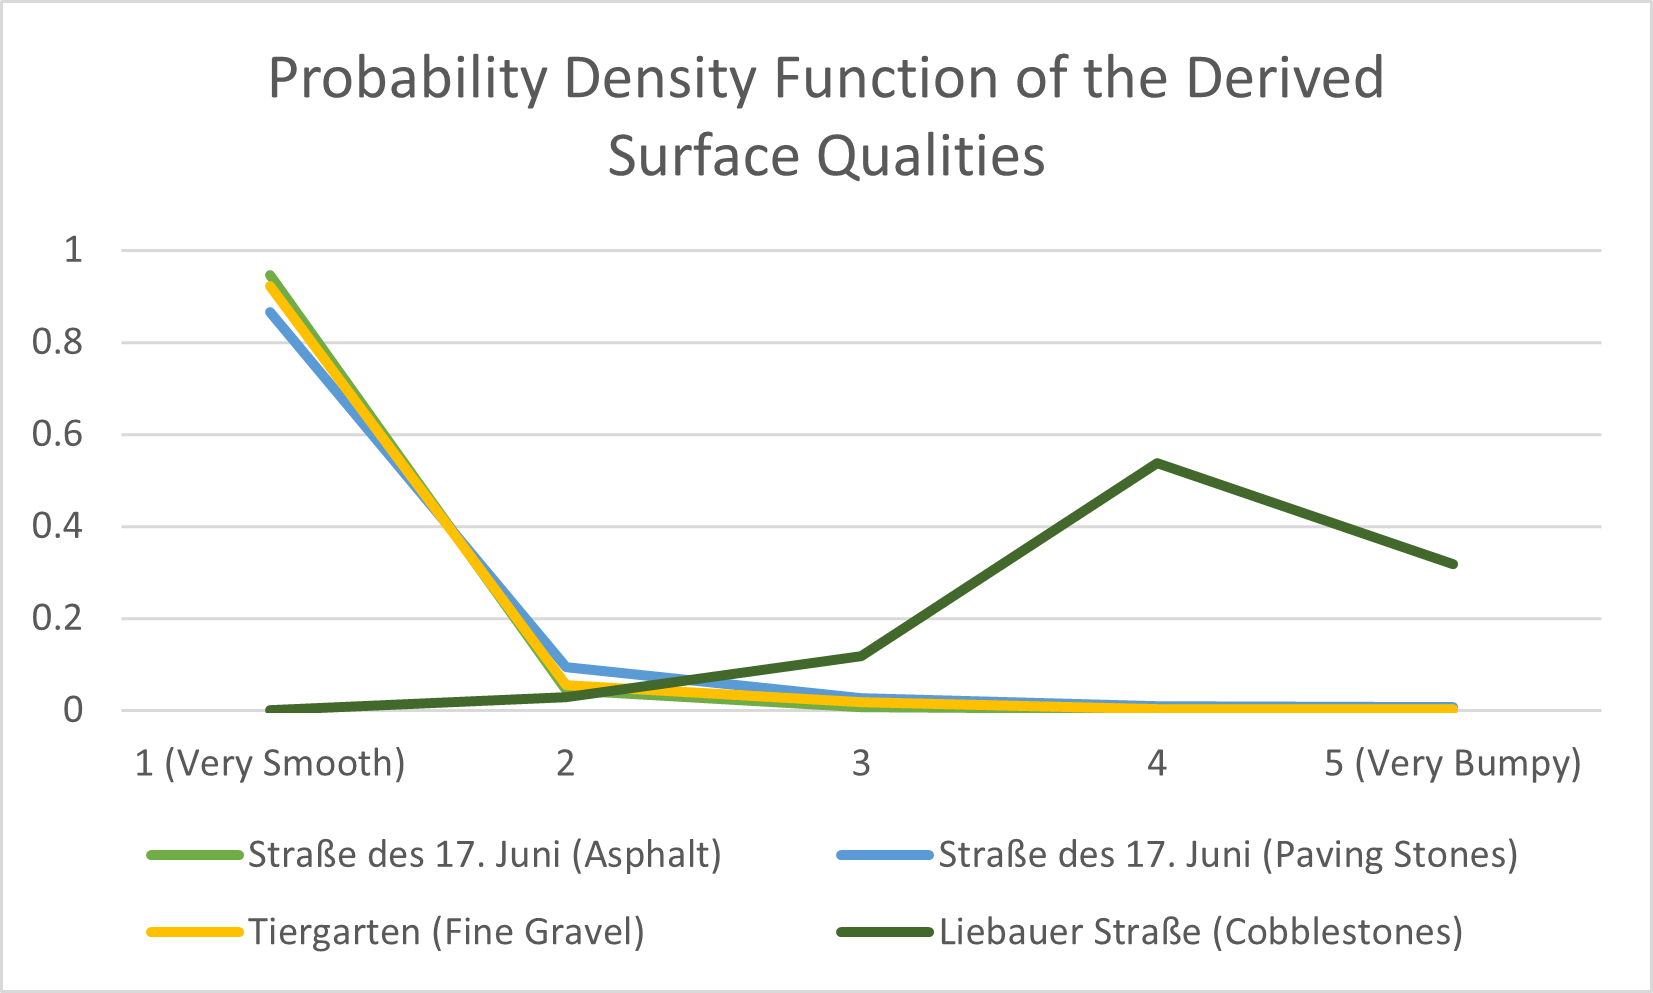
\includegraphics[width=0.7\columnwidth]{fig/pdf_clear.png}
    \caption{%
        The Probability Density Function of the Derived Surface Qualities shows that these segments have very undisputed road surface quality values, since they are either very good or very bad.
    }%
    \label{fig:clear}
\end{figure}

It can be observed, that the aforementioned list of surface types, which was sorted in descending surface quality order, was ordered correctly.
A newly maintained asphalt section in \textit{Straße des 17. Juni} has a nearly perfect score, which means that its surface quality was in the top 20\% in almost all rides crossing this section.
Followed by that are two sections with flat paving stones and fine gravel as their surface type, which have very similar results.
This means, that both flat paving stones and fine gravel have comparable surface quality in terms of bumpiness from the perspective of a cyclist.
However, it should be noted, that fine gravel can be less favorable in areas with a lot of precipitation (more on that in \cref{sec:discussion_cyclequality}).
Not very surprisingly, the \textit{Liebauer Straße} has very bad surface quality scores, since it is paved with cobblestones and has very busy sidewalks with restaurants and cafes, which prevent cyclists from (illegaly) cycling there instead of on the street.

\begin{table}%
\centering
\caption{Surface Quality Analysis Evaluation Results Showing Mean, Median and Standard Deviation of Sections With Clear Results}%
\label{tab:clear}
\resizebox{\columnwidth}{!}{
\begin{tabular}{cccccc}%
\toprule%
Street Name          & Surface       & GPS Location        & Mean & Median & Std. Dev.\\%
\midrule%
\midrule%
Straße des 17. Juni  & Asphalt       & 52.515369,13.630855 & 1.03 & 1      & 0.17\\%
Straße des 17. Juni  & Paving Stones & 52.513501,13.335127 & 1.25 & 1      & 0.5\\%
Tiergarten           & Fine Gravel   & 52.514745,13.34622 & 1.32 & 1      & 1.06\\%
Liebauer Straße      & Cobblestones  & 52.509132,13.453806 & 4.15 & 4      & 1.07\\%
\bottomrule&%
\end{tabular}%
}
\end{table}

\subsection{Sections with Mixed Results}
\label{subsec:sections_with_mixed_results}
While most results are intuitive, e.g., new bicycle roads paved with asphalt and separated from the motorized vehicle traffic having very good surface conditions, some other sections (see \cref{fig:mixed}) seem confusing at the first glance.

\begin{figure}
    \centering
    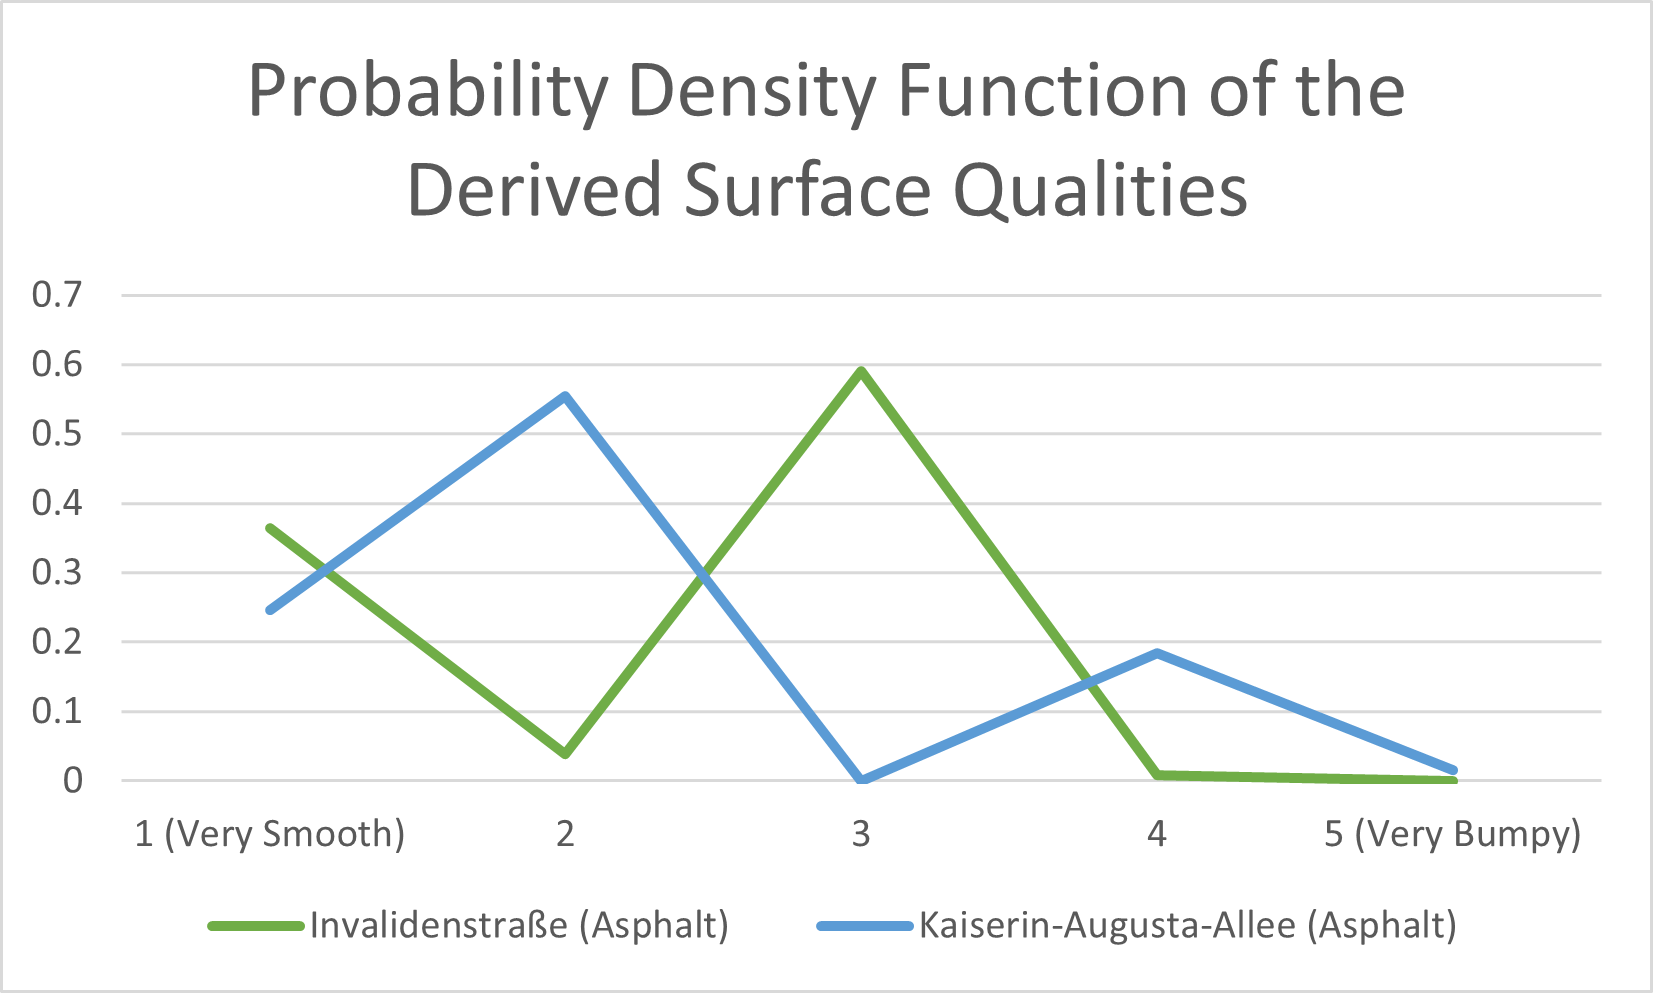
\includegraphics[width=0.7\columnwidth]{fig/pdf_mixed.png}
    \caption{%
        The Probability Density Function of the Derived Surface Qualities shows that these segments have confusing road surface quality values: Depending on the ride, they appear to have either very good or very bad surface quality (multiple peaks).
    }%
    \label{fig:mixed}
\end{figure}

According to the Probability Density Functions (PDFs) of street sections in the \textit{Invalidenstraße} and \textit{Kaiserin-Augusta-Allee}, there seem to be two distinct surface qualities in each section.
A closer look into the specific sections reveal the causes:
 
\begin{table}%
\centering
\caption{Surface Quality Analysis Evaluation Results Showing Mean, Median and Standard Deviation of Sections With Mixed Results}%
\label{tab:mixed}
\resizebox{\columnwidth}{!}{
\begin{tabular}{cccccc}%
\toprule%
Street Name          & Surface       & GPS Location        & Mean & Median & Std. Dev.\\%
\midrule%
\midrule%
Invalidenstraße           & Asphalt   & 52.526236,13.369196 & 2.24 & 3      & 0.96\\%
Kaiserin-Augusta-Allee      & Asphalt  & 52.524429,13.327253 & 2.17 & 2      & 1.05\\%
\bottomrule&%
\end{tabular}%
}
\end{table}

In \textit{Invalidenstraße}, there are a bus lane, a bus stop, and an on-curb bike lane (see \cref{fig:invaliden}).
Most bus lanes in Berlin can be legally used by cyclists, however, some cyclist may still prefer the relatively bumpy bike lane.
\begin{figure}
    \centering
    \includegraphics[width=0.7\columnwidth]{fig/invalidenstr.png}
    \caption{%
        A bus lane, a bus station and a bicycle lane on the sidewalk can create different results in a small area. (Source: Apple Maps)
    }%
    \label{fig:invaliden}
\end{figure}
Additionally, when a bus stops at the bus station, cyclists that used the bus lane might overtake the bus on the very smooth car lane to the left. 
These two factors most certainly are the reason for the distinct two-peak distribution of recordings in that spot.

A closer look at the near-miss incident data in \textit{Kaiserin-Augusta-Allee} indicates that people use the bike lane in one direction and the street in the other direction~\cite{dataset_simra_set1,dataset_simra_set2,dataset_simra_set3} as one side seems to be in an unusable condition while the other is acceptable.
Since the bicycle lane is paved with paving stones and the street with asphalt, this leads to different surface quality of the road, depending on which direction the ride was.
Both directions, however, regularly end up in the same 10x10m box as the street is not overly wide, especially considering GPS accuracy.

\subsection{Sections with (Seemingly) Confusing Results}
\label{subsec:sections_with_seemingly_confusing_results}
There are also sections where the surface quality result seem to be completely wrong, when compared to the OSM surface type labels.
\Cref{tab:mismatch} shows two sections, that are -- according to OSM -- paved with cobblestones and without separate bike lanes, but with very good results, which is confirmed by the PDFs depicted in \cref{fig:mismatched}.

\begin{figure}
    \centering
    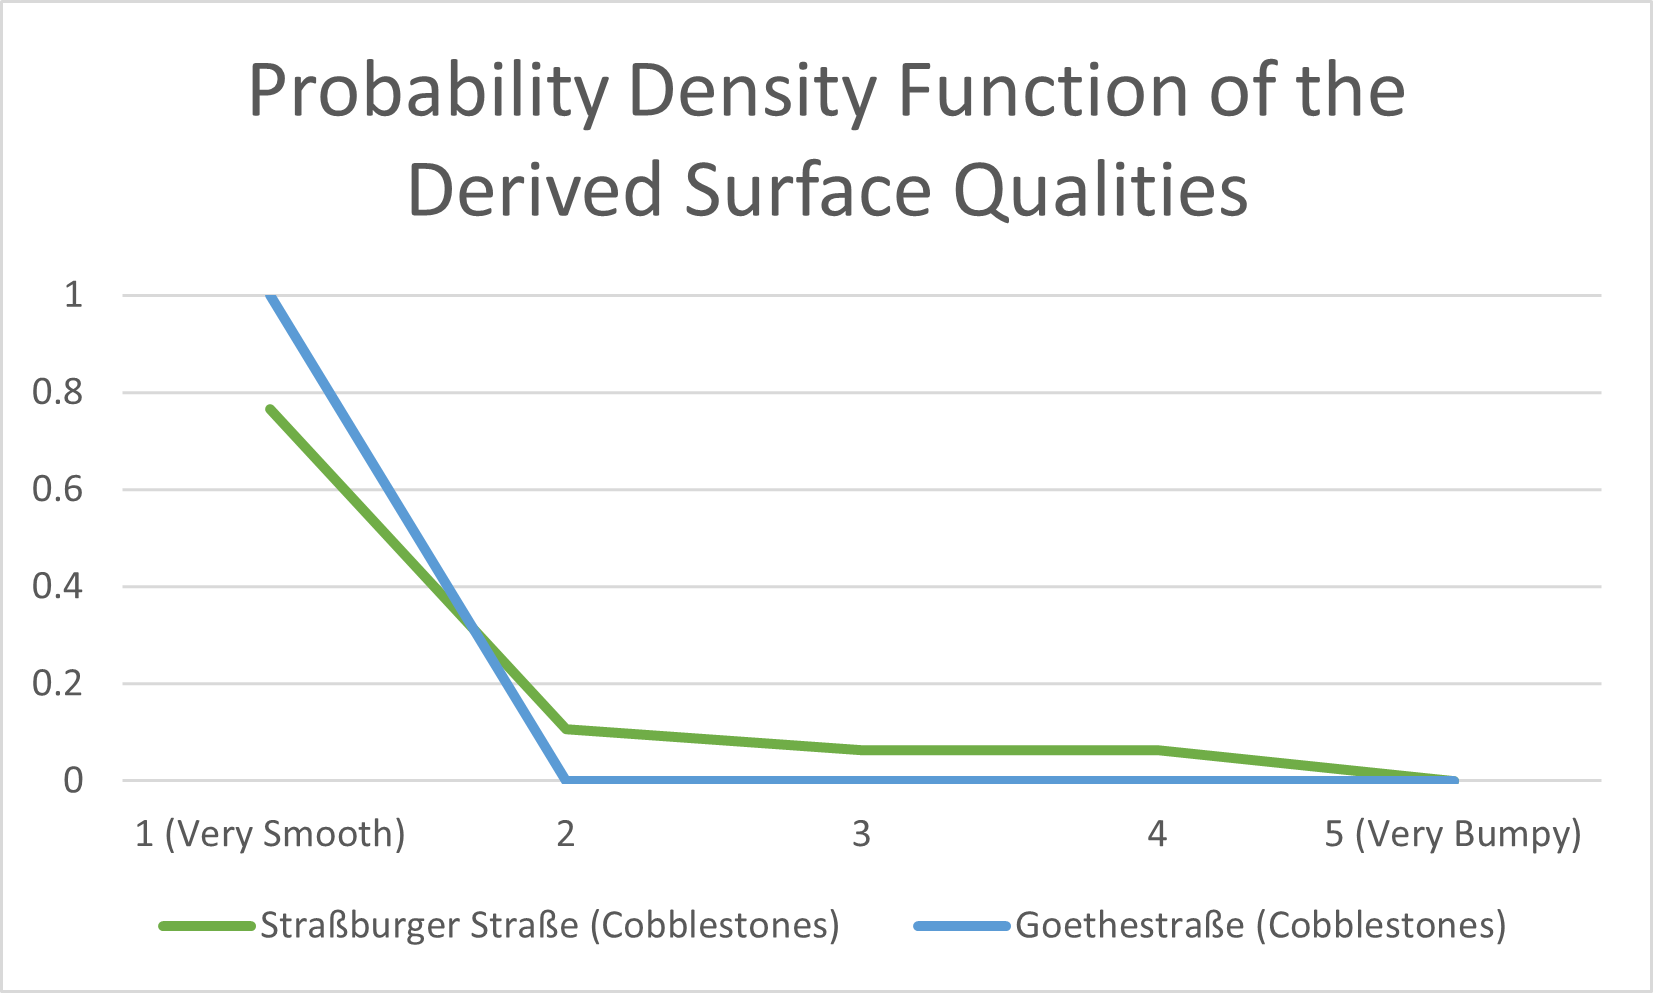
\includegraphics[width=0.7\columnwidth]{fig/pdf_mismatched.png}
    \caption{%
        The Probability Density Function of the Derived Surface Qualities shows that these segments have very smooth road surfaces, although they are paved with cobblestones.
    }%
    \label{fig:mismatched}
\end{figure}

The possibility, that this section has a wrong label and is in fact, not paved with cobblestones may come to mind.
However, as \cref{fig:sidewalk} reveals, both streets are indeed paved with cobblestones.

\begin{figure*}[t]
    %\vspace{-3em}
    \centering
    \subfloat[Straßburger Straße]{\includegraphics[width=0.4\columnwidth]{fig/straßburger_str_2.png}}
    \hfill
    \subfloat[Goethestraße]{\includegraphics[width=0.4\columnwidth]{fig/goethestr22.png}}
    \caption{%
        Straßburger Straße and Goethestraße in Berlin are paved with large cobblestones and the roads are contested by cars that are parking or searching for a parking spot. In contrast, the sidewalks are paved with flat-surfaced paving stones and are quiet due to the absence of shops, restaurants or cafes. (Source: Apple Maps)
    }%
    \label{fig:sidewalk}
    \vspace{-.5em}
\end{figure*}

\Cref{fig:sidewalk} also shows very likely reasons why these sections have very smooth bicycle rides.
The infrastructural conditions incentivize cyclists to prefer the sidewalks over the actual streets.
First, the cobblestones on the streets make it very unpleasant for cyclists to cycle on them.
Second, the sidewalks are wide, quiet, and paved with large flat-surfaced paving stones.
Third, the streets are contested by parking cars, or by cars searching for a parking spot, service vehicles, construction vehicles, etc. which will often block cyclists and also create safety hazards.
Considering these circumstances, it is not surprising to see good surface quality values in these two and other similar streets as cyclists are likely to (illegaly) use the sidewalks instead.
In fact, photos on Apple Maps (not included in this paper) actually show cyclists using the sidewalk instead.

\begin{table}%
\centering
\caption{Surface Quality Analysis Evaluation Results Showing Mean, Median and Standard Deviation of Sections With (Seemingly) Confusing Results}%
\label{tab:mismatch}
\resizebox{\columnwidth}{!}{
\begin{tabular}{cccccc}%
\toprule%
Street Name        & Surface     & GPS Location        & Mean & Median & Std. Dev.\\%
\midrule%
\midrule%
Straßburger Straße & Cobblestone & 52.532273,13.416521 & 1.43 & 1      & 0.87\\%
Goethestraße       & Cobblestone & 52.508889,13.308333 & 1    & 1      & 0\\%
\bottomrule&%
\end{tabular}%
}
\end{table}

\section{Discussion}
\label{sec:discussion_cyclequality}
Overall, the results presented in this paper show, that our approach can derive surface quality information using data recorded in the SimRa app.
Nevertheless, it still has a number of limitations which we discuss in this section.
Note that we also discuss some limitations in \cref{cha:discussion_and_outlook}, that may also apply to this approach.


\subsection{Behavior of Cyclists}
\label{subsec:behavior_of_cyclists}
Due to the GPS inaccuracy, it is impossible to identify whether a cyclist used the actual road or the sidewalk.
For instance, as discussed in the previous section, \cref{fig:sidewalk} showing \textit{Straßburger Straße} in Berlin, would be expected to have poor results but in fact has surprisingly good values.
We believe that this is due to cyclists illegaly using the smooth sidewalk instead of the bumpy road.

Furthermore, cyclists will in practice also avoid the worst potholes and similar bumps if possible, i.e., these will usually be missing from our analysis.

\subsection{Sensor Inaccuracy}
\label{subsec:sensor_inaccuracy}
The inaccuracy of the GPS sensors~\cite{merry2019smartphone} combined with noise produced by the motion sensors of the smartphones form another limitation of the dataset.
We tried to partially address these limitations with our preprocessing steps but they can, of course, not be fully mitigated.
The only alternative would be using dedicated hardware which, however, will result in significantly less recorded rides due to the adoption barrier.

\subsection{Temporal Influences}
\label{subsec:temporal_influences}
The rides in the SimRa dataset date back up to 2019 and it is possible that the surface quality changed throughout the time.
One reason for that could be that the surface type is changed for example from cobblestones to asphalt or potholes and cracks are repaired.
This would presumably lead to better results after the change, but show up as two-peak distribution in our dataset.
When using this approach in practice, we hence propose to only consider the most recent rides.

Another temporal influence might be the weather.
On rainy, windy or snowy days, the surface quality of the road, especially with wet gravel, can suffer significantly, which is not considered by our surface quality analysis approach.
However, adding this factor to the analysis, would in our dataset reduce the validity of the results, since it would reduce the number of considered rides.


\section{Alternative Approaches}
\label{sec:related_work_cyclequality}
Surface quality is usually quantified based on the International Roughness Index (IRI), e.g.,~\cite{sayers1986The}.
Traditionally, this was done using so-called profilographs (approximately resembling a large ladder with wheels) which are towed by a car or pushed manually.
A study from the 1980s~\cite{cumbaa1986road} found that they often break down and are difficult to maneuver in narrow streets which renders them infeasible for measuring the quality of bike lanes.
Furthermore, such measurement are very personnel-intensive which makes it unrealistic to apply them on a broad scale.

Taniguchi et al.~\cite{taniguchi2015evaluation} detect road hazards such as debris, potholes, or bumps.
For this, they attach an ultrasonic distance sensor to a bike handlebar, scanning the ground in front of the bicycle.
While the approach can warn cyclists about incoming bumps on the road ahead in real-time, this approach does not scale for city-wide analysis due to the sheer number of sensors needed.

Peng et al.~\cite{peng2019road} follow the same goal, using motion sensors instead of distance measurements.
Data is analyzed offline using a classifier which can identify asphalt, pebbles, and very bumpy underground.
In contrast to our work, their emphasis is on identifying specific surface \textit{types} rather than the surface \textit{quality}.
Also, their approach again requires dedicated hardware.

Zhou et al.~\cite{zhou2022smartphone} try to detect manhole covers.
For this, they analyze a video stream from a bike handlebar-mounted smartphone camera using a convolutional neural network.
While their approach is similar to ours regarding hardware, constantly recording video means high power consumption.
Furthermore, the phone needs to be mounted in an awkward angle which makes it impractical for every day use.

Luedemann et al.~\cite{luedemann2022bikevibes} use a smartphone app to record accelerometer data as an indicator for surface quality.
Their approach, however, relies on single rides and has no concept of aggregating data from multiple rides.

Similar to us, Yamaguchi et al.~\cite{yamaguchi2015simple} want to measure the surface quality.
To achieve highly precise results, they combine the smartphone motion sensors with a cyclometer.
This approach will always give more precise results than our approach but again requires dedicated hardware which renders a city-wide usage infeasible.

Beyond these, there are several car-centric approaches which either use dedicated hardware, e.g.,~\cite{chen2013crsm}, have very specific phone placement requirements, e.g.,~\cite{daraghmi2020crowdsourcing}, or focus on detecting the transients, i.e., individual pot holes, e.g.,~\cite{alam2020crowdsourcing,li2014crowdsourcing,lima2016using}.


\section{Summary}
\label{sec:summary_cyclequality}
Cities all over the world aim to increase the modal share of bicycle traffic, e.g., to address emission problems, frequent traffic jams, but also to improve the citizens' health through more daily activity.
Aside from safety, a key influence factor for this is comfort, particularly in the form of the surface quality of cycling infrastructure.
Monitoring the surface quality manually, however, is infeasible due to the dimensions of such infrastructure.

In this paper, we proposed a crowdsourcing approach in which cyclists record their daily rides using a smartphone app and the phone's built-in motion sensors.
We proposed a data processing pipeline that starts on the edge (i.e., the phone) and ends in a cloud backend.
Furthermore, we showed that our crowdsourcing approach can indeed derive surface quality and implemented two use cases for using such data.





\chapter{Deriving a Realistic Cyclist Model from Bicycle Ride Data}
\label{cha:sumo}
In this chapter, we describe how we derived a realistic cyclist model from the SimRa dataset for \ac{sumo}.
The main idea is, to deduce the lateral movement specifications, i.e. acceleration, deceleration and maximum velocity, as well as the left-turn behavior at intersections of cyclists by analyzing the SimRa dataset and adapting it to \ac{sumo}.

In \ac{sumo}, vehicles and their dynamics are simulated individually~\cite{lopez2018microscopic}.
Unfortunately, the cyclist model is not particularly realistic -- cyclists can either be modeled to behave as slow cars or as fast pedestrians.
Several studies have already improved the bicycle model of \ac{sumo}.
For instance, Kaths et al.~\cite{kaths2016integration} investigated the intersection behavior of cyclists using camera traces and transferred findings into \ac{sumo}.
Also, Grigoropoulos et al.~\cite{grigoropoulos2019modelling} improved the modeling of bicycle infrastructure at intersections while Heinovski et al.~\cite{heinovski2019modeling} created a virtual cycling environment to import real bicycle behavior directly into \ac{sumo}.
Nevertheless, the current cyclist behavior in \ac{sumo} is still rather unrealistic; so far, researchers have devoted much more effort to car models, e.g., \cite{chandler1958traffic,gazis1961nonlinear,gipps1981behavioural, leutzbach1986development,bando1995dynamical,krauss1998microscopic,treiber2000congested,salles2020extending}.
One reason for this is that, until recently, not enough data on real-world cyclist behavior has been available.
Today, crowdsourced data collection approaches such as SimRa\footnote{https://github.com/simra-project/}~\cite{karakaya2020simra} have made thousands of cycle tracks available as open data.

In this chapter, we analyze the SimRa dataset regarding the acceleration, deceleration, and velocity of cyclists as well as their left-turn behavior in four-way intersections.
We then use our findings to improve the cyclist model in \ac{sumo}.
Additionally, we add three more detailed cyclist models for slow, medium, and fast cyclists.
This chapter combines material published in \cite{karakaya2022realistic,karakaya2023achieving} and contains the following contributions:
\begin{itemize}
    \item We show that \ac{sumo}'s default bicycle simulation is not realistic,
    \item we improve the bicycle simulation of \ac{sumo} by deriving new parameters for that vehicle type in \ac{sumo},
    \item we add three new bicycle simulation models - slow, medium, and fast - to \ac{sumo} by splitting the SimRa dataset into slow, medium and fast rides.
    \item we develop an intersection model that captures cyclists' left-turn behavior at intersections in a more realistic way, and
    \item we compare our improvements to \ac{sumo}'s default bicycle simulation, using the SimRa dataset as a ground truth.
\end{itemize}

This chapter is organized in the following manner:
\Cref{sec:sumo_background} has background information on \ac{sumo}.
\Cref{sec:cycling_behavior_in_simra_and_sumo} contains an analysis and comparison of cyclists' lateral movement and behavior at intersections in real life (SimRa dataset) and \ac{sumo}.
\Cref{sec:improving_sumos_bicycle_simulation} gives a description of how we implemented the insights gained from the analysis from the previous section.
\Cref{sec:evaluation_sumo} evaluates and \Cref{sec:discussion_sumo} discusses our approach.
\Cref{sec:related_work_sumo} gives an overview of alternative approaches and \Cref{sec:summary_sumo} concludes this chapter.

\section{\ac{sumo} - Simulation of Urban Mobility}
\label{sec:sumo_background}
% sumo in general
\ac{sumo} is an open source traffic simulation tool that offers macroscopic as well as microscopic simulation of vehicle mobility~\cite{lopez2018microscopic}.
\ac{sumo} includes models for different types of ``vehicles'', including, among others, cars, bicycles, and even pedestrians.
Due to its large feature set, it has become the de-facto standard for traffic simulation and is used even beyond the transport community, e.g., \cite{beilharz2021towards}.

% network
Traffic scenarios are, among other things, defined by road networks and vehicle traffic.
The road network includes roads and their (sub-)lanes as well as exclusive lanes for cyclists and pedestrians, or road-side infrastructure such as traffic lights.
Furthermore, connections between these lanes and traffic lights can be configured.

% vtypes
When modeling vehicle traffic, users specify demand for a specific road segment per vehicle type and can adjust vehicle-specific parameters of \ac{sumo}'s simulation model to control their respective behavior.
In general, vehicle parameters are usually specified in the vehicle type declaration (\textit{vType}), applying the changes to all instances of the respective \textit{vType}, e.g., to all cars.
An alternative, however, is to obtain multiple \textit{vType} realizations which typically differ in at least one parameter by using so-called \textit{vTypeDistributions}.
This way, when spawning a new vehicle, \ac{sumo} randomly picks a specific \textit{vType} from the \textit{vTypeDistribution} and instantiates the vehicle's parameters accordingly, e.g., cars can thus have individual maximum velocities.

% vehicle behavior
In \ac{sumo}, vehicle behavior is, among other things, defined by
\textit{Car Following (CF) models} for the longitudinal kinematic behavior,
\textit{Lane Change (LC) models} for the lateral kinematic behaviour,
and \textit{junction models} for the behavior at junctions and intersections.

% bicycles
Despite including several of these models for cars and trucks, \ac{sumo} does not provide a dedicated movement model for cyclists.
Instead, cyclists are simulated by modeling them either as slow cars or fast pedestrians.
Both of these approaches use movement models of the corresponding vehicle type and adapt their respective shape and kinematic characteristics (e.g., velocity and acceleration profiles) to match cyclists.
While this is obviously a rough approximation, it is unlikely to reflect the behavior of real-world cyclists~\cite{grigoropoulos2019modelling}.


\section{Cycling Behavior in SimRa and \ac{sumo}}
\label{sec:cycling_behavior_in_simra_and_sumo}
In this section, we analyze real-world cyclists' behavior extracted from the SimRa dataset\footnote{All numbers in this chapter regarding the SimRa dataset are as of January 2023} and compare it to the behavior of \ac{sumo}'s default bicycle model.
SimRa's dataset stems from crowdsourced smartphone data generation and thus suffers from poor sensor quality~\cite{chowdhury2014estimating, usami2018bicycle} as well as heterogeneous hardware and users~\cite{basiri2018impact}.
This leads to a lot of unclean data, which we first need to filter out (\Cref{subsec:preprocessing_sumo}).
Since we want to create one general type for all cyclists and complement it with three dedicated models for slow, medium, and fast cyclists, we need to derive three distinct types from the SimRa dataset, which we do in \Cref{subsec:categorizing_by_velocity_preprocessing}.
We then analyze acceleration, deceleration and velocity behavior for each of the four models in \Cref{subsec:acceleration_preprocessing,subsec:deceleration_preprocessing,subsec:velocity_preprocessing} before discussing left-turn behavior at four-way intersections of the different models in \Cref{subsec:left-turn_behavior_at_intersections_preprocessing}.
We omit a detailed discussion of the right-turn behavior at intersections, since \ac{sumo}'s default model does not deviate much from the behavior observed from SimRa's dataset.
When referring to \ac{sumo}'s bicycle model, we refer to the ``slow car'' model of \ac{sumo} as the ``fast pedestrian'' model occasionally leads to poor results and was therefore not considered further.

\begin{table}
\centering
\caption{Most important attributes of entities of the SimRa dataset}%
\label{tab:dataset}
\begin{tabular}{ccc}
\toprule
& Total & Used \\
\midrule
\midrule
Rides & \num{60470} & \num{55175} \\
Accelerations & \num{12382675} & \num{2330292} \\
Decelerations & \num{12985955} & \num{2623904} \\
\bottomrule&
\end{tabular}
\end{table}

Aside from the public SimRa datasets~\cite{dataset_simra_set1,dataset_simra_set2, dataset_simra_set3} and more recent rides available on GitHub,\footnote{https://github.com/simra-project/dataset} we also used non-public rides which have, for privacy reasons, not been published yet.
\Cref{tab:dataset} summarizes the most important attributes of the dataset that we used.

We used rides from almost \num{100} SimRa regions when calculating the distributions for the maximum acceleration, maximum deceleration, and maximum velocity of cyclists.

\subsection{Preprocessing}
\label{subsec:preprocessing_sumo}
To achieve the best possible data quality, we tested various pre-processing techniques and filters.
We also conducted an experiment in which sample trajectories were recorded in parallel on several SimRa client devices and compared to a ground truth trajectory recorded by a stand-alone GPS receiver.
In the end, we used a Gaussian Kernel filter for improving location data and a Low Pass filter for the velocity data.
Additionally, the SimRa dataset contains information about the location accuracy, which we use to filter out rides where the GPS accuracy suffered greatly.
After filtering semantically and syntactically defective files, we used data from \num{55175} rides, which is around \num{65}\% of the initial dataset as input for our analysis scripts.\footnote{https://github.com/simra-project/SimRaX\ac{sumo}}
\subsection{Categorizing Cyclists by Velocity}
\label{subsec:categorizing_by_velocity_preprocessing}
To get different types of cyclists, we decided to analyze the average velocity of each ride after filtering out the stops.
\Cref{fig:analysis_avg_vel_all} shows the distribution of the average velocities of each ride in the SimRa dataset.
This does not present an obvious way to split the dataset into three types, which is why we have split the dataset from a \ac{sumo} users' perspective.
We, hence, decided to split the dataset so, that the \num{25}\% slowest and the \num{25}\% fastest rides represent the slow and the fast cyclists respectively, which leaves the middle \num{50}\% to the medium-paced cyclists.
This results in the following cyclist type velocities:
\textit{Slow cyclists} have an average cycling velocity of up to \SI{13.5}{\km\per\hour}.
\textit{Medium cyclists} have an average cycling velocity between \SI{13.5}{\km\per\hour} and \SI{17.9}{\km\per\hour}.
\textit{Fast cyclists} have an average cycling velocity above \SI{17.9}{\km\per\hour}.
We have chosen against an equal split and in favor of a \num{25}\%-\num{50}\%-\num{25}\% split, because we think that the majority of the cyclists should be in the same cyclist type, namely, the medium cyclist type.
\begin{figure}
  \centering
    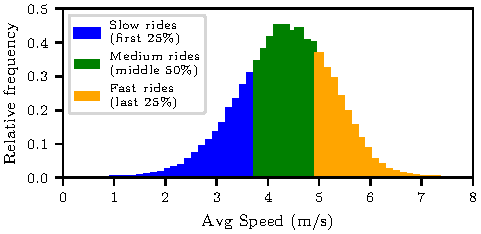
\includegraphics[width=0.7\columnwidth]{fig/analysis_avg_velo_all.pdf}
    \caption{%
        Histogram of the empirical average velocity capabilities of cyclists found in the SimRa dataset. The average velocity of all cycling trips after the preprocessing is \SI{4.38}{\metre\per\second} with a standard deviation of \num{0.89} and a median of \SI{4.42}{\metre\per\second}.
    }%
    \label{fig:analysis_avg_vel_all}
\end{figure}

\subsection{Acceleration}
\label{subsec:acceleration_preprocessing}
%  ____  _   _ __  __  ___                  ____  _           ____
% / ___|| | | |  \/  |/ _ \  __   _____    / ___|(_)_ __ ___ |  _ \ __ _
% \___ \| | | | |\/| | | | | \ \ / / __|   \___ \| | '_ ` _ \| |_) / _` |
%  ___) | |_| | |  | | |_| |  \ V /\__ \_   ___) | | | | | | |  _ < (_| |
% |____/ \___/|_|  |_|\___/    \_/ |___(_) |____/|_|_| |_| |_|_| \_\__,_|
\begin{figure*}
    %\vspace{-3em}
    \centering
    \subfloat[All cyclists]{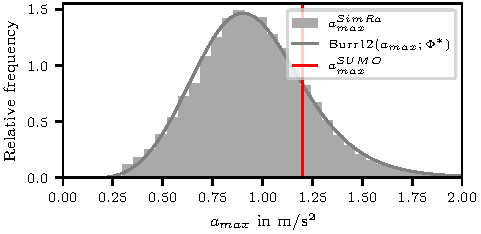
\includegraphics[width=0.4\columnwidth]{fig/analysis_max_acceleration_dist_fit_all.pdf}\label{fig:analysis_max_acceleration_dist_fit_all}}
    \hfill
    \subfloat[\num{3} cyclist groups: slow ($s$), medium ($m$), and fast ($f$)]{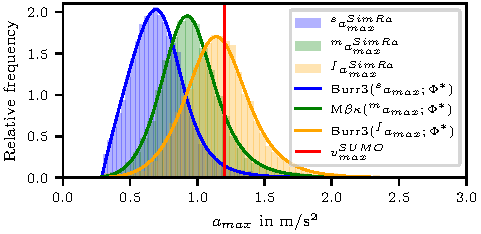
\includegraphics[width=0.4\columnwidth]{fig/analysis_max_acceleration_dist_fit_groups.pdf}\label{fig:analysis_max_acceleration_dist_fit_groups}}
    \caption{%
        Histogram of maximum acceleration capabilities found in the empirical SimRa dataset and their respective distribution functions.
        The red scalar represents the default value in \ac{sumo}.
    }%
    \label{fig:analysis_max_acceleration_dist_fit}
\end{figure*}

For analyzing cyclist acceleration, we extracted acceleration maneuvers from the dataset.
For this, we slightly adapted the approach of \cite{ma2016modeling}.
First, we split the velocity profile at its local extrema to get segments where the cyclist accelerates/decelerates.
Then, we consider only segments with a distance from \SI{20}{\metre} to \SI{350}{\metre} and a duration between \SI{5}{\second} to \SI{40}{\second}.
We also make sure to filter out segments where the variance in velocity is too low, i.e., such that $ \frac{|v_{s} - v_{e}|}{max(v_{s},v_{e})} > 0.5 $, where $v_{s}$ and $v_{e}$ are the velocities at the start and end of a segment.
With that approach we found \num{228347} acceleration maneuvers in the cleaned dataset.
Distribution fitting processes, which were done with SciPy\footnote{https://scipy.org/}, showed that the Burr (Type XII) distribution~\cite{burr1942cumulative} $Burr12(x; c,d) = c*d*\frac{x^{c-1}}{(1+x^c)^{d+1}}$ for $x = a_{max} \geq 0$ and $c,d > 0$  fits the data best for the general cyclist model (see also \Cref{fig:analysis_max_acceleration_dist_fit_all}).
For the models of the slow and fast cyclist models, the Burr (Type III) distribution~\cite{burr1942cumulative}

$Burr3(x; c,d) = c*d*\frac{x^{-c-1}}{(1+x^c)^{d+1}}$ for $x = a_{max} \geq 0$ and $c,d > 0$ fits the data best, while the Mielke Beta-Kappa distribution~\cite{mielke1973distribution}

$M\beta\kappa(x; c,d) = \frac{k*x^{k-1}}{(1+x^s)^{1+k/s}}$ for $x = a_{max} > 0$ and $k,s > 0$ is the best fit for the medium cyclist model's acceleration distribution (see also \Cref{fig:analysis_max_acceleration_dist_fit_groups}).

Comparing the acceleration capability of actual cyclists (the SimRa dataset) with the default \ac{sumo} cyclist model, differences become apparent.
By default, \ac{sumo} specifies $a_{max}^{\ac{sumo}}$ with \SI{1.2}{\metre\per\square\second}.
This deviates significantly from the findings in the SimRa dataset where only \num{15}\% of the acceleration maneuvers are executed with a maximum acceleration of \SI{1.2}{\metre\per\square\second} or higher.
Furthermore, the empirical distributions are rather wide, indicating a broad variance across different cyclist types and cycling situations, which is in stark contrast to \ac{sumo}'s strategy of choosing a fixed maximum value.

\subsection{Deceleration}
\label{subsec:deceleration_preprocessing}

%  ____  _   _ __  __  ___                  ____  _           ____
% / ___|| | | |  \/  |/ _ \  __   _____    / ___|(_)_ __ ___ |  _ \ __ _
% \___ \| | | | |\/| | | | | \ \ / / __|   \___ \| | '_ ` _ \| |_) / _` |
%  ___) | |_| | |  | | |_| |  \ V /\__ \_   ___) | | | | | | |  _ < (_| |
% |____/ \___/|_|  |_|\___/    \_/ |___(_) |____/|_|_| |_| |_|_| \_\__,_|
\begin{figure*}
    \centering
    \subfloat[All cyclists]{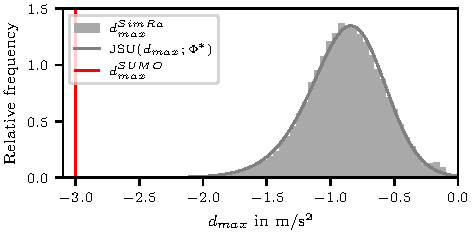
\includegraphics[width=0.4\columnwidth]{fig/analysis_max_deceleration_dist_fit_all.pdf}\label{fig:analysis_max_deceleration_dist_fit_all}}
    \hfill
    \subfloat[\num{3} cyclist groups: slow ($s$), medium ($m$), and fast ($f$)]{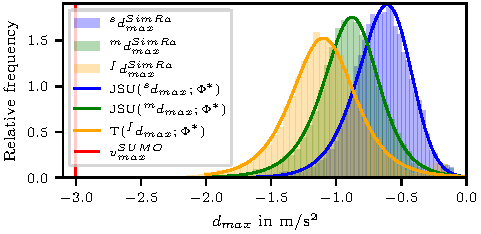
\includegraphics[width=0.4\columnwidth]{fig/analysis_max_deceleration_dist_fit_groups.pdf}\label{fig:analysis_max_deceleration_dist_fit_groups}}
    \caption{%
        Histogram of maximum deceleration capabilities found in the empirical SimRa dataset and their respective distribution functions.
        The red scalar represents the default value in \ac{sumo}.
    }%
    \label{fig:analysis_max_deceleration_dist_fit}
\end{figure*}

For analyzing cyclist deceleration, we extracted deceleration maneuvers from the dataset (see \Cref{subsec:acceleration_preprocessing}).
Distribution fitting processes showed here that the Johnson's $S_{U}$-distribution~\cite{johnson1949systems} $JSU(x; a,b) = \frac{b}{\sqrt{x^2+1}}\phi(a+b*log(x+\sqrt{x^2+1}))$ for $x=d_{max}$ and $b>0$ with $\phi$ being the probability density function of the normal distribution, fits the data best for the general cyclist model (see also \Cref{fig:analysis_max_deceleration_dist_fit_all}).
$JSU(d_{max}; a,b)$ was also the best fit for the slow and medium cylist models, whereas the fast cyclists' data was the best fit for the Student's $t$-distribution~\cite{student1908probable} $t(x; \nu)=\frac{\Gamma((\nu+1)/2)}{\sqrt{\pi*\nu}*\Gamma(\nu/2)}*(1+x^2/\nu)^{-(\nu+1)/2}$ for $x=d_{max}$ (see also \Cref{fig:analysis_max_deceleration_dist_fit_groups}).

Comparing the deceleration capability of actual cyclists (the SimRa dataset) with the default \ac{sumo} bicycle model, differences become apparent.
By default, \ac{sumo} specifies $d_{max}^{\ac{sumo}}$ with \SI{-3}{\metre\per\square\second}.
This deviates extremely from the findings in the SimRa dataset where none of the deceleration maneuvers are executed with a maximum acceleration of \SI{-3}{\metre\per\square\second} or lower.
Furthermore, the empirical distributions are rather wide, indicating a broad variance across different cyclist types and cycling situations, which is in stark contrast to \ac{sumo}'s strategy of choosing a fixed maximum value.

\subsection{Velocity}
\label{subsec:velocity_preprocessing}
%  ____  _   _ __  __  ___                  ____  _           ____
% / ___|| | | |  \/  |/ _ \  __   _____    / ___|(_)_ __ ___ |  _ \ __ _
% \___ \| | | | |\/| | | | | \ \ / / __|   \___ \| | '_ ` _ \| |_) / _` |
%  ___) | |_| | |  | | |_| |  \ V /\__ \_   ___) | | | | | | |  _ < (_| |
% |____/ \___/|_|  |_|\___/    \_/ |___(_) |____/|_|_| |_| |_|_| \_\__,_|

\begin{figure*}
    %\vspace{-3em}
    \centering
    \subfloat[All cyclists]{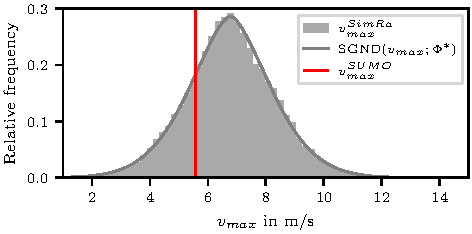
\includegraphics[width=0.4\columnwidth]{fig/analysis_max_velo_dist_fit_all.pdf}\label{fig:analysis_max_velo_dist_fit_all}}
    \hfill
    \subfloat[\num{3} cyclist groups: slow ($s$), medium ($m$), and fast ($f$)]{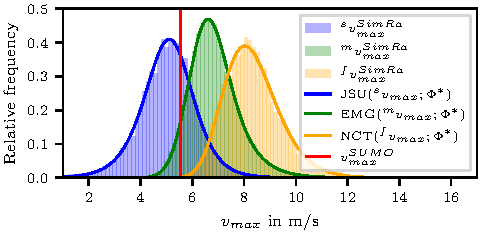
\includegraphics[width=0.4\columnwidth]{fig/analysis_max_velo_dist_fit_groups.pdf}\label{fig:analysis_max_velo_dist_fit_groups}}
    \caption{%
        Histogram of maximum velocity capabilities found in the empirical SimRa dataset and their respective distribution functions.
        The red scalar represents the default value in \ac{sumo}.
    }%
    \label{fig:analysis_max_velo_dist_fit}
    \vspace{-.5em}
\end{figure*}

To gain insights into cyclists' behavior regarding their velocities, we calculate the maximum velocity for each ride file in the cleaned SimRa dataset.
Using distribution fitting, we found that the symmetric generalized normal distribution~\cite{nadarajah2005generalized} $SGND(x;\beta) = \frac{\beta}{2*\Gamma(1/\beta)}*exp(-|x|^\beta)$ for $x=v_{max}$ fits the empirical data of all cyclists best (see also \Cref{fig:analysis_max_velo_dist_fit_all}) and is therefore a valid fit for the specification of the empirical distribution of $v_{max}^{SimRa}$ for the general cyclist model.
For the model of the slow cyclists, the Johnson's $S_{U}$-distribution~\cite{johnson1949systems} $JSU(v_{max}; \Phi\mbox{*})$ fits the data best, while the best fit for the medium cyclists' model is the Exponentially Modified Gaussian distribution~\cite{grushka1972characterization} $EMG(x; K) = \frac{1}{2*K}*exp(\frac{1}{2*K^2}-x/K)erfc(-\frac{x-1/K}{\sqrt{2}})$ for $x = v_{max}$ and $K>0$.
Finally, the non-central $t$-distribution~\cite{hogben1961moments} $NCT\newline(v_{max}; \Phi\mbox{*})$ emerged as the best fit for the fast cyclists' data.

On the other hand, \ac{sumo} sets $v_{max}^{\ac{sumo}}$ at \SI{5.56}{\metre\per\s} by default.
This deviates significantly from the findings in the SimRa dataset where \num{77}\% of the rides have a higher maximum velocity.
Bringing this together with the acceleration findings, real-world cyclists often (but not always) cycle much faster than \ac{sumo} cyclists and vary much more in their acceleration behavior.

\subsection{Left-turn Behavior at Intersections}
\label{subsec:left-turn_behavior_at_intersections_preprocessing}
%  ____  _   _ __  __  ___                  ____  _           ____
% / ___|| | | |  \/  |/ _ \  __   _____    / ___|(_)_ __ ___ |  _ \ __ _
% \___ \| | | | |\/| | | | | \ \ / / __|   \___ \| | '_ ` _ \| |_) / _` |
%  ___) | |_| | |  | | |_| |  \ V /\__ \_   ___) | | | | | | |  _ < (_| |
% |____/ \___/|_|  |_|\___/    \_/ |___(_) |____/|_|_| |_| |_|_| \_\__,_|
\begin{figure}
    \centering
    \includegraphics[width=0.5\columnwidth]{fig/analysis_im_loc_default.pdf}
    \caption{%
        Qualitative comparison between the \ac{sumo} default intersection model and real world data given by SimRa for the intersection between Alexanderstraße and Karl-Marx-Allee in Berlin.
        SimRa shows two distinct left-turn paths (i.e., a direct and an indirect one) whereas \ac{sumo} default only models the direct path.
    }%
    \label{fig:analysis_im_traj_default}
\end{figure}

According to the SimRa dataset, cyclists either behave like cars (using the normal road) or pedestrians (using the pedestrian crossing) to take left-turns at intersections.
We call the former a \textit{direct} left turn and the latter an \textit{indirect} left turn.

\ac{sumo}'s default model only provides cyclists with an unrealistic "bicycle-lane-to-bicycle-lane-left-turn" (see also \Cref{fig:analysis_im_traj_default}), where the cyclist enters the intersection from a bicycle lane, crossing all car lanes and directly entering the bicycle lane again.

Taking a closer look at real world intersections in the SimRa dataset revealed that there are mainly two intersection types.
In the first intersection type, the \textit{indirect} path is chosen with a probability of \num{61}\% when all cyclists are considered, while medium cyclists and fast cyclists prefer the indirect path with a probability of \num{87}\% and \num{50}\% respectively.
However, on the second intersection type, almost all cyclists choose the \textit{indirect} path.
Slow cyclists almost never tend to do direct left-turns, since they presumably avoid car traffic the most.
Randomly investigating intersections of both types revealed that the first intersection type has no specific characteristics while the second intersection type actively encourages cyclists to indirect turns through the design of the intersection, e.g., by having a traffic island in the center.
Since such information cannot be identified in \ac{osm} data reliably and in an abstract way, we will consider only the first intersection type in the following.

\ac{sumo} and real world data differ decisively in all metrics considered, namely acceleration, velocity, and left-turn behavior at intersections.
However, these three metrics are crucial for realistically simulating bicycle traffic.
In the following, we try to adapt \ac{sumo} to simulate a more realistic cyclist behavior by introducing three different cyclist types.


\section{Improving \ac{sumo}'s Bicycle Simulation}
\label{sec:improving_sumos_bicycle_simulation}
To improve the simulation, we propose three changes to \ac{sumo}'s bicycle model:
First, the longitudinal kinematic parameters of \ac{sumo}'s default bicycle model are \mbox{(re-)}parameterized based on the findings from the SimRa dataset.
Second, a novel simulation model is derived from SimRa trajectories to exclusively simulate realistic left-turn bicycle behavior at intersections based on the findings in \Cref{sec:cycling_behavior_in_simra_and_sumo}.
The latter model is referred to as the intersection model in the following.
Third, four different cyclist models, with different longitudinal kinematic and left-turn behaviors depending on the findings from \Cref{sec:cycling_behavior_in_simra_and_sumo}.
One model is for all cyclists combined and the three other models are for modeling slow, medium and fast cyclists.


\subsection{Longitudinal Kinematic Behavior}
\label{subsec:longitudinal_kinematic_behavior}
In \Cref{sec:cycling_behavior_in_simra_and_sumo}, we derived maximum acceleration, maximum deceleration and maximum velocity characteristics from the SimRa dataset.
We now use them to improve the longitudinal kinematic behavior of the default \ac{sumo} bicycle model.
Contrary to the default parameterization, we use theoretical distribution functions instead of scalar values for the exposed kinematic parameters.
This enables the model to produce more realistic bicycle simulation results since the heterogeneity of real world cycling styles is reflected.

We derive the theoretical distributions by aggregating the respective features from \Cref{subsec:acceleration_preprocessing,subsec:deceleration_preprocessing,subsec:velocity_preprocessing}.
For this, we rely on the \textit{law of large numbers} which states that the average of the results obtained from a large number of trials of the same experiment eventually converges to its true expected value~\cite{etemadi1981elementary}.
In the context of this work, this means that individual rides do not matter but that the aggregates of multiple rides will converge towards their actual expected value given a sufficiently large number of rides.

For the implementation, we used \textit{vTypeDistributions} following the results of our previous analysis and sample both distribution independently.

It should be noted that through the parameterizations with theoretical probability density functions \ac{sumo}'s \textit{speedDev} parameter becomes obsolete as variance between the kinematic preferences among cyclists are already represented by the distribution function.

Furthermore, alternatives for the acceleration parameters have been added to \ac{sumo}. This would enable a user to pick a normal distribution and choose the parameters for it.
This is would yield more realistic scenario data contrary to using a simple scalar value for the acceleration.

\subsection{Left-turn Behavior at Intersections}
\label{subsec:left-turn_behavior_at_intersections}
To improve the degree of realism in cyclists' left-turn behavior at signaled intersections, we use an adapted version of the external intersection model (a Python script that steers cyclists via \ac{sumo}'s \textit{Traffic Control Interface}) as proposed by \textcite{kaths2016integration} which is based on previously recorded real-world trajectories as their guidelines for cyclists across a single predefined intersection.
Our approach algorithmically synthesizes the cyclists' trajectories (i.e., their respective guidelines across the intersection) for any regular four-way intersection and can therefore be seen as a step towards a more universal solution.

The left-turn maneuver distribution, as we call it, specifies the probability of the cyclists choosing either the \textit{direct} or the \textit{indirect} path to cross the intersection.
For this, we use the distributions derived in \Cref{subsec:left-turn_behavior_at_intersections_preprocessing} as the default for our intersection model for each different cyclist group.
Users, however, can adjust the distributions if desired or needed for their specific purposes (see also the exception cases in \Cref{subsec:left-turn_behavior_at_intersections_preprocessing}).

In order to simplify the process and to improve performance, we decided to integrate this feature into the \ac{sumo} core.
The implementation provides a new parameter that lets the user adjust the indirect left turn probability of a cycling trip.
To detail the workflow, the cyclist makes a decision before each intersection, where there is at least one direct and indirect left-turn available to choose from.
This delegates decisions inside \ac{sumo} just by using the bicycle vehicle type parameter.

\subsection{Different Cyclist Models}
\label{subsec:different_cyclist_models}

Our approach defines distibutions of models derived from the same default implementation of \ac{sumo}.
The models vary only in the parameter values used.
The parameters considered are maximum acceleration (\textit{accel}), maximum deceleration (\textit{decel}) and maximum velocity (\textit{maxSpeed}), splitted into \num{3} groups, as it can be seen in \Cref{subsec:acceleration_preprocessing,subsec:deceleration_preprocessing,subsec:velocity_preprocessing}.
In order to leverage distribution parameters for a bicycle model, we used the \textit{vTypeDistribution} from \ac{sumo} to define a distribution of cyclists having all the parameters mentioned.

With this data ready, the only remaining step is to augment these groups with a left-turn behavior probability per group.
In order to make a decision whether to do a direct or an indirect left-turn, we approached the problem by using a script that controls the cyclists, as described in \Cref{subsec:left-turn_behavior_at_intersections}.

Thus, this group-based model enables the user to simulate bicycle traffic in \ac{sumo} more realistically.

\section{Evaluation}
\label{sec:evaluation_sumo}
In this section, we evaluate the new cyclist models from \Cref{sec:improving_sumos_bicycle_simulation} by comparing them to each other and to \ac{sumo}'s default simulation model and the real-world data taken from the SimRa data set.
We start by introducing the simulation setup (\Cref{subsec:simulation_setup}) which we used to create and run the scenarios with.
We then continue analyzing acceleration (\Cref{subsec:acceleration_evaluation}), deceleration (\Cref{subsec:deceleration_evaluation}), velocity (\Cref{subsec:velocity_evaluation}), and left-turn behavior at intersections (\Cref{subsec:left-turn_behavior_at_intersections_evaluation}) before evaluating the combination of all model extensions (\Cref{subsec:combinin_intersection_model_and_kinematic_extension}).
Please note: While it may appear obvious that using the SimRa data set for both parameterization and evaluation should lead to perfect results, this is not the case as our extensions are subject to the design restrictions imposed by \ac{sumo}

\subsection{Simulation Setup}
\label{subsec:simulation_setup}
% scenarios
As \ac{sumo} users can import real-world scenarios from OSM data, simulation results can be compared to real-world data and thus be evaluated.
For our evaluation, we chose specific traffic scenarios from multiple SimRa regions that are representative and likely to showcase both strengths and weaknesses of our extensions.
Likewise, we do not show every cyclist type's results in detail to avoid too many figures and tables.
For evaluating the longitudinal behavior (acceleration, deceleration and velocity), we chose urban traffic scenarios with long straight sections.
As example locations, we use \textit{Oranienstraße} in Berlin, \textit{Dachauer Straße} in Munich and \textit{Frauentorgraben} in Nuremberg.
For evaluating left-turn behavior, we chose compact scenarios around signaled intersections with multiple lanes on each axis.
For this, we study three intersections in Berlin, namely at \textit{Mehringdamm} (see also \Cref{fig:mehringdamm_sumo}), \textit{Warschauer Straße}, and \textit{Alexanderstraße}.

\begin{table}%
\centering
\caption{Most important attributes of our simulation scenarios.}%
\label{tab:scenarios}
%\resizebox{\columnwidth}{!}{
\begin{tabular}{ccccc}%
\toprule%
                & Cars  & Bicycles & Distance & Lanes\\%
\midrule%
\midrule%
Oranienstr.     & \num{3158} & \num{300}      & \num{1528}    & --\\%
Dzchauer Str.   & \num{3427} & \num{300}      & \num{1204}    & --\\%
Frauentorgraben & \num{1625} & \num{300}      & \num{1023}    & --\\%
Mehringdamm     & \num{180}   & \num{2700}    & --       & \num{29}\\%
Warschauer Str. & \num{180}   & \num{2700}    & --       & \num{26}\\%
Alexanderstr.   & \num{180}   & \num{2700}    & --       & \num{25}\\%
\bottomrule&%
\end{tabular}%
%}
\end{table}

We made our scenarios as realistic as possible by choosing main roads and intersections with a lot of traffic and also added a significant number of cars, as \Cref{tab:scenarios} shows.
\begin{figure}
    \centering
    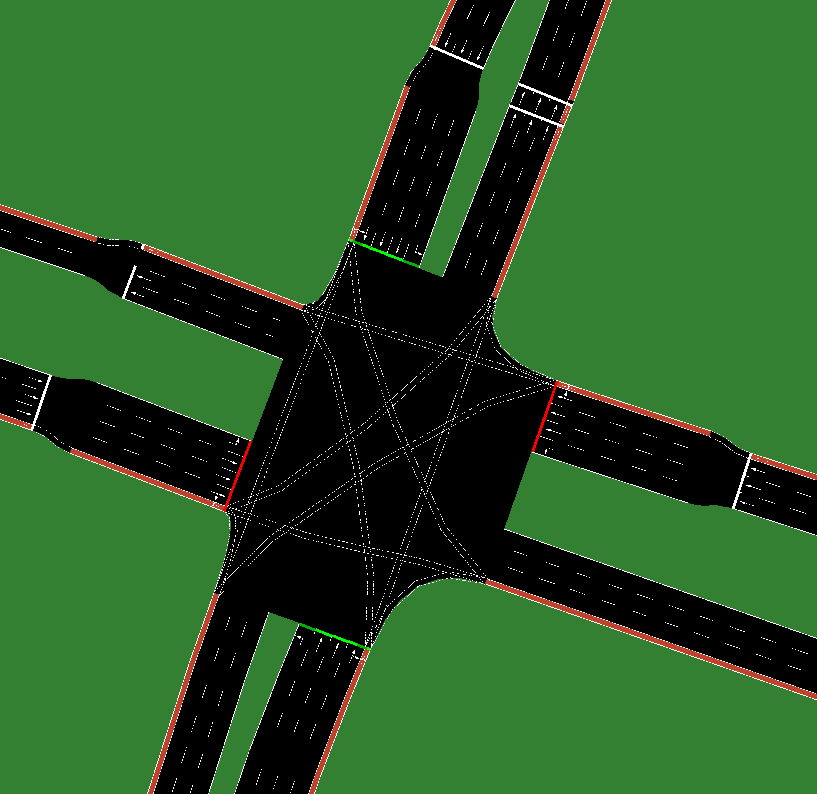
\includegraphics[width=0.5\columnwidth]{fig/mehringdamm_screenshot.png}
    \caption{%
        Excerpt from the \textit{Mehringdamm} scenario in \ac{sumo}.
        The scenario was created using OSM data only.
    }%
    \label{fig:mehringdamm_sumo}
\end{figure}

% simulation and environment and parameterization
For our evaluation, we use \ac{sumo} version 1.14.0 and a step size of \SI{1}{\s} in simulations.
The \ac{sumo} default results are obtained with \ac{sumo}'s \textit{vType} \texttt{Bicycle} for cyclists, i.e., the maximum acceleration, maximum deceleration and maximum velocity are scalars and set to \SI{1.2}{\m\per\s\squared}, \SI{-3}{\m\per\s\squared} and \SI{5.56}{\m\per\s} respectively.

\subsection{Acceleration}
\label{subsec:acceleration_evaluation}
\begin{figure*}
    \vspace{-1.5em}
    \centering
    \subfloat[All cyclists]{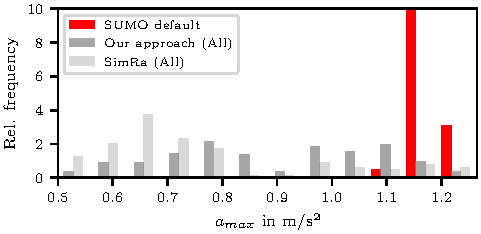
\includegraphics[width=0.4\columnwidth]{fig/eval_acc_all.pdf}\label{fig:eval_acc_all}}
    \hfill
    \subfloat[Only cyclist group slow ($s$)]{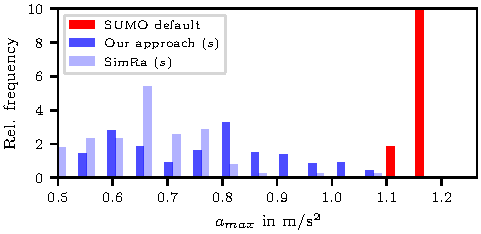
\includegraphics[width=0.4\columnwidth]{fig/eval_acc_slow.pdf}\label{fig:eval_acc_slow}}
    \caption{%
        Histogram of \ac{sumo}'s, SimRa's, and our approach's observed maximum accelerations inside the example \textit{Frauentorgraben} scenario.
        While the maximum accelerations are heterogeneously distributed in the real-world data and our approach, the default values are clustered.
        Here, the observed accelerations deviate from the configured default value (\SI{1.2}{\metre\per\square\second}) due to traffic effects inside the simulation.
    }%
    \label{fig:eval_acc}
\end{figure*}

\Cref{fig:eval_acc_all} shows the empirical distributions of the maximum acceleration among all cyclist types inside the \textit{Frauntorgraben} scenario simulation and the corresponding real world data.
It is evident that real-world acceleration maneuvers show heterogeneous maximum rates of acceleration.
The same is true for the three cyclist groups of our new approach as \Cref{fig:eval_acc_slow} shows.
Note that the other two cyclist groups, namely slow and medium, allow the same conclusion and, that we have randomly chosen the slow cyclist group to visualize in \Cref{fig:eval_acc_slow} to make the figure more readable.
Apparently, the default parameterization is not suitable to describe this acceleration behavior among cyclists, as it provides homogeneous maximum acceleration rates within the simulation.
Our new parameterization - for all cyclists together and for each of the cyclist types - is significantly closer to the real-world behavior in the SimRa data set with its highly heterogeneous behavior across cyclists.
\begin{table}
\centering
\caption{Results Overview Maximum Acceleration Comparing \ac{sumo} Default, Our Approach (All), Our Approach (Slow), SimRa (All) and SimRa (Slow)}%
\label{tab:results_overview_acc}
\begin{tabular}{cccc}
\toprule
& Mean & Std. Deviation & Median\\
\midrule
\midrule
\ac{sumo} default & \num{1.178} & \num{0.019} & \num{1.18} \\
\midrule
Our approach (\textit{all}) & \num{0.921} & \num{0.218} & \num{0.95} \\
SimRa (\textit{all}) & \num{0.761} & \num{0.217} & \num{0.71} \\
\midrule
Our approach (\textit{s}) & \num{0.727} & \num{0.168} & \num{0.74} \\
SimRa (\textit{s}) & \num{0.656} & \num{0.109} & \num{0.65} \\
\bottomrule&
\end{tabular}
\end{table}
This can also be seen, when comparing the mean, standard deviation and median values of \ac{sumo} default, all and slow (\textit{s}) cyclists (both in the SimRa dataset and our approach) depicted in \Cref{tab:results_overview_acc}.
It also shows, that the division of the cyclist into subgroups further increases the realism, since the difference between the mean and median values of our approach (\textit{all}) and Simra (\textit{all}) shrinks, compared to our approach (\textit{s}) and Simra (\textit{s}).
The standard deviation suffers though, which is probably due to less rides being regarded, because of the splitting into three subgroups.
Please note also here, that we omitted the medium and fast cycling groups to stay consistent with \Cref{fig:eval_acc_slow} and avoid clutter.
That our new parameterizations are not a perfect fit indicates that there are probably additional influence factors, e.g., the traffic density or the weather situation, not covered in our kinematic models which aggregate data from all SimRa rides.

\subsection{Deceleration}
\label{subsec:deceleration_evaluation}
\begin{figure*}
    %\vspace{-3em}
    \centering
    \subfloat[All cyclists]{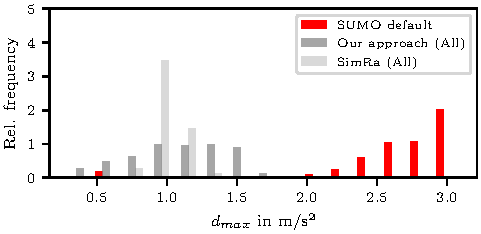
\includegraphics[width=0.4\columnwidth]{fig/eval_dec_all.pdf}\label{fig:eval_dec_all}}
    \hfill
    \subfloat[Only cyclist group medium ($m$)]{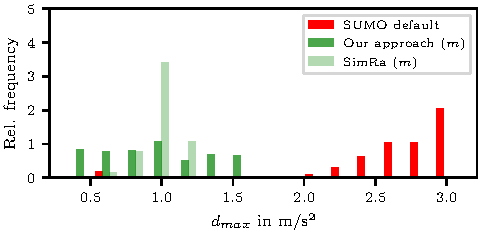
\includegraphics[width=0.4\columnwidth]{fig/eval_dec_medium.pdf}\label{fig:eval_dec_medium}}
    \caption{%
        Histogram of \ac{sumo}'s, SimRa's, and our approach's observed maximum decelerations inside the example \textit{Dachauer Straße} scenario.
        While the maximum decelerations are heterogeneously distributed in the real-world data and our approach, the default values are clustered.
        Here, the observed decelerations deviate from the configured default value (3m/s\textsuperscript{2}) due to traffic effects inside the simulation.
    }%
    \label{fig:eval_dec}
\end{figure*}

\Cref{fig:eval_dec_all} shows the empirical distributions of the maximum deceleration among all cyclist types inside the \textit{Dachauer} \textit{Straße} scenario simulation and the corresponding real world data.
Here, we only show the medium cyclist group as an example to avoid clutter, the other two cycling groups (slow and fast) show very similar results.
It is evident that real-world deceleration maneuvers show heterogeneous maximum rates of deceleration.
The same is true for the medium cyclists as \Cref{fig:eval_dec_medium} shows.
Here, too, the default parameterization is not suitable to describe this deceleration behavior among cyclists, as it provides homogeneous maximum deceleration rates within the simulation.
Our new parameterization - for all cyclists together and for each of the cyclist types - is significantly closer to the real-world behavior in the SimRa data set with its highly heterogeneous behavior across cyclists.
\begin{table}
\centering
\caption{Results Overview Maximum Deceleration Comparing \ac{sumo} Default, Our Approach (All), Our Approach (Medium), SimRa (All) and SimRa (Medium)}%
\label{tab:results_overview_dec}
\begin{tabular}{cccc}
\toprule
& Mean & Std. Deviation & Median\\
\midrule
\midrule
\ac{sumo} default & \num{2.664} & \num{0.507} & \num{2.77} \\
\midrule
Our approach (\textit{all}) & \num{1.071} & \num{0.336} & \num{1.09} \\
SimRa (\textit{all}) & \num{0.962} & \num{0.141} & \num{0.96} \\
\midrule
Our approach (\textit{m}) & \num{0.949} & \num{0.362} & \num{0.93} \\
SimRa (\textit{m}) & \num{0.973} & \num{0.100} & \num{0.98} \\
\bottomrule&
\end{tabular}
\end{table}
Just like with the maximum acceleration, \Cref{tab:results_overview_dec} shows, that our approach is not only more realistic than \ac{sumo}'s default bicycle model (both with all and medium (\textit{m}) cyclists), but the introduction of the cyclist groups increases the realism.
The medium cyclist group was randomly chosen as a representative for the other groups, since the conclusion does not differ.
Influence factors, such as the traffic density or the weather situation, not covered in our kinematic models which aggregate data from all SimRa rides, result in a non-perfect fit for our new parameterizations.
Note, that we had to filter out deceleration values, that we deemed too high (above \SI{7}{\m\per\s\squared}), to avoid recording emergency deceleration, which is another parameter in \ac{sumo}'s vehicle parameterization.

\subsection{Velocity}
\label{subsec:velocity_evaluation}
\begin{figure*}
    \centering
    \subfloat[All cyclists]{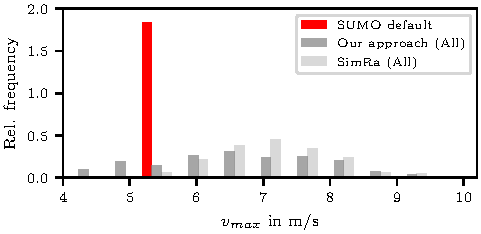
\includegraphics[width=0.4\columnwidth]{fig/eval_velo_all.pdf}\label{fig:eval_velo_all}}
    \hfill
    \subfloat[Only cyclist group fast ($f$)]{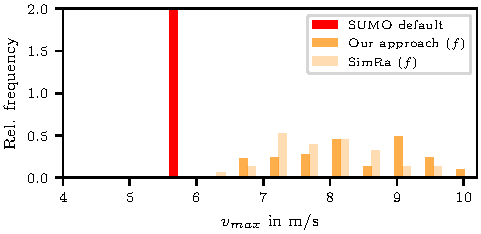
\includegraphics[width=0.4\columnwidth]{fig/eval_velo_fast.pdf}\label{fig:eval_velo_fast}}
    \caption{%
        Histogram of \ac{sumo}'s, SimRa's, and our approach's observed maximum velocities inside the example \textit{Oranienstraße} scenario.
        While the maximum velocities are heterogeneously distributed in the real-world data and our approach, the default values are clustered.
    }%
    \label{fig:eval_velo}
\end{figure*}

\Cref{fig:eval_velo_all} shows the empirical distributions of all cyclists' maximum velocities in the \textit{Oranienstraße} scenario simulation and the real-world scenario.
As with maximum acceleration and deceleration rates, maximum velocities vary widely among real-world cyclists and we only depict one cyclist group (this time fast cyclists) as an example for other groups to increase the readability of the figure.
Once more, the default parameterization is not able to reflect this characteristic.
This is also the case for the different cyclist groups as \Cref{fig:eval_velo_fast} shows exemplary.
\begin{table}
\centering
\caption{Results Overview Maximum Velocity Comparing \ac{sumo} Default, Our Approach (All), Our Approach (Fast), SimRa (All) and SimRa (Fast)}%
\label{tab:results_overview_vel}
\begin{tabular}{cccc}
\toprule
& Mean & Std. Deviation & Median\\
\midrule
\midrule
\ac{sumo} default & \num{5.555} & \num{0.002} & \num{5.556} \\
\midrule
Our approach (\textit{all}) & \num{6.589} & \num{1.234} & \num{6.58} \\
SimRa (\textit{all}) & \num{7.072} & \num{0.904} & \num{7.10} \\
\midrule
Our approach (\textit{f}) & \num{8.272} & \num{0.902} & \num{8.20} \\
SimRa (\textit{f}) & \num{7.872} & \num{0.738} & \num{7.86} \\
\bottomrule&
\end{tabular}
\end{table}
According to \Cref{tab:results_overview_vel} the maximum velocity aspect of our simulation is the closest, when compared to maximum acceleration and maximum deceleration of all and fast (\textit{f}) cyclist groups in SimRa and our approach.
This is probably due to the fact, that we splitted the cyclist based on the average velocity.
Our new parameterization is thus significantly closer to the real-world behavior of cyclists.
As for acceleration and deceleration behaviors, the fact that our new parameterization is not a perfect fit to the real-world data indicates that there are likely to be additional influence factors not captured in our model.

\subsection{Left-turn Behavior at Intersections}
\label{subsec:left-turn_behavior_at_intersections_evaluation}

%  _   _ _______        __                ____  _           ____
% | \ | | ____\ \      / / __   _____    / ___|(_)_ __ ___ |  _ \ __ _
% |  \| |  _|  \ \ /\ / /  \ \ / / __|   \___ \| | '_ ` _ \| |_) / _` |
% | |\  | |___  \ V  V /    \ V /\__ \_   ___) | | | | | | |  _ < (_| |
% |_| \_|_____|  \_/\_/      \_/ |___(_) |____/|_|_| |_| |_|_| \_\__,_|
\begin{figure*}
    \centering
    \subfloat[Only cyclist group slow ($s$)]{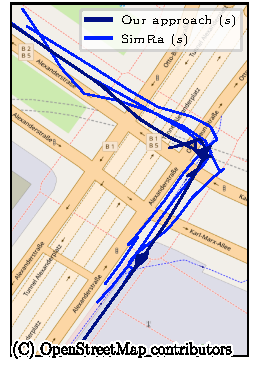
\includegraphics[width=.25\textwidth]{fig/eval_im_loc_im_slow.pdf}\label{fig:eval_im_traj_slow}}
    \hfill
    \subfloat[Only cyclist group medium ($m$)]{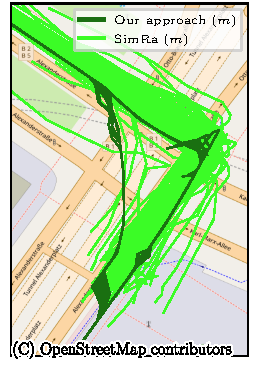
\includegraphics[width=.25\textwidth]{fig/eval_im_loc_im_medium.pdf}\label{fig:eval_im_traj_medium}}
    \hfill
    \subfloat[Only cyclist group fast ($f$)]{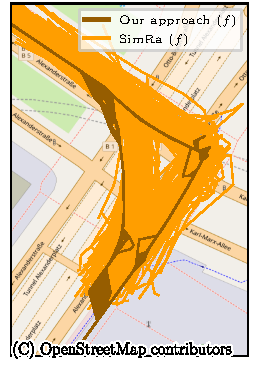
\includegraphics[width=.25\textwidth]{fig/eval_im_loc_im_fast.pdf}\label{fig:eval_im_traj_fast}}
    \caption{%
        Qualitative comparison between the results of our approach for the intersection model and real-world raw GPS data given by SimRa for the intersection between Alexanderstraße and Karl-Marx-Allee in Berlin.
        SimRa shows two distinct left-turn paths (i.e., a direct and an indirect one), which are also modeled by our models.
        Also the three different groups have different shares between direct and indirect left-turns.
    }%
    \label{fig:eval_im_traj_new}
\end{figure*}

As shown in \Cref{fig:eval_im_traj_new}, which shows the intersection between Alexanderstraße and Karl-Marx-Allee in Berlin, the 2D trajectories produced by the new intersection models converge towards the trajectories of the SimRa data set.
While the trajectories produced by \ac{sumo}'s default bicycle model, as can be seen in \Cref{fig:analysis_im_traj_default}, only offer direct "bike-lane-to-bike-lane" turns, the new model is significantly closer to real-world intersection behavior of cyclists.
This is true for all of our cyclist models.
Here, we see again the different left-turn behaviors of different cyclist types.
While slow cyclist only prefer the indirect left-turn, the medium and fast cyclists are more inclined to take the direct left-turn comparatively.

\subsection{Combining Intersection Model and Kinematic Extension}
\label{subsec:combinin_intersection_model_and_kinematic_extension}
To achieve a holistic comparison between \ac{sumo}'s default bicycle model and our new models, we measure the durations of left-turn maneuvers at multiple intersections and compare the empirical distributions of these measurements.
To specifically monitor the impact of our changes, we do not include any ride time before or after the intersection in the measurements.
Note that we also omit the slow rides, since no or too few slow rides went through the intersections presented here.

Based on this, we identified the following four findings:
%% BEST MATCH
% __        ___    ____  ____   ____ _   _    _   _   _ _____ ____
% \ \      / / \  |  _ \/ ___| / ___| | | |  / \ | | | | ____|  _ \
%  \ \ /\ / / _ \ | |_) \___ \| |   | |_| | / _ \| | | |  _| | |_) |
%   \ V  V / ___ \|  _ < ___) | |___|  _  |/ ___ \ |_| | |___|  _ <
%    \_/\_/_/   \_\_| \_\____/ \____|_| |_/_/   \_\___/|_____|_| \_\
\begin{figure}
    \centering
    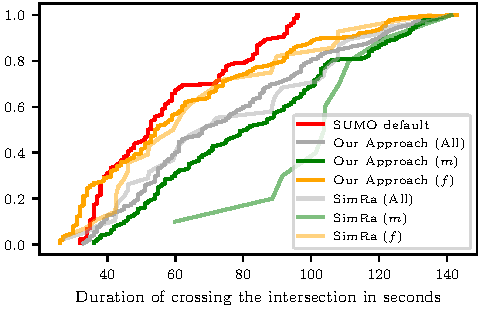
\includegraphics[width=0.7\columnwidth]{fig/im_warschauer_ecdf_every.pdf}
    \caption{%
        ECDFs of the measured durations for crossing the scenario \textit{Warschauer Straße}.
        It is apparent that our models for all, medium ($m$) and fast ($f$) cyclists outperform \ac{sumo}'s default as the measured durations converge towards the real-world data.
        Only our fast cyclist model ($f$) is just marginally better than \ac{sumo}'s default.
    }%
    \label{fig:im_warschauer}
\end{figure}
First, our new models outperform the default at most intersections, as its measured durations converge with real data, see for example \Cref{fig:im_warschauer}.
Especially when given the option to use the \textit{indirect} path, cyclists take longer to cross an intersection as they need to stop at an additional traffic light.
This is consistent with real-world data as we find it in the SimRa dataset at multiple intersections.

%% QUITE GOOD MATCH
%  __  __ _____ _   _ ____  ___ _   _  ____ ____    _    __  __ __  __
% |  \/  | ____| | | |  _ \|_ _| \ | |/ ___|  _ \  / \  |  \/  |  \/  |
% | |\/| |  _| | |_| | |_) || ||  \| | |  _| | | |/ _ \ | |\/| | |\/| |
% | |  | | |___|  _  |  _ < | || |\  | |_| | |_| / ___ \| |  | | |  | |
% |_|  |_|_____|_| |_|_| \_\___|_| \_|\____|____/_/   \_\_|  |_|_|  |_|
\begin{figure}
    \centering
    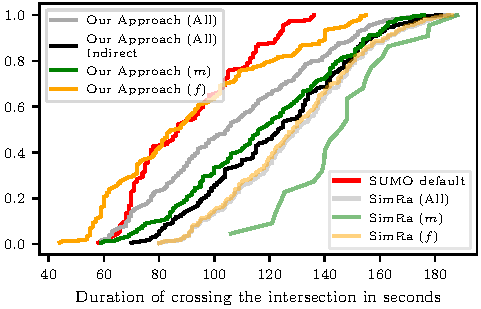
\includegraphics[width=0.7\columnwidth]{fig/im_mehringdamm_ecdf_every.pdf}
    \caption{%
        ECDFs of the measured durations for crossing the scenario \textit{Mehringdamm}.
        The results when using our models for all, medium ($m$) and fast ($f$) cyclists are only slightly more realistic than when using the standard \ac{sumo} model.
        However, when the \textit{direct} path is blocked for cyclists, the simulation results outperform the default approach.
    }%
    \label{fig:im_mehringdamm}
\end{figure}

Second, in some cases, we were able to improve our results by adjusting the left-turn behavior distribution following the second distribution discussed in \Cref{subsec:left-turn_behavior_at_intersections_preprocessing}.
The ``lane only'' results in \Cref{fig:im_mehringdamm} were achieved by prohibiting cyclists from using the \textit{direct} path.
Obviously, it takes much longer for cyclists to cross the intersection than \ac{sumo}'s default simulation model suggests.
When examining SimRa trajectories at this particular intersection, almost all cyclists chose the \textit{indirect} path as the infrastructure guides cyclists to do so.
Hence, manually adjusting the left-turn behavior distribution for such intersections is crucial.

%% NOT A GOOD MATCH
%     _    _     _______  __    _    _   _ ____  _____ ____
%    / \  | |   | ____\ \/ /   / \  | \ | |  _ \| ____|  _ \
%   / _ \ | |   |  _|  \  /   / _ \ |  \| | | | |  _| | |_) |
%  / ___ \| |___| |___ /  \  / ___ \| |\  | |_| | |___|  _ <
% /_/   \_\_____|_____/_/\_\/_/   \_\_| \_|____/|_____|_| \_\
\begin{figure}
    \centering
    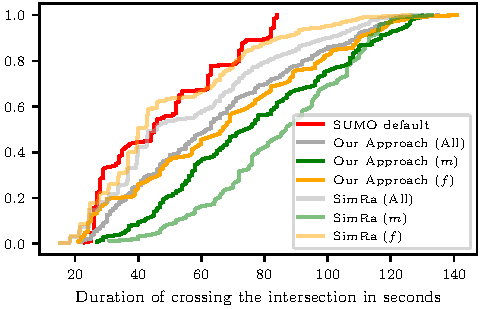
\includegraphics[width=0.7\columnwidth]{fig/im_alex_ecdf_every.pdf}
    \caption{%
        ECDFs of the measured durations for crossing the scenario \textit{Alexanderstraße}.
        Here, our new approach is not more precise than \ac{sumo} default behavior.
    }%
    \label{fig:im_alex}
\end{figure}

Third, at a few intersections, the results of our approach do not yet sufficiently reflect real-world bicycle behavior (see \Cref{fig:im_alex}).
We discuss possible reasons for this in \Cref{sec:discussion_sumo}.

Fourth, creating three cyclist models based on their average velocity also revealed, that \ac{sumo}'s default model behaves like fast cyclists.
This becomes clear when looking at \Cref{fig:im_warschauer,fig:im_mehringdamm,fig:im_alex}, since the lines representing the cyclists modeled with our fast cyclist model are the closes to the red line representing \ac{sumo} default.


\section{Discussion}
\label{sec:discussion_sumo}
Overall, the results presented in this chapter show a significant improvement over the state-of-the-art.
Nevertheless, they still have a number of shortcomings.
In this section, we discuss the inherent limitations of our approach in general (\Cref{subsec:methodological_challenges_sumo}) as well as problems resulting from the SimRa dataset as our ground truth data (\Cref{subsec:dataset_choice_as_ground_truth}).
We also describe a potential problem regarding e-bikes in \Cref{subsec:e-bikes}.
Note that we also discuss some limitations in \Cref{cha:discussion_and_outlook}, that may also apply to this approach.

%  __  __ _____ _   _ ____  ___ _   _  ____ ____    _    __  __ __  __
% |  \/  | ____| | | |  _ \|_ _| \ | |/ ___|  _ \  / \  |  \/  |  \/  |
% | |\/| |  _| | |_| | |_) || ||  \| | |  _| | | |/ _ \ | |\/| | |\/| |
% | |  | | |___|  _  |  _ < | || |\  | |_| | |_| / ___ \| |  | | |  | |
% |_|  |_|_____|_| |_|_| \_\___|_| \_|\____|____/_/   \_\_|  |_|_|  |_|
\begin{figure}
    \centering
    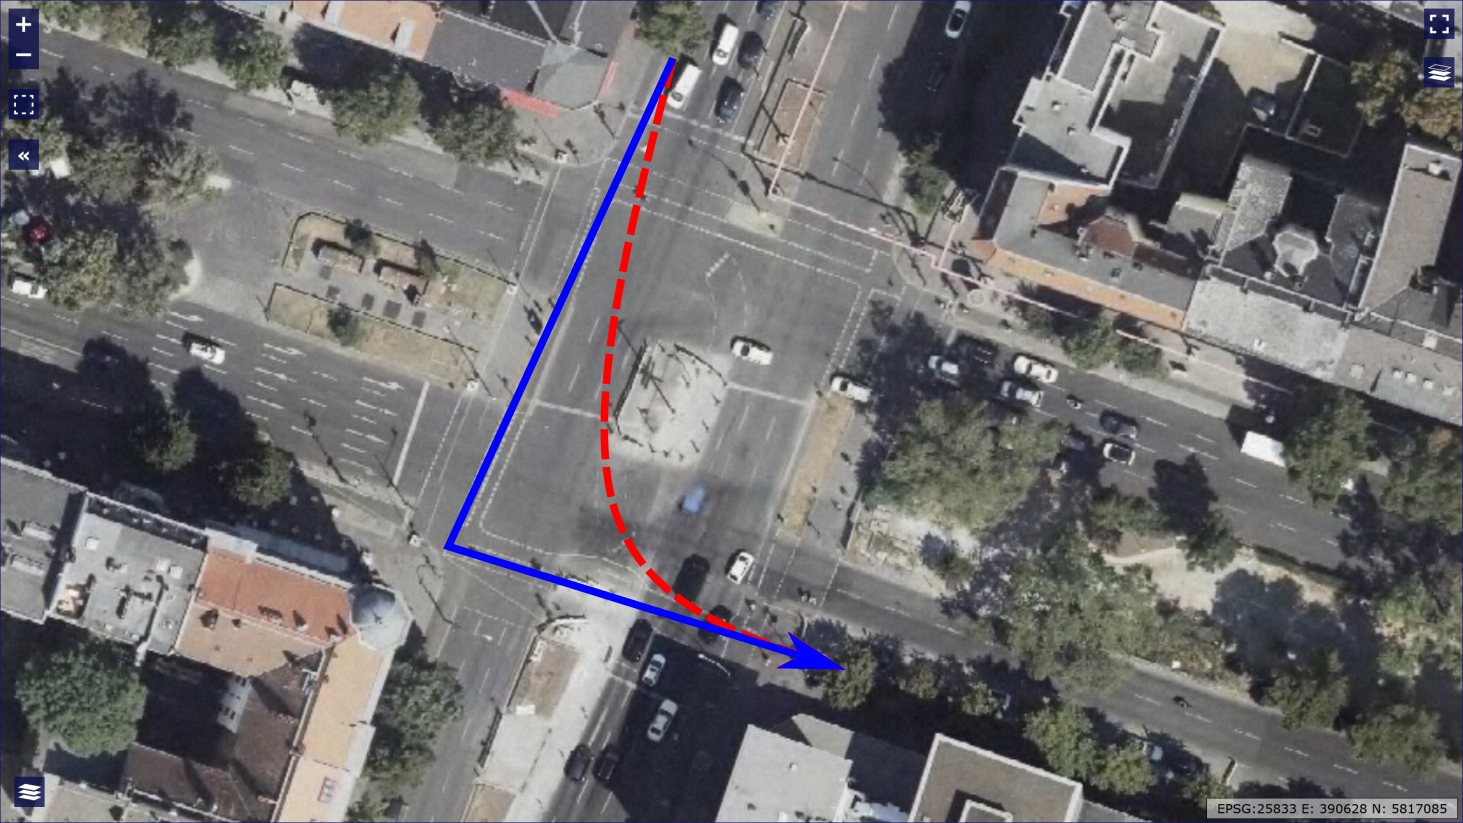
\includegraphics[width=0.7\columnwidth]{fig/mehringdamm_island_arrows.png}
    \caption{Intersection Mehringdamm/Gneisenaustraße: a traffic island obstructs the direct turn path (dashed line) and, thus, makes the indirect path (solid line) more likely to be used.}
    \label{fig:mehringdamm_traffic_island}
\end{figure}

\subsection{Methodological Challenges}
\label{subsec:methodological_challenges_sumo}
%Generalization Problem
%\paragraph{Generalizing Behavior}
Our initial assumption was that the behavior of cyclists in a single intersection cannot be generalized to all intersections~\cite{kaths2016integration} but that the average behavior across a large number of intersections will be close enough to cyclists' behavior at arbitrary intersections.
This seems to be true only for a (relatively large) subset of intersections -- apparently, the intersection behavior of cyclists is more heterogeneous than expected.
We believe that this is due to the fact that we averaged across all intersections in our dataset whereas there are apparently different classes of intersections that we did not account for.

Primarily, the intersection design is likely to have a strong impact:
Consider the example in \Cref{fig:mehringdamm_traffic_island} where a traffic island partially blocks direct left turns and where markings on the ground suggest indirect turns.
As another example, the intersection Bismarckstraße/Leibnizstraße had no direct left turns in the SimRa dataset.
In this intersection, the reason would be that cyclists legally have to use a bike lane.
When using that bike lane, a direct left turn would require cyclists to first pass through a row of parked cars, then to cross four car lanes of a major street before being able to turn left.

Aside from that, other possible influence factors include the amount and velocity of traffic (higher numbers of cars or faster cars can be expected to lead to more indirect turns), gender and age group distributions of cyclists in the respective intersections, as well as weather and light conditions or the grade of the street.
In future work, we plan to explore these possible influence factors, focusing on the intersection design which we deem to have the strongest impact.

Another problem results from inaccuracy in the dataset used:
GPS and motion sensors of smartphones provide only imprecise insights into actual ``micro''-behavior of cyclists.
Using a broad group of cyclists as input will always result in this limitation which we tried to overcome based on preprocessing and filtering of the SimRa dataset.
Alternatives would be additional sensors (especially cameras) on bicycles or on intersections as in \cite{kaths2016integration}.
These, however, have the inherent limitation that they will either limit the number of bicycles producing data or the number of intersections covered.

\subsection{Dataset Choice as Ground Truth}
\label{subsec:dataset_choice_as_ground_truth}
In this chapter, we used the SimRa datasets as input for our analysis as it is, to the best of our knowledge, the first public dataset comprising a large number of rides that actually publishes individual rides in an anonymized but non-aggregated form.
We need to keep in mind, however, that SimRa was designed for a different purpose:
For example, the SimRa app records motion sensors at \SI{50}{\hertz} but only persists every fifth value of a moving average over 30 values.
While this suffices for detecting incidents~\cite{karakaya2020simra}, it further limits the resolution of motion data (and thus any conclusions we can draw from that).
Furthermore, the SimRa data which we used were recorded over a period of 1.5 years.
During such as long period of time, physical changes to the bicycle infrastructure (both temporary and permanent) will occur, thus, adding additional noise to the data.

Finally, SimRa relies on crowdsourcing as a data collection method which often leads to participation inequality.
As a result, individual users will be overrepresented in some intersections and street segments and not represented in others.
Furthermore, based on the data collection method using smartphones, the user group of SimRa is likely to have a slight gender bias towards males and an age group bias towards cyclists between the ages \num{20} and \num{50}.
These biases will, of course, be reflected in our analysis results and cannot be compensated unless other cycling datasets become available in non-aggregated form.

\subsection{Generalizability}%
\label{subsec:problem_general}
The SimRa dataset which we used to analyse the longitudinal kinematic behavior contains rides from almost \num{100} regions from Germany, Switzerland and Austria, which increases the generalizability.
However, to derive and evaluate the left-turn model, we need data from intersections with many left-turns, with the same orientation, e.g., entering the intersection from the south and leaving it to the west.
Mind, that we also split the rides into three groups: slow, medium and fast.
Only the regions Berlin, Munich and Nuremberg provide eligible data for this, since almost half the rides are from these regions~\cite{karakaya2022cyclesense}.
This is further aggravated by the fact that the preprocessing step (see \Cref{sec:cycling_behavior_in_simra_and_sumo}) further reduces the number of eligible rides and with that the number of intersections with sufficient left-turn maneuvers.
Nevertheless, this does not pose a threat to the generalizability of our findings -- at least for Germany -- as traffic infrastructure guidelines throughout Germany are standardized.
Furthermore, adjacent countries such as Austria often also have comparable infrastructure.
Additionally, this problem is not present with the evaluation of the longitudinal kinematic behavior, since we only need more or less straight routes without any sharp turns.
We hence believe that our findings also apply to at least these countries.

\subsection{E-bikes}
\label{subsec:e-bikes}
Another potential threat to the realism of our approach are e-bikes, since they support the cyclist, potentially leading to higher acceleration and velocity.
To analyze this, we filtered out the e-bikes and found, that the SimRa dataset only contains about \num{4000} e-bike rides, which is less than \num{5}\%.
We redid the analyses of the three cyclist groups and found out, that the change in the results is barely noticeable.
And there are not enough e-bike rides to create a dedicated e-bike model with a high credibility.


\section{Alternative Approaches}
\label{sec:related_work_sumo}
% this section is about how people have been trying to improve sumo
In this section, we give an overview of related work on improving intersection behavior (\Cref{subsec:rw_intersection}) and longitudinal (\Cref{subsec:rw_longitudinal}) behavior of cyclists in \ac{sumo}'s simulation models.

% intersection behavior
\subsection{Intersection Behavior of Cyclists}%
\label{subsec:rw_intersection}

% intersection behavior in sumo with external tool
\textcite{kaths2016integration} aim to address the shortcomings of \ac{sumo}'s intersection model for cyclists.
For this, they record video footage of an example intersection in Munich and derive cyclist trajectories.
From the set of trajectories, they select one representative trajectory for each combination of start and end points in the intersection and make it available to \ac{sumo} via an external API.
While this is a significant improvement in realism over \ac{sumo}'s intersection model, it is hard to generalize to other intersections and cannot cover the plurality of trajectories chosen by real-world cyclists.

% Traffic flow at signalized intersections with large volumes of bicycle traffic

Similar to \textcite{kaths2016integration}, \textcite{grigoropoulos2022traffic} analyze video footage of intersections with the goal of better understanding the intersection behavior of cyclists.
Their focus, however, is not on deriving an improved intersection model but rather on identifying best practices for traffic planners working on intersections with high volumes of cycling traffic.
% bicycle lanes into sumo for better behavior, esp. at intersections
\textcite{grigoropoulos2019modelling} propose to adjust the default traffic infrastructure inside \ac{sumo} to achieve more realistic cyclist behavior at intersections.
Here, they focus on the number and shape of bicycle lanes which, however, are highly specific and differ from intersection to intersection.

% Longitudinal behavior
\subsection{Longitudinal Behavior of Cyclists}%
\label{subsec:rw_longitudinal}

\textcite{twaddle2016modeling} examine four models for the longitudinal kinematic behavior of cyclists, i.e., acceleration and velocity.
The first, called Constant Model, is the simplest and is the \ac{sumo} default:
Cyclists accelerate and decelerate at a constant rate until the desired velocity is reached.
This model works well when breaking to a full stop but leads to frequent acceleration jumps between a fixed positive or negative value and zero, which is not realistic cyclist behavior.
In the Linear Decreasing Model, maximum acceleration is reached when starting the acceleration maneuver and then linearly declines until the desired velocity is reached.
This model is outperformed by all other models.
In the third and fourth models, Polynomial and Two Term Sinusoidal Model, acceleration or deceleration start at zero and then gradually grow over time.
In their paper, \textcite{twaddle2016modeling} analyze the video recordings of 1,030 rides in four intersections in Munich, Germany and conclude that the Polynomial Model has overall the most realistic cyclist behavior but is, however, not trivial to implement in \ac{sumo}.

% different approach - integrating a real bicycle, recording traces
A different approach of achieving realistic cycling behavior in \ac{sumo} is taken by \textcite{heinovski2019modeling}.
The authors simulate multiple traffic scenarios in which accidents between cars and cyclists occur to investigate the effects of wireless communication between cyclists and other road users in the context of accident prevention.
In order to obtain realistic cycling behavior for \ac{sumo}, they set up a novel Virtual Cycling Environment (VCE) featuring an actual bicycle that is connected to the simulation via multiple sensors.
The VCE supports interactive empirical studies in a physically safe environment and allows the authors to record the cyclists' behavior in the form of trajectories.
They use a set of recorded trajectories from different cyclists for emulating realistic cycling behavior inside \ac{sumo} to simulate accidents.
Although their approach produces trajectories from cyclists created with an actual bicycle, it does only achieve limited realism, since no other road users were present when recording the trajectories.
Furthermore, deriving a realistic set of trajectories requires a large number of test persons.


\section{Summary}
\label{sec:summary_sumo}


Increasing the modal share of cyclists to provide health benefits, alleviate traffic congestion, and reduce air pollution requires significant planning efforts of city planners and traffic engineers towards an improved cycling infrastructure.
For this, city planners often rely on the open source simulation platform \ac{sumo} to study the effects of infrastructure changes before implementing them on the streets.
Likewise, research on V2X-based safety systems for cyclists often relies on \ac{sumo} for evaluation.
Unfortunately, \ac{sumo} cyclists are either modeled as slow cars or as fast pedestrians, neither of which is overly realistic.

In this chapter, we used the recently published SimRa dataset, which to our knowledge is the first public dataset providing detailed insights into a large number of individual cyclists' rides, to improve \ac{sumo}'s cyclist model.
For this, we split the rides into three categories based on their average velocity, after the stops are filtered out: slow, medium, and fast.
We then derived acceleration, deceleration and velocity behaviors for each of these three cyclist groups and reparameterized the \ac{sumo} cyclist models.
As a \ac{sumo} extension, we also developed a new intersection model describing left-turn behaviors of cyclists of the three new groups in four-way intersections.
While our work significantly improved the existing cyclist model, it is not as realistic as we wanted it to be.
We, hence, discussed a number of research directions which we plan to explore in the near future.


\part{Conclusions}
\vspace*{\fill}
In this closing part, we conclude our work.
We do this by first giving a summary of our three main contributions \ref{cha:summary}: (i) The SimRa platform along with the mechanism for automatically deriving incidents, (ii) an approach for deriving road surface quality from smartphone-based \ac{imu} data and its integration into SimRa, and (iii) the derivation of a more realistic cyclist simulation for the traffic simulation software \ac{sumo}.
Lastly, in \Cref{cha:discussion_and_outlook}, we discuss the general constraints of our work and give an outlook on future work.
\vspace*{\fill}
\chapter{Summary}
\label{cha:summary}
Increasing the modal share of bicycle traffic comes with a plethora of benefits.
The reduction of greenhouse gas emissions has a positive impact both locally and globally.
The air, especially in urban areas, gets more clean and this comes with a higher quality of living and lower risk of medical problems.
The decrease in greenhouse gas emissions also slows down the global climate crisis, which is one of the main challenges of the 21st century.
Another benefit of an increase in bicycle traffic is, is that bicycle infrastructure needs less space than car infrastructure.
In many cities, a lack of space has lead to a housing crisis and less space for car infrastructure means more space for housing, which in turn can decrease the severity of the housing crisis.
These are just some benefits of increasing the modal share of bicycle traffic, which is why both government agencies and citizens want to boost cycling as a means to commute.
However, we identified these problems in \Cref{sec:problem} of \Cref{cha:introduction}:

\begin{itemize}
\item While there are statistics available regarding the incidence of accidents involving bicycles, there is a paucity of data concerning incidents that do not result in injury or death.
Such data is essential for understanding the locations and causes of incidents in bicycle traffic.
By identifying the locations and causes of incidents, city planners can implement infrastructure changes to enhance the safety and appeal of cycling.
Safety concerns are a primary deterrent for many individuals who are reluctant to cycle or who limit their cycling due to perceived risks.
Even without any changes to the infrastructure, cyclists can circumvent the dangerous spots or be more attentive while passing through them, if they know about them.
However, gathering this information the traditional way with surveys and studies is expensive and difficult to do right, so a possible solution needs to be easy and resource-saving to implement.
\item Similar to safety concerns, a lack of comfort is also detrimental to cycling.
Cycling comfort is heavily influenced by the quality of the cycling infrastructure, especially the surface quality thereof.
So, an efficient means of measuring the road surface quality of cycling infrastructure can help in the same manner as before, by helping city planners detect the most urgent spots to be improved and by informing cyclists, who in turn can adjust their cycling route.
\item Having the information about dangerous hotspots in bicycle traffic is not enough though to act on it.
Since changes to traffic infrastructure are expensive to undertake, these changes need to be planned thoroughly and for changes to be approved by the administration, they need to be sure that the changes will in fact improve the traffic situation as desired.
This is where traffic simulation software can be used.
The new infrastructure can be modeled and, with a realistic simulation, it can be compared to the current state.
A realistic cyclist simulation model is crucial for this since the insights won't be representative otherwise.
However, creating cyclist simulation models is complex, since it is not very easy to obtain the relevant data for that.
This raises the need for an approach using existing data to derive realistic cycling models from it.
\end{itemize}

To address these three problems, we presented one solution each:

\begin{itemize}
\item We created \textit{SimRa}, a platform for detecting dangerous hotspots in bicycle traffic.
SimRa uses a crowdsourcing approach, where users of a smartphone application record their cycling trips and after each trip give detailed information about incidents that happened during the ride.
They can then upload their ride file, which is a time series containing the GPS trace, as well as \ac{imu} data, together with the incidents if any happened during the ride.
Since remembering every incident and its specifics during a ride is a difficult task for the user, we implemented a feature which automatically detects incidents using a \ac{dl} model called \textit{CycleSense}.
\textit{CycleSense} can confidently propose exact locations along the cycling trip where an incident might have happened, which makes the reporting of the incidents easier for the users.
This, in turn, helps to record every incident that occurred during a ride without forgetting one and due to a better user experience also contributes to a higher user count and thus more representative data. 
With the SimRa dataset, city planners have an important information source where they need to focus their attention when working to improve bicycle safety in their area of responsibility.
On the other hand, citizens can use the data to increase pressure on the policymakers to act and to improve the situation for cyclists.
Additionally, they can inform themselves about the dangerous locations in bicycle traffic and avoid them.
\item We developed an approach for deriving the road surface quality from cycling trip data, that contains GPS and \ac{imu} data readings.
Notably, we designed our approach, so it can easily be integrated into any preexisting solution or dataset containing cycling trip data, fulfilling the requirements mentioned before.
We also have shown how we integrated this approach into \textit{SimRa} and created a visualization of the results.
The aforementioned information allows transportation departments to readily monitor the condition of their bicycle infrastructure and implement maintenance procedures in a more streamlined and effective manner.
Additionally, cyclists have access to more comprehensive information, which enables them to plan their cycling trips with greater precision.
Some cyclists may opt for a detour in order to enhance their cycling experience.
\item We improved the cyclist simulation model of \ac{sumo}.
We did this by first examining the lateral movement and intersection behavior of cyclists with the SimRa dataset and comparing it to the existing cyclist simulation model of \ac{sumo}. 
Our analysis showed that \ac{sumo}'s cyclist model is very unrealistic, which is hardly surprising, considering the fact, that \ac{sumo} simulates cyclists either as fast pedestrians or slow cars.
We then inferred the three different cyclist types \textit{slow}, \textit{medium}, and \textit{fast} by splitting  the rides of the SimRa dataset into three parts by their speed.
For each subset, we calculated the acceleration, deceleration, and maximum velocity distributions, as well as their left-turn behavior at intersections.
We implemented our findings as \ac{sumo} plugins so that users can use them in their simulations.
With this, e.g., city planners can use three different cyclist types, which are all more realistic than the default cyclist model of \ac{sumo}.
In doing so, they can better plan the way they want to change the bicycle infrastructure. 
\end{itemize}

This thesis consists of three parts. \Cref{part:foundations}, Foundations, begins with an introduction to the topic, the motivation of this thesis, the problem statements, as well as the structure.

\Cref{part:contributions}, Improving Safety in Bicycle Traffic, contains all of our main contributions.
In \Cref{cha:cyclesense} we introduced \textit{SimRa}, a platform for gathering cycling trip and incident data, as well as our approach to automatically detect incidents from \ac{imu} data from cycling trips, called \textit{CycleSense}.
We then presented an approach to derive road surface quality from bicycle trip data in \Cref{cha:cyclequality}.
There, we also showed how to integrate our approach into an existing cycling trip recording app by integrating the approach into \textit{SimRa} and how the results can be visualized.
In \Cref{cha:sumo}, which is the last chapter of \Cref{part:contributions}, we showed how we extract parameters for acceleration, deceleration, and velocity of cyclists, as well as their left-turn behavior at intersections.
We also showed, how we implement our findings as a plugin for \ac{sumo}.
\Cref{cha:cyclesense,cha:cyclequality,cha:sumo} are structured very similarly.
They start with a brief introduction, continue with background information, a description, an evaluation, a discussion of the approach, and end with an overview of alternative approaches and a conclusion.

In \Cref{part:conclusions}, Conclusions, we concluded this thesis with a summary in \Cref{cha:summary} a discussion of our work, and an outlook for future work in \Cref{sec:outlook}.
\chapter{Discussion and Outlook}
\label{cha:discussion_and_outlook}
In this chapter, we discuss the limitations of our approach and give an outlook for future work.
While we discuss the limitations of each contribution in their respective chapters in \Cref{part:contributions}, there are some limitations, that they share, which we collect here.
This chapter contains partially adapted material published in \cite{karakaya2020simra,karakaya2022cyclesense,karakaya2022realistic,karakaya2023achieving,karakaya2023crowdsensing}.

\section{Outlook}
\label{sec:outlook}
A promising direction for future work is to explore the relationship between incidents and traffic infrastructure.
Since the \textit{SimRa} dataset contains incidents with their location and incident type, it might be possible to identify which conditions dangerous spots in traffic have in common.
E.g., it seems apparent that a narrow street without a protected bicycle lane would have a high risk for close passes.
However, such an analysis could reveal far more subtle connections between a certain traffic infrastructure characteristic and an incident type.

Similarly, climate and weather conditions can have an impact on the frequency and type of incidents, which also poses a promising topic.
Since the \textit{SimRa} dataset contains timestamps of the rides and incidents, the weather information can be considered to see if there are any correlations.
E.g., stormy weather, which impacts the perception of car drivers, could lead them to not see cyclists and thus make a right-turn, cutting the cyclists behind them, that wanted to cycle straight forward.

While we developed and provide visualizations\footnote{https://simra-project.github.io/dashboard/} showing the results of the \textit{SimRa} project, further tools can be developed to analyze the dataset in an intuitive manner.
In fact, the cities of Walldorf and Wiesloch, as well as the municipalities Zeuthen, Eichwalde, and Schulzendorf approached us with a request to develop tools with advanced analysis features for the \textit{SimRa} dataset.
This also shows that the \textit{SimRa} project is considered and used by administration bodies to improve the state of their bicycle traffic.
 
%\include{mainmatter/05_relatedwork.tex}
%\include{mainmatter/06_conclusion.tex}

%%=========================================
%Backmatter

\appendix
%!TEX root = ../thesis.tex

\cleardoublepage
\chapter{Technologies and Concepts of a Larger Context}

This appendix chapter contains definitions for technologies and concepts that are mentioned in the thesis, but are not of higher importance for it. Section \ref{sec:paxos} introduces a consensus algorithm for distributed systems.

\section{Finding Consensus in a Distributed System}
\label{sec:paxos}

The Paxos algorithm has first been described by Leslie Lamport in their work about the parliament on the island of Paxos.
%!TEX root = ../thesis.tex

\cleardoublepage
\chapter{Acronyms}

\acresetall

\begin{acronym}[Bash]
	\acro{ai}[AI]{Artificial Intelligence}
	\acro{ann}[ANN]{Artificial Neural Network}
	\acro{auc}[AUC]{Area under the curve}
	\acro{mcc}[MCC]{Matthews correlation coefficient}
	\acro{bce}[BCE]{Binary Cross-Entropy}
	\acro{cnn}[CNN]{Convolutional Neural Network}
	\acro{dbn}[DBN]{Deep Belief Network}
	\acro{dft}[DFT]{Discrete Fourier Transform}
	\acro{dl}[DL]{Deep Learning}
	\acro{dnn}[DNN]{Deep Neural Network}
	\acro{ecg}[ECG]{Electrocardiogram}
	\acro{esn}[ESN]{Echo State Network}
	\acro{fcn}[FCN]{Fully Connected Network}
	\acro{fpr}[FPR]{False Positive Rate}
	\acro{gaf}[GAF]{Gramian Angular Field}
	\acro{gan}[GAN]{Generative Adversarial Network}
	\acro{gdpr}[GDPR]{General Data Protection Regulation}
	\acro{gps}[GPS]{Global Positioning System}
	\acro{gru}[GRU]{Gated Recurrent Unit}
	\acro{har}[HAR]{Human Activity Recognition}
	\acro[ipcc}[IPCC]{Intergovernmental Panel on Climate Change}
	\acro{iqr}[IQR]{Interquartile Range}
	\acro{lstm}[LSTM]{Long Short-Term Memory}	
	\acro{ml}[ML]{Machine Learning}
	\acro{mlp}[MLP]{Multi-Layer Perceptron}
	\acro{nlp}[NLP]{Natural Language Processing}
	\acro{obs}[OBS]{OpenBikeSensor}
	\acro{osm}[OSM]{OpenStreetMap}
	\acrodef{relu}[RELU]{Rectified Linear Unit}
	\acro{roc}[ROC]{Receiver Operating Characteristic}
	\acro{rnn}[RNN]{Recurrent Neural Network}
	\acro{sas}[SAS]{Sensitivity at Specificity}
	\acro{sdae}[SDAE]{Stacked Denoising Auto Encoder}
	\acro{sf}[SF]{Sensor-based Fusion}
	\acro{sgd}[SGD]{Stochastic Gradient Descent}
	\acro{svm}[SVM]{Support Vector Machine}
	\acro{tpr}[TPR]{True Positive Rate}
	\acro{tsc}[TSC]{Time Series Classification}
	\acro{xai}[XAI]{Explainable Artificial Intelligence}
\end{acronym}

\acresetall
%!TEX root = ../thesis.tex

\cleardoublepage
\chapter{Lexicon}
\label{app:dic}

\paragraph*{Byzantine failure} A malfunction of a component that leads to the distribution of wrong/conflicting information to other parts of the system is called Byzantine failure. The name is based on the Byzantines Generals Problem, in which three Byzantine generals need to agree on a battle plan while one or more of them might be a traitor trying to confuse the others.

\include{backmatter/03_listings}
% Include more appendices as required.

\cleardoublepage
\addcontentsline{toc}{chapter}{Bibliography}
\defbibheading{notonline}{\chapter*{Bibliography}}
\printbibliography[heading=notonline]
%%=============================================

\end{document}
